\documentclass{article}

% Language setting
% Replace `english' with e.g. `spanish' to change the document language
\usepackage[english]{babel}
\usepackage{amssymb}
% Set page size and margins
% Replace `letterpaper' with `a4paper' for UK/EU standard size
\usepackage[letterpaper,top=2cm,bottom=2cm,left=3cm,right=3cm,marginparwidth=1.75cm]{geometry}


% Useful packages
\usepackage{booktabs}
\usepackage{amsmath}
\usepackage{amsthm}
\usepackage{graphicx}
\usepackage[colorlinks=true, allcolors=blue]{hyperref}
\usepackage{tikz}
\usetikzlibrary{positioning}
%%%%%%%%%%%%%%%%%%%%%%%%%%%%%%%%%%%%%%%%%%%%%%%%%%%%%%%%%%%%%%%%%%%%

\newtheorem{example}{Example} 
\newtheorem{theorem}{Theorem}
\newtheorem{lemma}[theorem]{Lemma} 
\newtheorem{Theorem}[theorem]{Theorem} 
\newtheorem{remark}[theorem]{Remark}
\newtheorem{corollary}[theorem]{Corollary}
\newtheorem{definition}[theorem]{Definition}
\newtheorem{conjecture}[theorem]{Conjecture}
\newtheorem{axiom}[theorem]{Axiom}
\newtheorem{proposition}{Proposition}
\newtheorem{condition}{Condition}
\newenvironment{proofof}[1]{\begin{proof}\textbf{of {#1}}}{\end{proof}}

%%%%%%%%%%%%%%%%%%%%%%%%%%%%%%%%%%%%%%%%%%%%%%%%%%%%%%%%%%%%%%%%%%%%



\title{Attribution for LLMs via Subspace Geometry}
\author{You}


\date{\today}

\author{R\'{o}bert Busa-Fekete\footnote{Google Research, NY, USA, \texttt{busarobi@google.com}}, Natalia Ponomareva\footnote{Google Research, NY, USA, \texttt{nponomareva@google.com}}, Sergei Vassilvitskii \footnote{Google Research, NY, USA, \texttt{sergeiv@google.com}},\\ 
David Wood\footnote{Google DeepMind, NY, USA, \texttt{davwood@google.com}}}



\begin{document}
\maketitle

\begin{abstract}
Context attribution in retrieval-augmented generation seeks to distribute credit for a model's response across retrieved snippets while separating out what comes from the model's parametric prior. Applying Shapley values to a log-likelihood game provides an axiomatic way to distribute the context share, but requires an LLM forward pass for every evaluated snippet subset and depends on prompt order. We instead define coalition values \emph{geometrically}, by how well a subset's representations explain the response representation through Gram-matrix value functions (volume difference, log-volume, and spectral entropy). This yields permutation-invariant set functions and moves the combinatorial Shapley computation from LLM passes to lightweight linear algebra, while we show that the log-volume is monotone, equals the mutual information of a Gaussian channel, and recovers likelihood attributions under a geometric likelihood-ratio condition. We instantiate the framework with an external encoder (EATT), with pre-softmax queries, keys, and causal logits from global attention layers (GATT), and---by extending the value functions to subspaces via principal angles---with the value vectors read by the response (VATT), using a single full-context pass (plus at most one empty-context pass for the global model share) regardless of snippet count. Across multi-hop QA and summarization benchmarks, VATT closely tracks exact likelihood Shapley values and recovers supporting facts as well as or better than multi-pass ablation baselines, while splitting credit across redundant evidence where leave-one-out fails.
\end{abstract}

\section{Introduction}
\label{sec:introduction}

A retrieval-augmented LLM answers a question from a set of retrieved snippets. To verify the answer, detect hallucinations, or compensate the providers of the content, we need to know which snippets the answer relies on, and how much it relies on them at all. This is hard for two reasons. First, transformers combine their inputs in non-linear and non-additive ways: snippets can be redundant, complementary or contradictory, and the likelihood of the response depends on their order and position in the prompt~\cite{liu2024lost}. Second, a response never depends on the context alone. It also draws on the parametric knowledge stored in the weights of the model, which may corroborate, bias or override the snippets. Tracing this knowledge back to pre-training documents (\emph{training data attribution}~\cite{koh2017understanding}) is intractable at inference time and is not what verification requires. We therefore attribute to the context only, but we account for the model explicitly: an attribution reports a \emph{model share}, the part of the response that the prior of the model sustains on its own, and distributes the remaining \emph{context share} among the snippets, so that the total credit is conserved (Eq.~\eqref{eq:model_contribution}).

Distributing the context share is a cooperative game among the snippets, and the Shapley value~\cite{shapley1953value} is its canonical solution. Existing Shapley-based attribution defines the value of a coalition of snippets as the log-likelihood of the response given that coalition~\cite{nematov2025source}. This has two drawbacks. It needs one LLM forward pass for every evaluated coalition, $2^n$ for exact values with $n$ snippets, which forces practitioners to resort to sampling and surrogate models~\cite{lundberg2017unified, cohen2024contextcite}. And because the likelihood depends on the order of the snippets, it is not a genuine set function, so the Shapley axioms lose their meaning.

We take a different route and measure the value of a coalition \emph{geometrically}: by how well the representations of its snippets explain the representation of the response. The value then depends only on a Gram matrix of inner products, which makes it permutation invariant by construction and moves the combinatorial work from the accelerator to small linear-algebra problems. The remaining question is where the representations come from, and this turns out to be the decisive design choice. We study three answers: an external text encoder, the attention routing of the LLM, and the value vectors that the attention moves from the snippets into the response.

The rest of the paper is organized as follows. Section~\ref{sec:related_work} reviews related work and Section~\ref{sec:problem_formulation} defines the attribution problem. Section~\ref{sec:coop_game} introduces the cooperative game and the link functions, Section~\ref{subsec:geometric_values} the geometric value functions and EATT, Section~\ref{sec:attention_gram_attribution} GATT, and Section~\ref{sec:set_embeddings} the set-valued games and VATT. Section~\ref{sec:experiments} reports the experiments, and Section~\ref{sec:conclusions} concludes.

%%%%%%%%%%%%%%%%%%%%%%%%%%%%%%%%%%%%%%%%%%%%%%%%%%%%%%%%%%%%%%%%%%%%%%%%%%%%%%%%%%%%%%%%%%%%%%%%%%%%%%%%%%%%%%%%%%%%%%%%%%%%%%%%
%%%%%%%%%%%%%%%%%%%%%%%%%%%%%%%%%%%%%%%%%%%%%%%%%%%%%%%%%%%%%%%%%%%%%%%%%%%%%%%%%%%%%%%%%%%%%%%%%%%%%%%%%%%%%%%%%%%%%%%%%%%%%%%%

% \section{Related Work}

% The challenge of attributing Large Language Model (LLM) generation to source context within Retrieval-Augmented Generation (RAG) systems has sparked a line of research in perturbation-based post-hoc explanations. 
% The canonical baseline, which we refer to as the log-likelihood Easton algorithm, was formalized by Nematov et al.~\cite{nematov2025source}. This approach frames source attribution as an $n$-player cooperative game, where the utility of a document subset $S'$ is evaluated using the conditional output log-likelihood $\log P(r \mid q, S')$ under teacher forcing~\cite{nematov2025source}. 
% While theoretically elegant, exact evaluation remains computationally intractable due to the $\mathcal{O}(2^n)$ LLM forward passes, forcing practitioners to rely on linear surrogate approximations such as KernelSHAP~\cite{lundberg2017unified} or ContextCite~\cite{cohen2024contextcite}. 
% Furthermore, these likelihood-based methods are severely distorted by sequential position bias (e.g., the ``lost in the middle'' phenomenon) and token-length artifacts~\cite{nematov2025source}.

% In parallel, another line of research has leveraged spectral algebra to evaluate the representational diversity of continuous embeddings. 
% Notably, the Vendi Score~\cite{friedman2022vendi} defines semantic diversity as the von Neumann spectral entropy of a normalized Gram similarity matrix, a formulation recently expanded to dataset valuation and scaling dynamics~\cite{bilmes2026dataset}. 
% Our proposed framework, \textbf{GATT}, bridges these previously disjoint paradigms. 
% By mapping both context snippets and responses into a continuous, order-invariant vector space (or directly utilizing the pre-softmax attention Gram matrices of the Transformer), we replace the expensive, sequence-dependent probability evaluations of Nematov et al.~\cite{nematov2025source} with exact, closed-form geometric volume updates. 
% This formulation not only reduces the combinatorial bottleneck from days of GPU compute to milliseconds of CPU algebra, but it also mathematically guarantees position-invariance and provides a rigorous spectral entropy-based formulation for multi-dimensional context attribution.

\section{Related Work}
\label{sec:related_work}

\paragraph{Perturbation-based and Shapley attribution.}
The most principled line of work measures the influence of context by ablating it. Leave-one-out (LOO) scores measure the change in the response likelihood when a single snippet is removed. AttriBoT~\cite{liu2025attribot} speeds up LOO with cached activations, hierarchical attribution and smaller proxy models. LOO ignores interactions, however: it gives zero credit to both copies of a duplicated snippet. Shapley values~\cite{shapley1953value} account for interactions by averaging marginal contributions over all coalitions. Nematov et al.~\cite{nematov2025source} cast document-level RAG attribution as a cooperative game whose value is the teacher-forced log-likelihood $\log P(r \mid p, S')$. They also separate the context share from the model's parametric prior through a global weight. Exact evaluation needs one LLM forward pass per coalition, so in practice one uses permutation sampling~\cite{castro2009polynomial}, KernelSHAP~\cite{lundberg2017unified}, or sparse linear surrogates fitted on random ablations, as in ContextCite~\cite{cohen2024contextcite}. TracLLM~\cite{wang2025tracllm} extends these estimators to long contexts with informed search and score ensembling. All of these methods evaluate the value function through the LLM, so their cost grows with the number of evaluated coalitions. Moreover, the likelihood of a coalition depends on the order of its snippets in the prompt~\cite{liu2024lost}, so it is not a genuine set function. Shapley values are also standard in data valuation, where a coalition is a subset of the training data~\cite{ghorbani2019data, kwon2022beta}.

\paragraph{Gradient-based attribution.}
Gradient methods score input tokens by backpropagating from the output, e.g., saliency maps~\cite{simonyan2014deep} and Integrated Gradients~\cite{sundararajan2017axiomatic}. Integrated Gradients satisfies a completeness axiom analogous to Shapley efficiency. These methods require a backward pass per output (or per path step), white-box access, and the choice of a baseline input. They also produce token-level scores, and aggregating these into document-level credit is not canonical~\cite{nematov2025source}.

\paragraph{Attention-based attribution.}
Attention-based methods read importance off the attention weights obtained during generation, e.g., by aggregating the attention of response tokens to the tokens of each document. They are cheap, since the weights are a by-product of the forward pass. Whether attention weights explain model behavior is debated, however~\cite{jain2019attention, wiegreffe2019attention}. They must be aggregated across layers and heads~\cite{abnar2020quantifying}, and they are distorted by sink tokens that absorb attention irrespective of content~\cite{xiao2024efficient}. Most importantly, they are heuristics without an axiomatic notion of credit: redundant or complementary snippets are scored independently of each other.

\paragraph{Geometric measures of diversity.}
A separate line of work quantifies the diversity of a set of embeddings through the spectrum of their Gram matrix. Determinantal point processes assign probabilities proportional to Gram determinants, i.e., squared volumes~\cite{kulesza2012determinantal}. The Vendi score defines diversity as the exponentiated von Neumann entropy of the normalized Gram matrix~\cite{friedman2022vendi}. Bilmes et al.~\cite{bilmes2026dataset} relate it to submodular matrix spectral functions and to dataset valuation. These measures have been used to select and value sets, but not to attribute a generated response to its sources.

\paragraph{Our approach in context.}
We keep the axiomatic foundation of Shapley-based attribution and the explicit model share of~\cite{nematov2025source}, but change how a coalition is valued. In EATT, the value of a coalition is a geometric function of the Gram matrix of snippet and response embeddings: volume difference, log-volume difference, or spectral entropy. This connects Shapley attribution to the geometric diversity measures above, and it makes the value function permutation invariant by construction. It also moves the combinatorial computation from the LLM to inexpensive linear algebra. The log-volume value function reproduces the likelihood-based attributions under a geometric likelihood-ratio condition. In GATT, the Gram matrix is built from the causal pre-softmax queries, keys and logits of the LLM itself. This retains the efficiency of attention-based methods (two forward passes, regardless of the number of snippets). Unlike these heuristics, it distributes credit through a cooperative game, so redundant snippets share credit and complementary snippets are both credited.

%%%%%%%%%%%%%%%%%%%%%%%%%%%%%%%%%%%%%%%%%%%%%%%%%%%%%%%%%%%%%%%%%%%%%%%%%%%%%%%%%%%%%%%%%%%%%%%%%%%%%%%%%%%%%%%%%%%%%%%%%%%%%%%%
%%%%%%%%%%%%%%%%%%%%%%%%%%%%%%%%%%%%%%%%%%%%%%%%%%%%%%%%%%%%%%%%%%%%%%%%%%%%%%%%%%%%%%%%%%%%%%%%%%%%%%%%%%%%%%%%%%%%%%%%%%%%%%%%


\section{Attribution Problem}
\label{sec:problem_formulation}

For any integer $n \ge 1$, we define $[n] := \{1, \dots, n\}$ and denote its power set by $2^{[n]}$. Let $\mathcal{V}^*$ represent the set of all finite token sequences over a vocabulary $\mathcal{V}$. An instance of the \textbf{source attribution problem} is defined by the tuple $(p, S, r)$, where $p \in \mathcal{V}^*$ is the input prompt (encoding instructions and user query $q$), $S = (s_1, \dots, s_n) \in (\mathcal{V}^*)^n$ is an ordered sequence of $n$ retrieved context snippets, and $r \in \mathcal{V}^*$ is the response generated by a conditional language model $P(\cdot \mid p, S)$. By slight abuse of notation, for any index subset $S' \subseteq [n]$, we let $S'$ denote both the index set and its corresponding sub-collection of snippets $\{s_i\}_{i \in S'}$.

A response is generally produced by combining two sources of information: the external evidence in $S$ and the parametric knowledge stored in the weights of the model. An attribution algorithm therefore has to report a share for each snippet and also a share for the model itself.

\begin{definition}[Attribution algorithm]\label{def:attribution_algorithm}
An \textbf{attribution algorithm} $\mathcal{A}$ maps an instance $(p, S, r)$, together with (oracle) access to the language model $P$, to a pair
\begin{align}
    \mathcal{A}(p, S, r; P) = \big(\alpha_{\text{model}}, \boldsymbol{\alpha}\big), \qquad \alpha_{\text{model}} \in [0, 1], \quad \boldsymbol{\alpha} = (\alpha_1, \dots, \alpha_n)^\top \in \mathbb{R}^n_{\ge 0},
\end{align}
where $\alpha_i$ is the contribution assigned to snippet $s_i$ and $\alpha_{\text{model}}$ is the contribution assigned to the parametric knowledge of the model. The output is required to conserve the total credit:
\begin{align}\label{eq:model_contribution}
    \alpha_{\text{model}} + \sum_{i=1}^n \alpha_i = 1 \quad \Longleftrightarrow \quad \sum_{i=1}^n \alpha_i = w := 1 - \alpha_{\text{model}} .
\end{align}
\end{definition}

The snippet contributions therefore need not add up to one: they add up to the \emph{global context weight} $w \in [0,1]$, which measures how much of the response is explained by the retrieved context as opposed to the prior of the model. In the extreme case $w = 0$, the response is fully explained by parametric knowledge and no snippet receives any credit; if $w = 1$, the full credit goes to the context. Throughout, we follow a two-stage design: the global weight $w$ is estimated first (see Section~\ref{sec:llh_shapley}), and the context share $w$ is then distributed among the snippets.

Furthermore, we made an other implicit modeling decision by not allowing negative contribution. There might be snippets which have adversarial contribution, e.g. factually incorrect, in which case negative contribution might be justified to use. However, in our setting, we require the contribution to be zero in that case.

%%%%%%%%%%%%%%%%%%%%%%%%%%%%%%%%%%%%%%%%%%%%%%%%%%%%%%%%%%%%%%%%%%%%%%%%%%%%%%%%%%%%%%%%%%%%%%%%%%%%%%%%%%%%

\section{Cooperative Game Formulation of the Attribution Problem}
\label{sec:coop_game}

We model the distribution of the context share $w$ as a cooperative game $([n], v)$ with a value function $v: 2^{[n]} \to \mathbb{R}$, $v(\emptyset) = 0$, where $v(S')$ quantifies how well the sub-collection $S'$ explains the response $r$. Larger values of $v$ mean that the response is better explained. The marginal contribution of snippet $i$ to a coalition $S' \subseteq [n] \setminus \{i\}$ is $\Delta v(S', i) := v(S' \cup \{i\}) - v(S')$, and the Shapley value~\cite{shapley1953value} of snippet $i$ is
\begin{align}\label{eq:shapley_def}
    \phi_i(v) := \sum_{S' \subseteq [n] \setminus \{i\}} \frac{|S'|!\,(n - |S'| - 1)!}{n!} \, \Delta v(S', i).
\end{align}
Equivalently, $\phi_i(v)$ is the expected marginal contribution of snippet $i$ when the snippets arrive in a uniformly random order. We write $\boldsymbol{\phi}(v) := (\phi_1(v), \dots, \phi_n(v))^\top$.

\paragraph{Why Shapley values?}
The Shapley value is the unique allocation rule satisfying the following four axioms~\cite{shapley1953value}. Each of them is a natural requirement on source attribution.
\begin{itemize}
    \item \textbf{Efficiency:} $\sum_{i=1}^n \phi_i(v) = v([n])$. The utility of the full context is distributed among the snippets, without loss and without double counting.
    \item \textbf{Symmetry:} if $v(S' \cup \{i\}) = v(S' \cup \{j\})$ for all $S' \subseteq [n] \setminus \{i,j\}$, then $\phi_i(v) = \phi_j(v)$. Interchangeable snippets, e.g., duplicates, receive equal credit.
    \item \textbf{Null player:} if $\Delta v(S', i) = 0$ for all $S' \subseteq [n] \setminus \{i\}$, then $\phi_i(v) = 0$. Irrelevant snippets receive no credit.
    \item \textbf{Linearity:} $\boldsymbol{\phi}(a u + b v) = a\, \boldsymbol{\phi}(u) + b\, \boldsymbol{\phi}(v)$ for all games $u, v$ and $a, b \in \mathbb{R}$. Attributions computed on components of the value function, e.g., response segments or attention heads, add up to the attribution of the aggregated value function, and rescaling $v$ rescales $\boldsymbol{\phi}$.
\end{itemize}
Two further properties follow from these axioms. The first is an \emph{ordering} property: a snippet that is at least as useful as another one in every context receives at least as much credit.

\begin{lemma}[Desirability]\label{lem:desirability}
For all $i \neq j$,
\begin{align}
    \phi_i(v) - \phi_j(v) = \sum_{S' \subseteq [n] \setminus \{i,j\}} \frac{|S'|!\,(n - |S'| - 2)!}{(n-1)!} \big( v(S' \cup \{i\}) - v(S' \cup \{j\}) \big).
\end{align}
In particular, if $v(S' \cup \{i\}) \ge v(S' \cup \{j\})$ for all $S' \subseteq [n] \setminus \{i,j\}$, then $\phi_i(v) \ge \phi_j(v)$.
\end{lemma}

\begin{proof}
Let $\gamma(s) := s!(n-s-1)!/n!$. In~\eqref{eq:shapley_def} for $\phi_i$, write each coalition as $S'$ or $S' \cup \{j\}$ with $S' \subseteq [n] \setminus \{i,j\}$, and do the same for $\phi_j$. In the difference, the terms $v(S')$ and $v(S' \cup \{i,j\})$ cancel, leaving $\big(\gamma(|S'|) + \gamma(|S'|+1)\big)\big(v(S' \cup \{i\}) - v(S' \cup \{j\})\big)$. Finally, $\gamma(s) + \gamma(s+1) = \frac{s!(n-s-2)!}{n!}\big((n-s-1) + (s+1)\big) = \frac{s!(n-s-2)!}{(n-1)!}$.
\end{proof}

The second is \emph{strong monotonicity}~\cite{young1985monotonic}: if $\Delta u(S', i) \ge \Delta v(S', i)$ for all $S'$, then $\phi_i(u) \ge \phi_i(v)$, i.e., a snippet's credit depends only on its own marginal contributions. By~\eqref{eq:shapley_def}, this holds trivially. Young~\cite{young1985monotonic} showed that efficiency, symmetry and strong monotonicity characterize the Shapley value as well.

Beyond the axioms, averaging over all arrival orders accounts for \emph{interactions} between snippets. Redundant snippets (substitutes) split the credit. Leave-one-out scores, by contrast, assign zero credit to both copies of a duplicated snippet. Snippets that are only jointly informative (complements, e.g., distributed evidence) are both credited, whereas single-snippet scores miss their synergy. The Shapley value only requires oracle access to $v$, so the same machinery applies to the likelihood-based value function of Section~\ref{subsec:logvol_to_llh} and to the geometric value functions of Section~\ref{subsec:geometric_values}. The axioms are, however, only meaningful if $v$ is a genuine set function, i.e., if $v(S')$ does not depend on the order in which the snippets of $S'$ are presented. Likelihood-based value functions violate this requirement; embedding-based value functions satisfy it by construction.

\subsection{Link Functions}
\label{subsec:link_functions}

The Shapley vector $\boldsymbol{\phi}(v)$ is measured in the units of $v$, and its entries may be negative, e.g., when a snippet contradicts the response. To obtain contributions that satisfy the credit conservation~\eqref{eq:model_contribution}, we map it to a vector whose entries sum to one. Let $\mathbf{1}$ be the all-ones vector, $x^+ := \max(0, x)$ (entrywise for vectors),
\begin{align*}
    \mathcal{A}^{n-1} := \{\mathbf{a} \in \mathbb{R}^n : \mathbf{1}^\top \mathbf{a} = 1\} \qquad \text{and} \qquad \Delta^{n-1} := \mathcal{A}^{n-1} \cap \mathbb{R}^n_{\ge 0}
\end{align*}
the affine hull of the probability simplex and the simplex itself.

\begin{definition}[Link function]\label{def:link}
A \textbf{link function} is a map $g: \mathcal{D}_g \to \mathcal{A}^{n-1}$ on a domain $\mathcal{D}_g \subseteq \mathbb{R}^n$. It is \emph{simplex-valued} if $g(\mathcal{D}_g) \subseteq \Delta^{n-1}$. Given a global context weight $w \in [0,1]$, the contributions are
\begin{align}\label{eq:link}
    \boldsymbol{\alpha} := w \cdot g\big(\boldsymbol{\phi}(v)\big), \qquad \alpha_{\text{model}} := 1 - w,
\end{align}
which satisfy~\eqref{eq:model_contribution} by construction. If $\boldsymbol{\phi}(v) \notin \mathcal{D}_g$, i.e., no snippet carries positive credit, we set $\boldsymbol{\alpha} := \mathbf{0}$ and $\alpha_{\text{model}} := 1$.
\end{definition}

We consider the following candidates.
\begin{itemize}
    \item \textbf{Linear:} $g^{\text{lin}}(\boldsymbol{\phi}) := \boldsymbol{\phi} / \mathbf{1}^\top \boldsymbol{\phi}$ on $\{\mathbf{1}^\top \boldsymbol{\phi} > 0\}$. By Efficiency, this is the efficient normalization $\phi_i(v) / v([n])$. Its entries sum to one but may be negative.
    \item \textbf{Rectified}~\cite{nematov2025source}: $g^{\text{rect}}(\boldsymbol{\phi}) := \boldsymbol{\phi}^+ / \mathbf{1}^\top \boldsymbol{\phi}^+$ on $\{\mathbf{1}^\top \boldsymbol{\phi}^+ > 0\}$. It discards negative credit and preserves the \emph{ratios} between supporting snippets.
    \item \textbf{Sparsemax}~\cite{martins2016softmax}: $g^{\text{sp}}(\boldsymbol{\phi}) := \operatorname{Proj}_{\Delta^{n-1}}\big(\boldsymbol{\phi} / \mathbf{1}^\top \boldsymbol{\phi}\big)$ on $\{\mathbf{1}^\top \boldsymbol{\phi} > 0\}$, the Euclidean projection of the efficient normalization onto the simplex. It has the closed form $g^{\text{sp}}_i = (x_i - \tau)^+$ with $\mathbf{x} := \boldsymbol{\phi}/\mathbf{1}^\top\boldsymbol{\phi}$ and $\tau \ge 0$ the solution of $\sum_i (x_i - \tau)^+ = 1$. It charges the negative credit uniformly to the supporting snippets and preserves their \emph{differences}.
    \item \textbf{Power:} $g^{\gamma}_i(\boldsymbol{\phi}) := (\phi_i^+)^\gamma / \sum_j (\phi_j^+)^\gamma$ for $\gamma > 0$. It recovers $g^{\text{rect}}$ for $\gamma = 1$, sharpens for $\gamma > 1$, and flattens for $\gamma < 1$.
    \item \textbf{Softmax:} $g^{\text{soft}}_i(\boldsymbol{\phi}) := e^{\phi_i/\tau} / \sum_j e^{\phi_j/\tau}$ with temperature $\tau > 0$, defined on all of $\mathbb{R}^n$.
    \item \textbf{Absolute:} $g^{\text{abs}}(\boldsymbol{\phi}) := |\boldsymbol{\phi}| / \mathbf{1}^\top |\boldsymbol{\phi}|$. It measures \emph{influence} rather than \emph{support}.
\end{itemize}
\begin{definition}[Floor-shifted power link]\label{def:floor_link}
For $\gamma > 0$ and $\phi_{\min} := \min_j \phi_j$, let $g^{\text{fl},\gamma}_i(\boldsymbol{\phi}) := (\phi_i - \phi_{\min})^\gamma / \sum_j (\phi_j - \phi_{\min})^\gamma$, with $g^{\text{fl},\gamma}(\boldsymbol{\phi}) := \mathbf{1}/n$ if all entries are equal. It removes a common offset before normalizing (Section~\ref{subsec:contrast_calibration}).
\end{definition}

\begin{example}[Seven links on the same Shapley vector]\label{ex:links}
Let $n = 4$ and $\boldsymbol{\phi} = (3, 1, -1, 0)^\top$: snippet~1 strongly supports the response, snippet~2 weakly supports it, snippet~3 contradicts it, and snippet~4 is irrelevant (a null player). Table~\ref{tab:link_example} lists the resulting shares. The links agree on the ranking of the two supporting snippets but differ in three respects: whether the contradicting snippet receives credit (softmax, absolute), whether the irrelevant snippet receives credit (softmax, floor-shifted), and how the credit is split between the supporting snippets.
\end{example}

\begin{table}[h]
\centering
\small
\begin{tabular}{lcccc}
\hline
\textbf{Link} & $s_1$ (strong) & $s_2$ (weak) & $s_3$ (contradicts) & $s_4$ (irrelevant) \\ \hline
Linear                       & $1.000$ & $0.333$ & $-0.333$ & $0$ \\
Rectified                    & $0.750$ & $0.250$ & $0$      & $0$ \\
Sparsemax                    & $0.833$ & $0.167$ & $0$      & $0$ \\
Power ($\gamma = 2$)         & $0.900$ & $0.100$ & $0$      & $0$ \\
Softmax ($\tau = 1$)         & $0.831$ & $0.112$ & $0.015$  & $0.041$ \\
Absolute                     & $0.600$ & $0.200$ & $0.200$  & $0$ \\
Floor-shifted ($\gamma = 1$) & $0.571$ & $0.286$ & $0$      & $0.143$ \\ \hline
\end{tabular}
\caption{Shares assigned by each link to $\boldsymbol{\phi} = (3, 1, -1, 0)^\top$ (Example~\ref{ex:links}).}
\label{tab:link_example}
\end{table}

\subsection{Which Shapley Properties Survive the Link?}
\label{subsec:link_axioms}

A link function defines a new allocation rule on games,
\begin{align}
    \psi_g(v) := g\big(\boldsymbol{\phi}(v)\big) \in \mathcal{A}^{n-1},
\end{align}
and the contributions are $\boldsymbol{\alpha} = w\, \psi_g(v)$. The global weight only rescales, so we study $\psi_g$. Since $\psi_g$ always sums to one, it cannot satisfy the Shapley axioms literally; instead, we ask whether it satisfies their \emph{normalized analogues}. We go through the axioms one at a time and state, for each, (a) the normalized analogue, (b) a condition on $g$ that guarantees it, and (c) which links satisfy it. Table~\ref{tab:link_axioms} summarizes the results.

\paragraph{Efficiency $\to$ Faithfulness.}
After normalization, every link sums to one, so efficiency in its literal form is automatic. The meaningful analogue is that shares are \emph{proportional} to the Shapley values, i.e., $\psi_{g,i}(v) = \phi_i(v) / v([n])$, the efficient normalization. We call $g$ \emph{faithful} if $g(\boldsymbol{\phi}) = \boldsymbol{\phi} / \mathbf{1}^\top \boldsymbol{\phi}$ for every $\boldsymbol{\phi} \in \mathbb{R}^n_{\ge 0} \setminus \{\mathbf{0}\}$, i.e., the link does not distort a Shapley vector that is already a valid credit vector.
\begin{itemize}
    \item The \textbf{linear} link equals the efficient normalization for every Shapley vector, at the price of possibly negative shares.
    \item The \textbf{rectified}, \textbf{sparsemax} and \textbf{absolute} links are faithful: they coincide with the linear link on non-negative vectors and differ only in how they treat negative entries.
    \item The \textbf{power} ($\gamma \neq 1$), \textbf{softmax} and \textbf{floor-shifted} links are not faithful. In Table~\ref{tab:link_example}, removing $s_3$ would make the Shapley vector $(3, 1, 0)$, which the faithful links map to $(0.75, 0.25, 0)$, while these links do not.
\end{itemize}

\paragraph{Symmetry $\to$ Permutation equivariance.}
The analogue is: interchangeable snippets receive equal shares. It holds whenever $g$ is permutation equivariant, $g(\sigma \boldsymbol{\phi}) = \sigma g(\boldsymbol{\phi})$ for every permutation $\sigma$. \textbf{All} candidate links satisfy this.

\paragraph{Null player $\to$ Zero in, zero out.}
The analogue is: a null player receives zero share. It holds whenever $\phi_i = 0 \Rightarrow g_i(\boldsymbol{\phi}) = 0$.
\begin{itemize}
    \item Satisfied by the linear, rectified, sparsemax (since $\tau \ge 0$), power and absolute links.
    \item Violated by the \textbf{softmax} link, which gives every snippet a positive share, and by the \textbf{floor-shifted} link, which gives a null player a positive share whenever some snippet has a negative Shapley value ($s_4$ in Table~\ref{tab:link_example}).
\end{itemize}
A stronger requirement is \emph{sign consistency}, $\phi_i \le 0 \Rightarrow g_i(\boldsymbol{\phi}) = 0$: contradicting snippets also receive no credit. It holds for the rectified, sparsemax and power links. It fails for the linear link (negative shares), for the softmax and absolute links (positive shares), and for the floor-shifted link.

\paragraph{Linearity $\to$ Scale invariance and aggregation consistency.}
Linearity has two parts with different fates.
\begin{itemize}
    \item \textbf{Homogeneity}, $\boldsymbol{\phi}(cv) = c\, \boldsymbol{\phi}(v)$, has the analogue $\psi_g(cv) = \psi_g(v)$ for $c > 0$: shares do not depend on the units of $v$ (nats vs.\ bits, or a rescaled embedding geometry). It holds whenever $g(c\boldsymbol{\phi}) = g(\boldsymbol{\phi})$. All links except \textbf{softmax} satisfy this; for softmax, the temperature $\tau$ is measured in the units of $v$.
    \item \textbf{Additivity}, $\boldsymbol{\phi}(u + v) = \boldsymbol{\phi}(u) + \boldsymbol{\phi}(v)$, has the analogue of \emph{aggregation consistency}: for games with $u([n]), v([n]) > 0$,
    \begin{align}\label{eq:aggregation}
        \psi_g(u + v) = \frac{u([n])\, \psi_g(u) + v([n])\, \psi_g(v)}{u([n]) + v([n])},
    \end{align}
    i.e., shares computed on components combine into the shares of the aggregated game as a value-weighted average. The linear link satisfies~\eqref{eq:aggregation}, since $\mathbf{1}^\top \boldsymbol{\phi}(u) = u([n])$ by Efficiency. No simplex-valued link can do so in general.
\end{itemize}

\begin{proposition}[Additivity and non-negativity are incompatible]\label{prop:link_impossibility}
Let $n \ge 2$. No simplex-valued link function is both faithful and aggregation consistent on all games with positive total value.
\end{proposition}

\begin{proof}
Take $\boldsymbol{\phi} \in \mathbb{R}^n$ with $t := \mathbf{1}^\top \boldsymbol{\phi} > 0$ and $\phi_1 < 0$, e.g., $\boldsymbol{\phi} = (-1, 2, 0, \dots, 0)^\top$. The additive game $u(S') := \sum_{i \in S'} \phi_i$ has $\boldsymbol{\phi}(u) = \boldsymbol{\phi}$ and $u([n]) = t$. The game $c(S') := \lambda |S'|$ with $\lambda \ge |\phi_1|$ has $\boldsymbol{\phi}(c) = \lambda \mathbf{1}$ and $c([n]) = n\lambda$, and $u + c$ has the non-negative Shapley vector $\boldsymbol{\phi} + \lambda \mathbf{1}$. By faithfulness, $\psi_g(u + c) = (\boldsymbol{\phi} + \lambda \mathbf{1})/(t + n\lambda)$ and $\psi_g(c) = \mathbf{1}/n$. Substituting into~\eqref{eq:aggregation} gives $\boldsymbol{\phi} + \lambda\mathbf{1} = t\, \psi_g(u) + \lambda \mathbf{1}$, i.e., $\psi_g(u) = \boldsymbol{\phi}/t$, whose first entry is negative. This contradicts $\psi_g(u) \in \Delta^{n-1}$.
\end{proof}

Faithful simplex-valued links (rectified, sparsemax, absolute) satisfy~\eqref{eq:aggregation} only when all Shapley vectors involved are non-negative, where they coincide with the linear link. Non-faithful links (power, softmax, floor-shifted) violate it even then.

\paragraph{Desirability $\to$ Order preservation.}
The analogue of Lemma~\ref{lem:desirability} is: a snippet that is at least as useful as another one in every context receives at least as large a share. It holds whenever $g$ is order preserving, $\phi_i \ge \phi_j \Rightarrow g_i(\boldsymbol{\phi}) \ge g_j(\boldsymbol{\phi})$. All candidates are order preserving except the \textbf{absolute} link, which can rank a contradicting snippet above a supporting one: $(-3, 1, 1)^\top \mapsto (0.6, 0.2, 0.2)^\top$.

\begin{proposition}[Transfer of axioms]\label{prop:axiom_transfer}
Let $g$ be a link function. If $g$ is permutation equivariant, then $\psi_g$ satisfies the normalized Symmetry axiom. If $g$ maps zero entries to zero, then $\psi_g$ satisfies the Null player axiom. If $g$ is order preserving, then $\psi_g$ satisfies Desirability.
\end{proposition}

\begin{proof}
If $i$ and $j$ are interchangeable, then $\phi_i(v) = \phi_j(v)$ by Symmetry, so the transposition $\sigma = (i\,j)$ fixes $\boldsymbol{\phi}(v)$, and equivariance gives $g(\boldsymbol{\phi}) = \sigma g(\boldsymbol{\phi})$, i.e., $g_i = g_j$. If $i$ is a null player, then $\phi_i(v) = 0$ by the Null player axiom. If $v(S' \cup \{i\}) \ge v(S' \cup \{j\})$ for all $S'$, then $\phi_i(v) \ge \phi_j(v)$ by Lemma~\ref{lem:desirability}.
\end{proof}

\paragraph{Strong monotonicity is lost by every link.}
Shares are relative quantities, so a snippet's share can decrease although its own marginal contributions are unchanged, simply because another snippet became more useful.

\begin{proposition}[Normalization destroys strong monotonicity]\label{prop:no_strong_monotonicity}
Let $n \ge 2$, and let $g$ be permutation equivariant with $g_2(\boldsymbol{\phi}) > g_1(\boldsymbol{\phi})$ for $\boldsymbol{\phi} = (1, 3, 1, \dots, 1)^\top$. Then $\psi_g$ violates strong monotonicity. In particular, all candidate links violate it.
\end{proposition}

\begin{proof}
Let $u(S') := |S'|$, and let $v(S') := |S'| + 2$ if $2 \in S'$ and $v(S') := |S'|$ otherwise. Both games are additive, with $\boldsymbol{\phi}(u) = \mathbf{1}$ and $\boldsymbol{\phi}(v) = (1, 3, 1, \dots, 1)^\top$, and snippet~1 has the same marginal contributions in both: $\Delta u(S', 1) = \Delta v(S', 1) = 1$. Strong monotonicity therefore requires $\psi_{g,1}(u) = \psi_{g,1}(v)$. By equivariance, $\psi_{g,1}(u) = 1/n$, and the entries $1, 3, \dots, n$ of $\psi_g(v)$ are equal. Since they sum to one with $\psi_{g,2}(v)$ and $\psi_{g,2}(v) > \psi_{g,1}(v)$, we get $\psi_{g,1}(v) < 1/n$. Every candidate favors the larger entry of $(1, 3, 1, \dots, 1)^\top$.
\end{proof}

Since efficiency, symmetry and strong monotonicity characterize the Shapley value~\cite{young1985monotonic}, no normalized attribution rule, including the algorithm of~\cite{nematov2025source}, is a Shapley value in the axiomatic sense. This is a consequence of normalization itself, not of a particular link.

\begin{table}[h]
\centering
\small
\begin{tabular}{lcccccccc}
\hline
 & & \textbf{Efficiency} & \textbf{Symmetry} & \textbf{Null} & \multicolumn{2}{c}{\textbf{Linearity}} & & \\
\textbf{Link} & \textbf{Simplex} & \textbf{(faithful)} & & \textbf{player} & \textbf{scale} & \textbf{aggreg.} & \textbf{Order} & \textbf{Sign} \\ \hline
Linear                             & $\times$   & \checkmark & \checkmark & \checkmark & \checkmark & \checkmark & \checkmark & $\times$   \\
Rectified                          & \checkmark & $(\ast)$   & \checkmark & \checkmark & \checkmark & $(\ast)$   & \checkmark & \checkmark \\
Sparsemax                          & \checkmark & $(\ast)$   & \checkmark & \checkmark & \checkmark & $(\ast)$   & \checkmark & \checkmark \\
Absolute                           & \checkmark & $(\ast)$   & \checkmark & \checkmark & \checkmark & $(\ast)$   & $\times$   & $\times$   \\
Power, $\gamma \neq 1$             & \checkmark & $\times$   & \checkmark & \checkmark & \checkmark & $\times$   & \checkmark & \checkmark \\
Softmax                            & \checkmark & $\times$   & \checkmark & $\times$   & $\times$   & $\times$   & \checkmark & $\times$   \\
Floor-shifted                      & \checkmark & $\times$   & \checkmark & $\times$   & \checkmark & $\times$   & \checkmark & $\times$   \\ \hline
\end{tabular}
\caption{Shapley properties preserved by each link function. $(\ast)$: holds whenever the Shapley vectors involved are non-negative, e.g., for monotone value functions (Theorem~\ref{thm:monotone_links}). Strong monotonicity is violated by every link (Proposition~\ref{prop:no_strong_monotonicity}).}
\label{tab:link_axioms}
\end{table}

\paragraph{Monotone value functions remove the trade-off.}
The entries marked $(\ast)$ in Table~\ref{tab:link_axioms} become unconditional when the Shapley values are non-negative, which is guaranteed by monotonicity of the value function.

\begin{theorem}[Monotone value functions]\label{thm:monotone_links}
Let $v$ be monotone, i.e., $\Delta v(S', i) \ge 0$ for all $S'$ and $i$, with $v([n]) > 0$. Then $\boldsymbol{\phi}(v) \in \mathbb{R}^n_{\ge 0}$, and every faithful link gives
\begin{align}
    \psi_{g,i}(v) = \frac{\phi_i(v)}{v([n])} \qquad (i \in [n]).
\end{align}
In particular, the linear, rectified, sparsemax and absolute links coincide, and $\psi_g$ is simplex-valued and satisfies Faithfulness, Symmetry, Null player, scale invariance, Desirability and Sign consistency. Moreover, it satisfies aggregation consistency on the class of monotone games.
\end{theorem}

\begin{proof}
Each $\phi_i(v)$ is a convex combination of non-negative marginal gains, so $\boldsymbol{\phi}(v) \ge \mathbf{0}$, and $\mathbf{1}^\top \boldsymbol{\phi}(v) = v([n]) > 0$ by Efficiency. Faithfulness gives the formula, and the listed properties hold for the linear link on non-negative vectors. Sign consistency follows because $\phi_i \le 0$ implies $\phi_i = 0$. Sums of monotone games are monotone, so~\eqref{eq:aggregation} holds by the linear case.
\end{proof}

The log-volume value function $v_{\text{logvol}}$ of Section~\ref{subsec:geometric_values} is monotone. With $v_{\text{logvol}}$, the choice among faithful links is therefore immaterial, and all Shapley properties survive normalization except strong monotonicity, which no normalized rule can keep.

\begin{remark}[The linear link and the likelihood-based global weight]\label{rem:linear_llh}
For the log-likelihood value function, the global weight of~\cite{nematov2025source} is itself an efficient normalization. With $L_S := \log P(r \mid p, S)$ and $L_\emptyset := \log P(r \mid p) < 0$, we have $1 - L_S / L_\emptyset = v_{\text{LL}}([n]) / (-L_\emptyset)$. Hence, if $v_{\text{LL}}([n]) > 0$, the linear link yields
\begin{align}
    \alpha_i = w \, \frac{\phi_i(v_{\text{LL}})}{v_{\text{LL}}([n])} = \frac{\phi_i(v_{\text{LL}})}{-\log P(r \mid p)},
\end{align}
so each snippet receives its Shapley value measured in units of the baseline surprisal of the response, and $\boldsymbol{\alpha}$ is linear in $v_{\text{LL}}$. For geometric value functions, $w$ and $v([n])$ come from different models, and this identity does not hold.
\end{remark}

\subsection{Which link function should be used then?}
\begin{enumerate}
    \item{\bf Non-negativity:}  Prefer a monotone value function such as $v_{\text{logvol}}$. By Theorem~\ref{thm:monotone_links}, any faithful link then keeps all Shapley properties except strong monotonicity.
    \item{\bf Negativity:} If Shapley values can be negative, use the \textbf{linear} link for diagnostics, since contradicting snippets remain visible as negative credit and it is the only aggregation-consistent link. For simplex-valued contributions, use the \textbf{rectified} link (ratio preserving, compatible with~\cite{nematov2025source}) or the \textbf{sparsemax} link (minimal Euclidean distortion of the efficient normalization). These are the only candidates that are faithful, null-player preserving, order preserving and sign consistent.
    \item Avoid the \textbf{softmax} link (no null player, unit dependent) and the \textbf{absolute} link (breaks the ordering) for support attribution. Use the \textbf{power} and \textbf{floor-shifted} links only as explicit calibrations, and report results with the rectified link alongside.
\end{enumerate}

\subsection{Monte Carlo Estimation and Stability}
\label{subsec:link_stability}

When $\boldsymbol{\phi}(v)$ is estimated by the permutation estimator $\bar{\mathbf{m}}_K$ of Lemma~\ref{lemma:unbiased_estimator}, two further points matter.

\paragraph{Link once, after averaging.}
All candidate links except the linear one are non-linear, so they do not commute with expectation: in general, $\mathbb{E}_\pi[g(\mathbf{m}^\pi)] \neq g(\mathbb{E}_\pi[\mathbf{m}^\pi]) = g(\boldsymbol{\phi}(v))$. The link must therefore be applied once, to the averaged estimate $\bar{\mathbf{m}}_K$, and not to individual permutation samples. If $g$ is continuous at $\boldsymbol{\phi}(v)$, then $g(\bar{\mathbf{m}}_K) \to g(\boldsymbol{\phi}(v))$ almost surely by the strong law of large numbers and the continuous mapping theorem. For the same reason, and by Proposition~\ref{prop:link_impossibility}, value functions over several components should be aggregated \emph{before} the link is applied.

\paragraph{Error amplification.}
Consistency does not quantify how much the link amplifies the estimation error. The following addresses this question through smoothness of the link function.

\begin{proposition}[Lipschitz bounds]\label{prop:link_lipschitz}
Let $\boldsymbol{\phi}, \boldsymbol{\phi}' \in \mathbb{R}^n$.
\begin{enumerate}
    \item[(i)] If $\mathbf{1}^\top \boldsymbol{\phi}^+ > 0$ and $\mathbf{1}^\top \boldsymbol{\phi}'^+ > 0$, then $\big\| g^{\text{rect}}(\boldsymbol{\phi}) - g^{\text{rect}}(\boldsymbol{\phi}') \big\|_1 \le 2\, \|\boldsymbol{\phi} - \boldsymbol{\phi}'\|_1 / \mathbf{1}^\top \boldsymbol{\phi}^+$.
    \item[(ii)] If $T := \mathbf{1}^\top \boldsymbol{\phi} > 0$ and $T' := \mathbf{1}^\top \boldsymbol{\phi}' > 0$, then $\big\| g^{\text{lin}}(\boldsymbol{\phi}) - g^{\text{lin}}(\boldsymbol{\phi}') \big\|_1 \le \big( \|\boldsymbol{\phi} - \boldsymbol{\phi}'\|_1 / T \big) \big( 1 + \|\boldsymbol{\phi}'\|_1 / T' \big)$.
\end{enumerate}
\end{proposition}

\begin{proof}
(i) Let $\mathbf{a} := \boldsymbol{\phi}^+$, $\mathbf{b} := \boldsymbol{\phi}'^+$, $A := \mathbf{1}^\top \mathbf{a}$ and $B := \mathbf{1}^\top \mathbf{b}$. Then $\|\mathbf{a}/A - \mathbf{b}/B\|_1 \le \|\mathbf{a} - \mathbf{b}\|_1 / A + B\, |1/A - 1/B| = (\|\mathbf{a} - \mathbf{b}\|_1 + |B - A|)/A \le 2\|\mathbf{a} - \mathbf{b}\|_1 / A$, and $x \mapsto x^+$ is $1$-Lipschitz. (ii) Write $\boldsymbol{\phi}/T - \boldsymbol{\phi}'/T' = (\boldsymbol{\phi} - \boldsymbol{\phi}')/T + \boldsymbol{\phi}'(T' - T)/(T T')$ and use $|T' - T| \le \|\boldsymbol{\phi} - \boldsymbol{\phi}'\|_1$.
\end{proof}

Combined with Theorem~\ref{thm:bernstein_shapley}, (i) gives a finite-sample guarantee: if $\|\bar{\mathbf{m}}_K - \boldsymbol{\phi}(v)\|_\infty \le \epsilon$ and $\mathbf{1}^\top \bar{\mathbf{m}}_K^+ > 0$, then $\|g^{\text{rect}}(\bar{\mathbf{m}}_K) - g^{\text{rect}}(\boldsymbol{\phi}(v))\|_1 \le 2n\epsilon / \mathbf{1}^\top \boldsymbol{\phi}(v)^+$. The rectified link is thus stable unless the total positive credit is small. By (ii), the linear link amplifies errors by the factor $\|\boldsymbol{\phi}'\|_1 / T'$, which equals one for non-negative vectors but becomes large when positive and negative Shapley values cancel. The power link with $\gamma < 1$ is not Lipschitz at zero, since $x \mapsto x^\gamma$ has unbounded slope there. The floor-shifted link is discontinuous at vectors with equal entries: for every $\epsilon > 0$, it maps $(\epsilon, 0, \dots, 0)^\top$ to $\mathbf{e}_1$, but $\mathbf{0}$ to $\mathbf{1}/n$.




%%%%%%%%%%%%%%%%%%%%%%%%%%%%%%%%%%%%%%%%%%%%%%%%%%%%%%%%%%%%%%%%%%%%%%%%%%%%%%%%%%%%%%%%%%%%%%%%%%%%%%%%%%%%
\section{Embedding based Attribution Algorithm (EATT)}

\subsection{Embedding Geometry, Subspace Projections, Transformers} 


Throughout, we denote vectors in $\mathbb{R}^d$ using lowercase boldface letters (e.g., $\mathbf{m}, \mathbf{r}$), matrices using uppercase boldface letters (e.g., $\mathbf{M}, \mathbf{G}$), and the $d \times d$ identity matrix as $\mathbf{I}_d$. For any vector $\mathbf{x} \in \mathbb{R}^d$, we denote its Euclidean norm as $\|\mathbf{x}\|_2 := \sqrt{\langle \mathbf{x}, \mathbf{x} \rangle}$.

Let $f: \mathcal{V}^* \to \mathbb{R}^d$ be a dense embedding encoder normalized to the unit hypersphere, satisfying $\|f(x)\|_2 = 1$ for all $x \in \mathcal{V}^*$. The embedding vectors of the retrieved snippets and the generated response are denoted by:
\begin{align}
    \mathbf{m}_i := f(s_i) \in \mathbb{R}^d \quad (\forall i \in [n]) \qquad \text{and} \qquad \mathbf{r} := f(r) \in \mathbb{R}^d.
\end{align}
For any coalition of snippets $S' \subseteq [n]$ of cardinality $k = |S'|$, we define the context embedding matrix $\mathbf{M}_{\{S'\}} \in \mathbb{R}^{d \times k}$ as the matrix whose columns are $\{\mathbf{m}_i\}_{i \in S'}$, and we denote the context subspace by $\mathcal{U}_{\{S'\}} := \operatorname{span}(\{\mathbf{m}_i\}_{i \in S'}) \subseteq \mathbb{R}^d$. The geometric similarity structure of $S'$ is captured by its Gram matrix $\mathbf{G}_{\{S'\}} := \mathbf{M}_{\{S'\}}^\top \mathbf{M}_{\{S'\}} \in \mathbb{R}^{k \times k}$, where $(\mathbf{G}_{\{S'\}})_{ij} = \langle \mathbf{m}_i, \mathbf{m}_j \rangle$. 

The orthogonal projection operator onto the subspace $\mathcal{U}_{\{S'\}}$ is defined as $\mathbf{P}_{\{S'\}} := \mathbf{M}_{\{S'\}} \mathbf{G}_{\{S'\}}^{-1} \mathbf{M}_{\{S'\}}^\top$ (or $\mathbf{P}_{\{S'\}} := \mathbf{M}_{\{S'\}} \mathbf{M}_{\{S'\}}^\dagger$ in the rank-deficient case, where $\dagger$ denotes the Moore-Penrose pseudoinverse). The residual component of the response orthogonal to the context is $\mathbf{r}_{\perp, S'} := (\mathbf{I}_d - \mathbf{P}_{\{S'\}})\mathbf{r}$. The Euclidean orthogonal distance of $\mathbf{r}$ to $\mathcal{U}_{\{S'\}}$ is given by:
\begin{align}
    d_{\perp}(\mathbf{r}, \mathcal{U}_{\{S'\}}) := \|(\mathbf{I}_d - \mathbf{P}_{\{S'\}})\mathbf{r}\|_2 \in [0, 1],
\end{align}
with the boundary condition $d_{\perp}(\mathbf{r}, \mathcal{U}_{\emptyset}) := \|\mathbf{r}\|_2 = 1$.



\paragraph{Gram Determinant, Volume, and Spectral Trace.}
The spatial volume of the parallelotope spanned by the context vectors in coalition $S'$ is formally given by the square root of the Gram determinant: $\operatorname{Vol}(\mathbf{M}_{\{S'\}}) := \sqrt{\det(\mathbf{G}_{\{S'\}})}$. Because all embeddings reside on the unit sphere ($\|\mathbf{m}_i\|_2 = 1$), every diagonal entry is identically unity: $(\mathbf{G}_{\{S'\}})_{ii} = 1$. Consequently, the trace of the Gram matrix is strictly fixed to the coalition size: 
$ \operatorname{Tr}(\mathbf{G}_{\{S'\}}) = \sum_{i} \lambda_i(\mathbf{G}_{\{S'\}}) = |S'|,$
where $\lambda_i(\mathbf{G}_{\{S'\}}) \ge 0$ denote the eigenvalues. By Hadamard's inequality (equivalently, the AM--GM inequality applied to the spectrum), the determinant is bounded by the product of its diagonal entries:
\begin{align}
    \det(\mathbf{G}_{\{S'\}}) = \prod_{i=1}^{|S'|} \lambda_i(\mathbf{G}_{\{S'\}}) \le \prod_{i=1}^{|S'|} (\mathbf{G}_{\{S'\}})_{ii} = 1,
\end{align}
with equality holding if and only if the vectors in $S'$ are mutually orthogonal ($\mathbf{G}_{\{S'\}} = \mathbf{I}_{|S'|}$). The log-volume is linked directly to the trace of the matrix logarithm via Jacobi's identity: 
\begin{align}
\log \det(\mathbf{G}_{\{S'\}}) = \operatorname{Tr}(\log \mathbf{G}_{\{S'\}})\enspace .
\end{align} 

\begin{remark}{(Computational stability.)} Whenever the vectors in $S'$ are linearly dependent or contain redundant semantics, $\operatorname{rank}(\mathbf{G}_{\{S'\}}) < |S'|$, causing the determinant to vanish ($\det(\mathbf{G}_{\{S'\}}) = 0$) and the log-volume to diverge to $-\infty$. To guarantee strict positive-definiteness and numerical stability across all coalitions, we apply a Tikhonov (ridge) regularization $\mathbf{G}_{\{S'\}}^{(\lambda)} := \mathbf{G}_{\{S'\}} + \lambda \mathbf{I}_{|S'|}$ for a parameter $\lambda > 0$, ensuring $\det(\mathbf{G}_{\{S'\}}^{(\lambda)}) \ge \lambda^{|S'|} > 0$. Equivalently, by Sylvester's determinant theorem, this dualizes in the ambient feature space to the regularized covariance matrix $\mathbf{A}_{\{S'\}} := \lambda \mathbf{I}_d + \mathbf{M}_{\{S'\}}\mathbf{M}_{\{S'\}}^\top$, which enables $\mathcal{O}(d^2)$ incremental rank-1 updates via the Sherman--Morrison formula.
\end{remark}



\subsection{Embedding-Based Geometric Value Functions}
\label{subsec:geometric_values}

Unlike sequence-dependent log-likelihood evaluations, the geometric value functions introduced in this section evaluate context utility through the spatial configuration of the embedding vectors $\{\mathbf{m}_i\}_{i \in S'} \cup \{\mathbf{r}\}$. Because Gram determinants and subspace projections depend solely on unordered sets of vectors, these value functions are \emph{permutation-invariant set functions} by construction, strictly preserving the axiomatic foundation of cooperative game theory.

For any coalition of snippets $S' \subseteq [n]$ of cardinality $k = |S'|$, let $\mathbf{M}_{\{S'\}} \in \mathbb{R}^{d \times k}$ denote the matrix with columns $\{\mathbf{m}_i\}_{i \in S'}$, and let $\mathbf{g}_{\{S'\}} := \mathbf{M}_{\{S'\}}^\top \mathbf{r} \in \mathbb{R}^k$ collect the cosine similarities between the context snippets and the response. We define the augmented embedding matrix and its corresponding $(k+1) \times (k+1)$ Gram matrix by:
\begin{align}
    \mathbf{M}^{+}_{\{S'\}} := \big[\mathbf{M}_{\{S'\}}, \, \mathbf{r}\big] \in \mathbb{R}^{d \times (k+1)}, \qquad
    \mathbf{G}^{+}_{\{S'\}} := (\mathbf{M}^{+}_{\{S'\}})^\top \mathbf{M}^{+}_{\{S'\}} =
    \begin{bmatrix} 
        \mathbf{G}_{\{S'\}} & \mathbf{g}_{\{S'\}} \\ 
        \mathbf{g}_{\{S'\}}^\top & 1 
    \end{bmatrix},
\end{align}
with the boundary convention $\operatorname{Vol}(\mathbf{M}_{\emptyset}) := 1$. The three value functions rest on the following foundational geometric factorization.

\begin{lemma}[Volume Factorization]\label{lem:vol_factorization}
For any coalition $S' \subseteq [n]$, the spatial volume of the augmented parallelotope factors as:
\begin{align}
    \operatorname{Vol}(\mathbf{M}^{+}_{\{S'\}}) = \operatorname{Vol}(\mathbf{M}_{\{S'\}}) \cdot d_{\perp}(\mathbf{r}, \mathcal{U}_{\{S'\}}).
\end{align}
\end{lemma}

\begin{proof}
If $\operatorname{rank}(\mathbf{M}_{\{S'\}}) < k$, then $\operatorname{det}(\mathbf{G}_{\{S'\}}) = 0$, the augmented vectors are linearly dependent, and both sides evaluate to zero. Otherwise, $\mathbf{G}_{\{S'\}}$ is strictly positive definite. Applying Schur's determinant formula to the block matrix $\mathbf{G}^{+}_{\{S'\}}$ yields:
\begin{align*}
    \det \mathbf{G}^{+}_{\{S'\}} &= \det \mathbf{G}_{\{S'\}} \cdot \big(1 - \mathbf{g}_{\{S'\}}^\top \mathbf{G}_{\{S'\}}^{-1} \mathbf{g}_{\{S'\}}\big) \\
    &= \det \mathbf{G}_{\{S'\}} \cdot \big(\|\mathbf{r}\|_2^2 - \mathbf{r}^\top \mathbf{P}_{\{S'\}} \mathbf{r}\big) \\
    &= \det \mathbf{G}_{\{S'\}} \cdot \|(\mathbf{I}_d - \mathbf{P}_{\{S'\}}) \mathbf{r}\|_2^2 \\
    &= \det \mathbf{G}_{\{S'\}} \cdot d_{\perp}^2(\mathbf{r}, \mathcal{U}_{\{S'\}}).
\end{align*}
Taking the square root on both sides completes the proof.
\end{proof}

Geometrically, Lemma~\ref{lem:vol_factorization} demonstrates that incorporating the response $\mathbf{r}$ into the context parallelotope scales its base volume by precisely the orthogonal height of $\mathbf{r}$ above the context subspace $\mathcal{U}_{\{S'\}}$. We now formulate the three characteristic value functions.

% -------------------------------------------------------------
\paragraph{1. Volume Difference ($v_{\text{vol}}$).}
The first value function quantifies information gain by measuring the reduction in spatial volume when the response vector is appended to the context set:
\begin{align}\label{eq:v_vol}
    v_{\text{vol}}(S') := \operatorname{Vol}(\mathbf{M}_{\{S'\}}) - \operatorname{Vol}(\mathbf{M}^{+}_{\{S'\}}) = \underbrace{\operatorname{Vol}(\mathbf{M}_{\{S'\}})}_{\text{Context Diversity}} \cdot \underbrace{\big(1 - d_{\perp}(\mathbf{r}, \mathcal{U}_{\{S'\}})\big)}_{\text{Semantic Alignment}}.
\end{align}
By construction, $v_{\text{vol}}(\emptyset) = 1 - 1 = 0$, and $v_{\text{vol}}(S') \in [0, 1]$ since both factors are bounded in $[0, 1]$. Equation~\eqref{eq:v_vol} reveals an intuitive trade-off: a context subset achieves high characteristic value only if it is simultaneously \emph{diverse} (large base volume $\operatorname{Vol}(\mathbf{M}_{\{S'\}})$) and \emph{semantically explanatory} ($d_{\perp} \to 0$). 

However, $v_{\text{vol}}$ is inherently non-monotone. By Lemma~\ref{lem:vol_factorization}, appending an additional snippet $\mathbf{m}_i$ scales the base volume by $d_{\perp}(\mathbf{m}_i, \mathcal{U}_{\{S'\}}) \le 1$. If a newly added snippet is semantically redundant with the existing context ($\mathbf{m}_i \in \mathcal{U}_{\{S'\}}$), its inclusion collapses the base volume to zero, yielding $v_{\text{vol}}(S' \cup \{i\}) = 0 < v_{\text{vol}}(S')$. Consequently, $v_{\text{vol}}$ heavily penalizes informational redundancy, yielding signed marginal gains.

% -------------------------------------------------------------
\paragraph{2. Log-Volume Difference ($v_{\text{logvol}}$).}
To isolate semantic explanation from base volume shrinkage, we take the difference of log-volumes. Applying Lemma~\ref{lem:vol_factorization} shows that the context base volume cancels out entirely:
\begin{align}
    \log \operatorname{Vol}(\mathbf{M}_{\{S'\}}) - \log \operatorname{Vol}(\mathbf{M}^{+}_{\{S'\}}) = -\log d_{\perp}(\mathbf{r}, \mathcal{U}_{\{S'\}}).
\end{align}
We therefore define the \textbf{log-volume value function} directly as the negative log-distance:
\begin{align}\label{eq:v_logvol}
    v_{\text{logvol}}(S') := -\log d_{\perp}(\mathbf{r}, \mathcal{U}_{\{S'\}}) = -\frac{1}{2} \log\big(1 - \mathbf{r}^\top \mathbf{P}_{\{S'\}} \mathbf{r}\big),
\end{align}
with the boundary condition $v_{\text{logvol}}(\emptyset) := -\log(1) = 0$. 


\begin{remark}[Computational Efficiency via Tikhonov Regularization]
If $\mathbf{r} \in \mathcal{U}_{\{S'\}}$, $d_{\perp} \to 0$ and $v_{\text{logvol}}$ diverges to $+\infty$. To ensure numerical stability and enable fast $\mathcal{O}(d^2)$ updates, we apply Tikhonov regularization $\mathbf{A}_{\{S'\}} := \lambda \mathbf{I}_d + \mathbf{M}_{\{S'\}}\mathbf{M}_{\{S'\}}^\top$ ($\lambda > 0$). Letting $\mathbf{B}_{\{S'\}} := \mathbf{A}_{\{S'\}}^{-1}$, the regularized marginal gain evaluates via the Sherman--Morrison formula:
\begin{align}\label{eq:marginal_sherman}
    \Delta v_{\text{logvol}}^{(\lambda)}(S', i) = -\frac{1}{2} \log\left( 1 - \frac{(\mathbf{r}^\top \mathbf{B}_{\{S'\}} \mathbf{m}_i)^2}{(1 + \mathbf{r}^\top \mathbf{B}_{\{S'\}} \mathbf{r})(1 + \mathbf{m}_i^\top \mathbf{B}_{\{S'\}} \mathbf{m}_i)} \right) \ge 0.
\end{align}
Traversing the power set in Gray-code order allows $\mathbf{B}_{\{S'\}}$ to be updated sequentially in $\mathcal{O}(d^2)$ algebraic operations per subset.
\end{remark}

% -------------------------------------------------------------
\paragraph{3. Spectral Entropy Value Function ($v_{\text{ent}}$).}
The third value function formulates attribution using the von Neumann spectral entropy of density matrices \cite{friedman2022vendi}. For any symmetric positive semidefinite Gram matrix $\mathbf{K}$ with $\operatorname{Tr}(\mathbf{K}) > 0$, we define its density matrix as $\boldsymbol{\rho}(\mathbf{K}) := \mathbf{K} / \operatorname{Tr}(\mathbf{K})$. The spectral entropy is defined over its non-negative eigenvalues $\{p_j\}$:
\begin{align}
    \mathcal{H}(\mathbf{K}) := -\operatorname{Tr}\big(\boldsymbol{\rho}(\mathbf{K}) \log \boldsymbol{\rho}(\mathbf{K})\big) = -\sum_{j} p_j \log p_j.
\end{align}
Because all embeddings have unit norm, $\operatorname{Tr}(\mathbf{G}^{+}_{\{S'\}}) = k + 1$, where $k = |S'|$. To determine how strongly the context explains the response, we define a decoupled reference Gram matrix $\bar{\mathbf{G}}^{+}_{\{S'\}}$, which represents the hypothetical geometry where the response $\mathbf{r}$ is perfectly orthogonal to the context subspace $\mathcal{U}_{\{S'\}}$:
\begin{align}
    \bar{\mathbf{G}}^{+}_{\{S'\}} := \begin{bmatrix} 
        \mathbf{G}_{\{S'\}} & \mathbf{0} \\ 
        \mathbf{0}^\top & 1 
    \end{bmatrix} \in \mathbb{R}^{(k+1) \times (k+1)}.
\end{align}
The \emph{spectral entropy value function} $v_{\text{ent}}(S')$ is defined as the reduction in entropy relative to this orthogonal baseline:
\begin{align}\label{eq:v_ent}
    v_{\text{ent}}(S') := \mathcal{H}\big(\bar{\mathbf{G}}^{+}_{\{S'\}}\big) - \mathcal{H}\big(\mathbf{G}^{+}_{\{S'\}}\big).
\end{align}



In Appendix \ref{app:prop_emb}, the embedding based value functions are investigated. We summarize these results in Table \ref{tab:geom_value_comparison}. Note that monotonicity of value function guarantees that the raw Shapley values are strictly non-negative, thus simple rescaling can be applied to rescale it into the probability simplex, without breaking the linearity of 
Shapley value. From this point of view, the Log-volume Difference value function is appealing, however, it is not bounded which implies the statistical error of its estimation more involved. Step complexity is important for efficient estimation as we shall show.
\begin{table}[ht!]
\centering
\small
\renewcommand{\arraystretch}{1.2}
\begin{tabular}{lccccc}
\hline
\textbf{Value Function} & $v(\emptyset)=0$ & \textbf{Codomain} & \textbf{Monotone} & \textbf{Marginal Sign} & \textbf{Step Complexity} \\ \hline
Volume Difference ($v_{\text{vol}}$)        & \checkmark & $[0, 1]$      & $\times$   & Signed       & $\mathcal{O}(dk)$ \\
Log-Volume Difference ($v_{\text{logvol}}$) & \checkmark & $[0, \infty)$ & \checkmark & Non-negative & $\mathcal{O}(d^2)$ (via \eqref{eq:marginal_sherman}) \\
Spectral Entropy ($v_{\text{ent}}$)         & \checkmark & $[0, \log 2]$ & $\times$   & Signed       & $\mathcal{O}(k^3)$ \\ \hline
\end{tabular}
\caption{Comparison of the three embedding-based characteristic functions.}
\label{tab:geom_value_comparison}
\end{table}

% 
%%%%%%%%%%%%%%%%%%%%%%%%%%%%%%%%%%%%%%%%%%%%%%%%%%%%%%%%%%%%%%%%%%%%%%%%%%%%%%%%%%%%%%%%%%%%%%%%%%%%%%%%%%%%


\section{Real-Time Context Attribution via Attention-Gram Subspaces}
\label{sec:attention_gram_attribution}

The value functions of Section~\ref{subsec:geometric_values} depend on the snippets and the response only through a Gram matrix of $n+1$ unit vectors. In this section, we obtain this Gram matrix from the language model itself rather than from an auxiliary encoder $f(\cdot)$. We call the resulting family \textbf{Attention-Gram Attribution (GATT)}. This has two advantages. First, no external embedding model is needed. Second, the geometry is defined by the representations the model actually used to generate $r$, so the attribution reflects the model's own routing of information rather than an external notion of semantic similarity. Post-softmax attention weights are a debated proxy for explanation~\cite{jain2019attention, wiegreffe2019attention} and must be aggregated across layers~\cite{abnar2020quantifying}. We instead use pre-softmax queries, keys and logits as inputs to the cooperative game of Section~\ref{sec:coop_game}, and we keep its axiomatic guarantees.

\subsection{Notation: Multi-Head Causal Attention}
\label{subsec:attention_notation}

\paragraph{Token index sets.}
Let $N$ be the length of the token sequence $(p, S, r)$. We partition the positions as $[N] = \mathcal{T}_p \cup \mathcal{T}_1 \cup \dots \cup \mathcal{T}_n \cup \mathcal{T}_r$, where $\mathcal{T}_i$ holds the tokens of snippet $s_i$, $\mathcal{T}_r$ those of the response, and $\mathcal{T}_p$ those of the prompt. Let $\mathcal{T}_{\text{ctx}} := \bigcup_{i=1}^n \mathcal{T}_i$. The response is generated after the context, so $c < t$ for all $c \in \mathcal{T}_{\text{ctx}}$ and $t \in \mathcal{T}_r$. Throughout, $t$ denotes a response token and $c$ a context token.

\paragraph{Attention.}
We follow the standard multi-head formulation~\cite{vaswani2017attention, qiu2025gated}. Let $\mathbf{X}^{(l)} \in \mathbb{R}^{N \times d_{\text{model}}}$ be the input of layer $l \in [L]$. Head $j \in [h]$ computes
\begin{align}
    \mathbf{Q}^{(l,j)} = \mathbf{X}^{(l)}\mathbf{W}_Q^{(l,j)}, \quad \mathbf{K}^{(l,j)} = \mathbf{X}^{(l)}\mathbf{W}_K^{(l,j)}, \quad \mathbf{V}^{(l,j)} = \mathbf{X}^{(l)}\mathbf{W}_V^{(l,j)},
\end{align}
with $\mathbf{W}_Q^{(l,j)}, \mathbf{W}_K^{(l,j)} \in \mathbb{R}^{d_{\text{model}} \times d_k}$ and $\mathbf{W}_V^{(l,j)} \in \mathbb{R}^{d_{\text{model}} \times d_v}$. We write $\mathbf{q}_t^{(l,j)}, \mathbf{k}_t^{(l,j)} \in \mathbb{R}^{d_k}$ for the $t$-th rows of $\mathbf{Q}^{(l,j)}$ and $\mathbf{K}^{(l,j)}$. For models with rotary position embeddings~\cite{su2024roformer}, these are the vectors \emph{after} rotation, so that the logits below are exactly those computed by the model. The pre-softmax logit matrix is
\begin{align}\label{eq:sdpa_dot}
    \mathbf{A}^{(l,j)} = \frac{\mathbf{Q}^{(l,j)}(\mathbf{K}^{(l,j)})^\top}{\sqrt{d_k}} \in \mathbb{R}^{N \times N}, \qquad A^{(l,j)}_{t,c} = \frac{\langle \mathbf{q}_t^{(l,j)}, \mathbf{k}_c^{(l,j)} \rangle}{\sqrt{d_k}}.
\end{align}
In a causal decoder, row $t$ of the attention weights is $\operatorname{softmax}$ of $(A^{(l,j)}_{t,c})_{c \le t}$, i.e., the entries $c > t$ are replaced by $-\infty$. The head outputs are concatenated and projected by $\mathbf{W}_O^{(l)} \in \mathbb{R}^{h d_v \times d_{\text{model}}}$.

\paragraph{Causal blocks.}
For snippet $s_i$, the block $\mathbf{A}^{(l,j)}_{\mathcal{T}_r, \mathcal{T}_i} \in \mathbb{R}^{|\mathcal{T}_r| \times |\mathcal{T}_i|}$ collects all logits with which response tokens query the tokens of $s_i$ (colored in Figure~\ref{fig:gram_construction}(a)). Since $\mathcal{T}_i$ precedes $\mathcal{T}_r$, these blocks are never masked. They carry the routing from the context to the response, and both constructions below are built around them.

\paragraph{Layers and stacking.}
Let $\mathcal{L}_{\text{glob}} \subseteq [L]$ be the layers whose attention window covers the entire context. In architectures that interleave sliding-window and global layers, only the latter can route information from distant snippets to the response. Let $m := |\mathcal{L}_{\text{glob}}| \cdot h$ and $d_{\text{attn}} := m\, d_k$. For a family of vectors $(\mathbf{x}^{(l,j)})_{l \in \mathcal{L}_{\text{glob}}, j \in [h]} \subset \mathbb{R}^{d_k}$, we write $\operatorname{stack}(\mathbf{x}) \in \mathbb{R}^{d_{\text{attn}}}$ for their vertical concatenation in a fixed order, and $\operatorname{Normalize}(\mathbf{x}) := \mathbf{x}/\|\mathbf{x}\|_2$ for $\mathbf{x} \neq \mathbf{0}$, with $\operatorname{Normalize}(\mathbf{0}) := \mathbf{0}$. Under grouped-query attention~\cite{ainslie2023gqa}, $\mathbf{k}_t^{(l,j)}$ denotes the key of the group that head $j$ belongs to; all formulas remain unchanged.

\subsection{Why Not Symmetrize the Attention Matrix?}
\label{subsec:no_symmetrization}

The value functions of Section~\ref{subsec:geometric_values} require a symmetric positive semidefinite (PSD) Gram matrix, whereas $\mathbf{A}^{(l,j)}$ is neither symmetric nor PSD; attention is an asymmetric kernel~\cite{tsai2019transformer}. A tempting fix is to average $\mathbf{S} := \frac{1}{m} \sum_{l,j} \frac{1}{2}(\mathbf{A}^{(l,j)} + \mathbf{A}^{(l,j)\top})$, shift its spectrum, and normalize its diagonal. This fails for three reasons.
\begin{enumerate}
    \item \textbf{It mixes in masked entries.} The entry $S_{t,c} = \frac{1}{m}\sum_{l,j} \big(\langle \mathbf{q}_t^{(l,j)}, \mathbf{k}_c^{(l,j)} \rangle + \langle \mathbf{q}_c^{(l,j)}, \mathbf{k}_t^{(l,j)} \rangle\big) / (2\sqrt{d_k})$ averages each causal logit with an anti-causal logit $A_{c,t}$, $c < t$. The latter is masked: it never enters the forward pass and receives no gradient during training, so it carries no routing information.
    \item \textbf{It is not PSD.} $\mathbf{S}$ is indefinite in general. Making it PSD by adding $|\lambda_{\min}(\mathbf{S})|\,\mathbf{I}_N$ inflates every diagonal entry by the same amount. After diagonal normalization, this shrinks all similarities by a factor that depends on the most negative eigenvalue of the entire sequence, including tokens unrelated to the snippets.
    \item \textbf{Concatenation removes the interaction.} The PSD alternative 
    $$\mathbf{z}_t := \frac{1}{\sqrt{2}}[\operatorname{Normalize}(\mathbf{q}_t); \operatorname{Normalize}(\mathbf{k}_t)]$$
    gives $\langle \mathbf{z}_t, \mathbf{z}_c \rangle = \frac{1}{2}(\cos(\mathbf{q}_t, \mathbf{q}_c) + \cos(\mathbf{k}_t, \mathbf{k}_c))$. This contains no query--key term, i.e., it discards exactly the interaction through which the model routes information.
\end{enumerate}
The two constructions below avoid all three issues. They build one explicit vector per player, so the Gram matrix is PSD by construction, and they derive the snippet--response entries from the unmasked causal blocks only.

\subsection{Two Causal Attention-Gram Constructions}
\label{subsec:two_grams}

Both constructions map each snippet $s_i$ to a vector $\mathbf{u}_i$ and the response to a vector $\mathbf{u}_r$, all of unit norm (or zero), and define
\begin{align}\label{eq:attn_gram_blocks}
    \bar{\mathbf{G}} := \big(\langle \mathbf{u}_a, \mathbf{u}_b \rangle\big)_{a, b \in [n] \cup \{r\}} = \begin{bmatrix} \bar{\mathbf{G}}_{[n],[n]} & \bar{\mathbf{g}} \\ \bar{\mathbf{g}}^\top & 1 \end{bmatrix} \in \mathbb{R}^{(n+1) \times (n+1)},
\end{align}
which has the same block structure as $\mathbf{G}^{+}_{\{[n]\}}$ in Section~\ref{subsec:geometric_values}. The upper-left block measures \emph{redundancy} among snippets, and the cross-terms $\bar{\mathbf{g}}$ measure the \emph{relevance} of each snippet to the response; see Figure~\ref{fig:gram_construction}.

\begin{figure}[t]
\centering
\resizebox{\linewidth}{!}{%
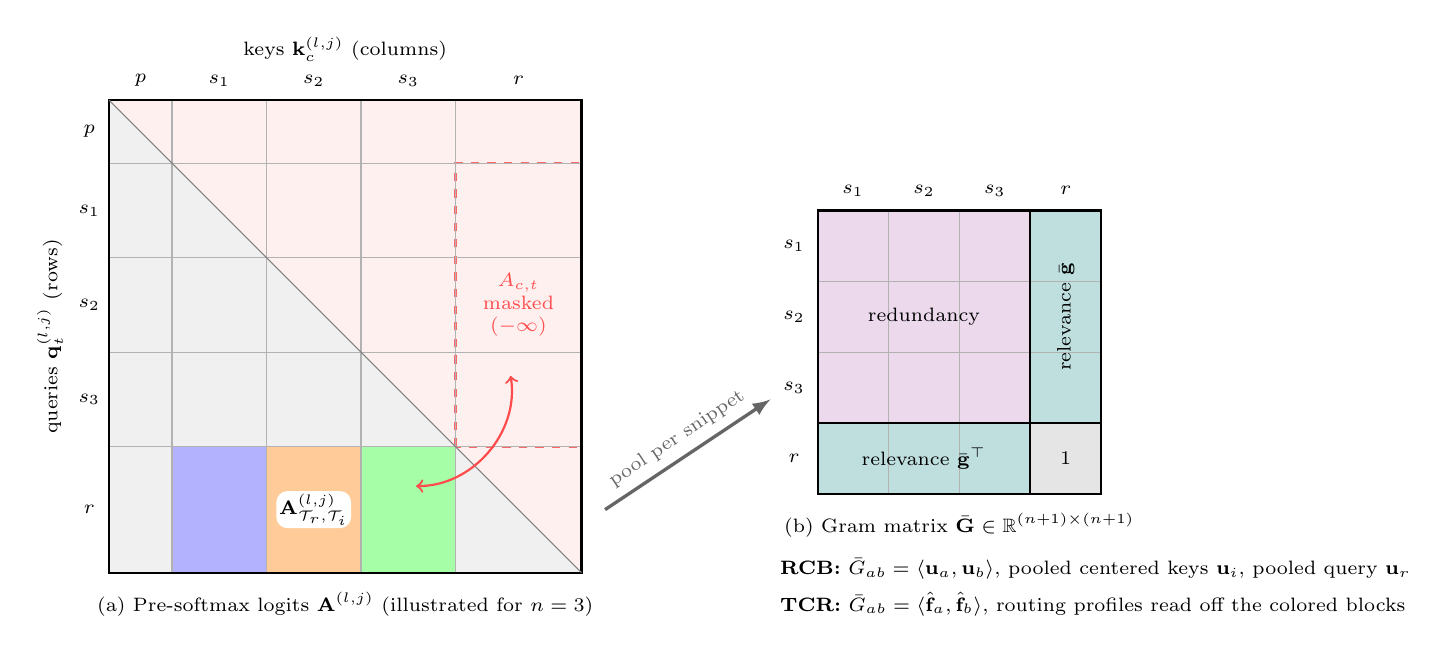
\begin{tikzpicture}[font=\scriptsize]
    % ---------------- (a) Pre-softmax logit matrix ----------------
    \fill[red!6]   (0,6) -- (6,6) -- (6,0) -- cycle;
    \fill[gray!12] (0,6) -- (0,0) -- (6,0) -- cycle;
    % causal blocks A_{T_r, T_i}
    \fill[blue!30]   (0.8,0) rectangle (2.0,1.6);
    \fill[orange!40] (2.0,0) rectangle (3.2,1.6);
    \fill[green!35]  (3.2,0) rectangle (4.4,1.6);
    % mirrored (masked) blocks A_{T_i, T_r}
    \draw[dashed, thick, red!60] (4.4,1.6) rectangle (6,5.2);
    % segment boundaries
    \foreach \x in {0.8,2.0,3.2,4.4} { \draw[gray!60] (\x,0) -- (\x,6); }
    \foreach \y in {5.2,4.0,2.8,1.6} { \draw[gray!60] (0,\y) -- (6,\y); }
    \draw[thick] (0,0) rectangle (6,6);
    \draw[gray] (0,6) -- (6,0);
    % column / row labels
    \node at (0.4,6.25) {$p$};   \node at (1.4,6.25) {$s_1$}; \node at (2.6,6.25) {$s_2$};
    \node at (3.8,6.25) {$s_3$}; \node at (5.2,6.25) {$r$};
    \node at (-0.25,5.6) {$p$};   \node at (-0.25,4.6) {$s_1$}; \node at (-0.25,3.4) {$s_2$};
    \node at (-0.25,2.2) {$s_3$}; \node at (-0.25,0.8) {$r$};
    \node at (3,6.65) {keys $\mathbf{k}^{(l,j)}_c$ (columns)};
    \node[rotate=90] at (-0.75,3) {queries $\mathbf{q}^{(l,j)}_t$ (rows)};
    \node[align=center, text=red!70] at (5.2,3.4) {$A_{c,t}$\\masked\\($-\infty$)};
    \node[fill=white, inner sep=1pt, rounded corners] at (2.6,0.8) {$\mathbf{A}^{(l,j)}_{\mathcal{T}_r,\mathcal{T}_i}$};
    \draw[<->, thick, red!70] (3.9,1.1) to[bend right=50] (5.1,2.5);
    \node at (3,-0.4) {(a) Pre-softmax logits $\mathbf{A}^{(l,j)}$ (illustrated for $n=3$)};
    % arrow
    \draw[-latex, very thick, black!60] (6.3,0.8) -- (8.4,2.2) node[midway, above, sloped] {pool per snippet};
    % ---------------- (b) Resulting Gram matrix ----------------
    \begin{scope}[shift={(9,1.0)}]
        \fill[violet!15] (0,0.9)   rectangle (2.7,3.6);
        \fill[teal!25]   (2.7,0.9) rectangle (3.6,3.6);
        \fill[teal!25]   (0,0)     rectangle (2.7,0.9);
        \fill[gray!20]   (2.7,0)   rectangle (3.6,0.9);
        \draw[step=0.9, gray!60] (0,0) grid (3.6,3.6);
        \draw[thick] (0,0) rectangle (3.6,3.6);
        \draw[thick] (2.7,0) -- (2.7,3.6);
        \draw[thick] (0,0.9) -- (3.6,0.9);
        \node at (3.15,0.45) {$1$};
        \node at (1.35,2.25) {redundancy};
        \node[rotate=90] at (3.15,2.25) {relevance $\bar{\mathbf{g}}$};
        \node at (1.35,0.45) {relevance $\bar{\mathbf{g}}^\top$};
        \node at (0.45,3.85) {$s_1$}; \node at (1.35,3.85) {$s_2$};
        \node at (2.25,3.85) {$s_3$}; \node at (3.15,3.85) {$r$};
        \node at (-0.3,3.15) {$s_1$}; \node at (-0.3,2.25) {$s_2$};
        \node at (-0.3,1.35) {$s_3$}; \node at (-0.3,0.45) {$r$};
        \node at (1.8,-0.4) {(b) Gram matrix $\bar{\mathbf{G}} \in \mathbb{R}^{(n+1)\times(n+1)}$};
    \end{scope}
    \node[anchor=west] at (8.4,0.05)  {\textbf{RCB:} $\bar{G}_{ab} = \langle \mathbf{u}_a, \mathbf{u}_b \rangle$, pooled centered keys $\mathbf{u}_i$, pooled query $\mathbf{u}_r$};
    \node[anchor=west] at (8.4,-0.4)  {\textbf{TCR:} $\bar{G}_{ab} = \langle \hat{\mathbf{f}}_a, \hat{\mathbf{f}}_b \rangle$, routing profiles read off the colored blocks};
\end{tikzpicture}%
}
\caption{Construction of the attention Gram matrices. (a)~Pre-softmax logits of one head. The colored causal blocks $\mathbf{A}^{(l,j)}_{\mathcal{T}_r, \mathcal{T}_i}$ contain the logits with which response tokens query snippet $s_i$; they are never masked. The dashed region contains the mirrored anti-causal entries, which are masked and receive no gradient; symmetrization $\frac{1}{2}(\mathbf{A} + \mathbf{A}^\top)$ pairs each colored entry with one of them (red arrow). (b)~Both constructions map each snippet and the response to one vector, which yields an $(n+1) \times (n+1)$ PSD Gram matrix. Its snippet--response entries are derived from the colored blocks: in RCB they are head-averaged centered logits of these blocks (Proposition~\ref{prop:rcb}), and in TCR they compare the routing profiles extracted from them.}
\label{fig:gram_construction}
\end{figure}

\subsubsection{Role-Aligned Causal Bilinear (RCB) Gram}
\label{subsubsec:rcb}

RCB represents each player in the role it plays in the causal logit $\langle \mathbf{q}_t, \mathbf{k}_c \rangle$: snippets as \emph{keys} and the response as a \emph{query}.

\begin{enumerate}
    \item \textbf{Anchor tokens.} Let $\bar{A}_c := \frac{1}{m |\mathcal{T}_r|} \sum_{l \in \mathcal{L}_{\text{glob}}} \sum_{j=1}^{h} \sum_{t \in \mathcal{T}_r} A^{(l,j)}_{t,c}$ be the mean causal logit received by the context token $c \in \mathcal{T}_{\text{ctx}}$. Let $\mathcal{T}_i^{\text{top}} \subseteq \mathcal{T}_i$ be the $k_0$ tokens of $s_i$ with the largest $\bar{A}_c$ (or all of $\mathcal{T}_i$ if $|\mathcal{T}_i| \le k_0$).
    \item \textbf{Centered snippet keys.} With the mean context key $\bar{\mathbf{k}}_{\text{ctx}}^{(l,j)} := \frac{1}{|\mathcal{T}_{\text{ctx}}|} \sum_{c \in \mathcal{T}_{\text{ctx}}} \mathbf{k}_c^{(l,j)}$, define
    \begin{align}
        \tilde{\mathbf{k}}_i^{(l,j)} := \operatorname{Normalize}\Big( \frac{1}{|\mathcal{T}_i^{\text{top}}|} \sum_{c \in \mathcal{T}_i^{\text{top}}} \mathbf{k}_c^{(l,j)} - \bar{\mathbf{k}}_{\text{ctx}}^{(l,j)} \Big), \qquad \mathbf{u}_i := \operatorname{Normalize}\big( \operatorname{stack}(\tilde{\mathbf{k}}_i) \big).
    \end{align}
    \item \textbf{Response query.}
    \begin{align}
        \tilde{\mathbf{q}}_r^{(l,j)} := \operatorname{Normalize}\Big( \frac{1}{|\mathcal{T}_r|} \sum_{t \in \mathcal{T}_r} \mathbf{q}_t^{(l,j)} \Big), \qquad \mathbf{u}_r := \operatorname{Normalize}\big( \operatorname{stack}(\tilde{\mathbf{q}}_r) \big).
    \end{align}
    \item \textbf{Gram matrix.} $\bar{\mathbf{G}}^{\text{RCB}} := (\langle \mathbf{u}_a, \mathbf{u}_b \rangle)_{a,b \in [n] \cup \{r\}}$ as in~\eqref{eq:attn_gram_blocks}.
\end{enumerate}

\begin{proposition}[Properties of the RCB Gram]\label{prop:rcb}
Assume that all centered snippet keys and pooled response queries are non-zero.
\begin{enumerate}
    \item[(i)] $\bar{\mathbf{G}}^{\text{RCB}}$ is symmetric PSD with unit diagonal.
    \item[(ii)] \textbf{Centering does not change attention.} For every query $\mathbf{q}$ and every vector $\bar{\mathbf{k}}$, $\operatorname{softmax}_c\big(\langle \mathbf{q}, \mathbf{k}_c - \bar{\mathbf{k}} \rangle / \sqrt{d_k}\big) = \operatorname{softmax}_c\big(\langle \mathbf{q}, \mathbf{k}_c \rangle / \sqrt{d_k}\big)$.
    \item[(iii)] \textbf{Cross-terms are averaged causal logits.} The relevance entries are head-averaged cosines,
    \begin{align}
        \langle \mathbf{u}_i, \mathbf{u}_r \rangle = \frac{1}{m} \sum_{l \in \mathcal{L}_{\text{glob}}} \sum_{j=1}^h \cos\big(\tilde{\mathbf{k}}_i^{(l,j)}, \tilde{\mathbf{q}}_r^{(l,j)}\big),
    \end{align}
    and before the per-head normalization, each summand is the centered mean logit of the causal block:
    \begin{align}\label{eq:rcb_block_logit}
        \Big\langle \frac{1}{|\mathcal{T}_r|} \sum_{t \in \mathcal{T}_r} \mathbf{q}_t^{(l,j)}, \; \frac{1}{|\mathcal{T}_i^{\text{top}}|} \sum_{c \in \mathcal{T}_i^{\text{top}}} \mathbf{k}_c^{(l,j)} - \bar{\mathbf{k}}_{\text{ctx}}^{(l,j)} \Big\rangle = \sqrt{d_k} \Big( \operatorname*{mean}_{t \in \mathcal{T}_r,\, c \in \mathcal{T}_i^{\text{top}}} A^{(l,j)}_{t,c} - \operatorname*{mean}_{t \in \mathcal{T}_r,\, c \in \mathcal{T}_{\text{ctx}}} A^{(l,j)}_{t,c} \Big).
    \end{align}
\end{enumerate}
\end{proposition}

\begin{proof}
(i) $\bar{\mathbf{G}}^{\text{RCB}}$ is the Gram matrix of $n+1$ unit vectors. (ii) Subtracting $\bar{\mathbf{k}}$ shifts every logit in the row by the same constant $\langle \mathbf{q}, \bar{\mathbf{k}} \rangle / \sqrt{d_k}$, and softmax is invariant to such shifts. (iii) $\operatorname{stack}(\tilde{\mathbf{k}}_i)$ concatenates $m$ unit vectors and therefore has norm $\sqrt{m}$, and likewise for $\operatorname{stack}(\tilde{\mathbf{q}}_r)$. Hence $\langle \mathbf{u}_i, \mathbf{u}_r \rangle = \frac{1}{m} \sum_{l,j} \langle \tilde{\mathbf{k}}_i^{(l,j)}, \tilde{\mathbf{q}}_r^{(l,j)} \rangle$. Identity~\eqref{eq:rcb_block_logit} follows from the bilinearity of the inner product and~\eqref{eq:sdpa_dot}.
\end{proof}

By (ii), centering removes a component shared by all keys that is invisible to the model's routing but would otherwise dominate the cosine similarities. By (iii), the relevance entries of RCB are, up to per-head normalization, the centered logits of exactly the causal blocks in Figure~\ref{fig:gram_construction}(a). The redundancy block compares snippets in key space: two snippets with similar keys are retrieved by the same queries and therefore act as substitutes. Note that the model never computes key--key inner products itself, so this block is a proxy for redundancy.

\subsubsection{Thresholded Causal Routing (TCR) Gram}
\label{subsubsec:tcr}

TCR represents each snippet by \emph{which heads route to it at which decoding steps}. It uses the logits of the causal blocks only. Let $\mathcal{I} := \mathcal{L}_{\text{glob}} \times [h] \times \mathcal{T}_r$ be the index set of (layer, head, response token) triples, with $D := |\mathcal{I}| = m |\mathcal{T}_r|$.

\begin{enumerate}
    \item \textbf{Background threshold.} For each $(l,j,t) \in \mathcal{I}$, let $\tau_{l,j,t} := \operatorname{Quantile}_\kappa\{A^{(l,j)}_{t,c} : c \in \mathcal{T}_{\text{ctx}}\}$ be the $\kappa$-quantile of the logits of row $t$ over the context ($\kappa = 0.9$ in our experiments, additionally capped at the median over snippets of the top-$k_0$ logit).
    \item \textbf{Snippet routing profiles.} Let $\mathcal{T}_i^{\text{top}}(l,j,t) \subseteq \mathcal{T}_i$ be the $k_0$ tokens of $s_i$ with the largest logit $A^{(l,j)}_{t,c}$. The profile $\mathbf{f}_i \in \mathbb{R}_{\ge 0}^{D}$ has entries
    \begin{align}
        f_i(l,j,t) := \frac{1}{k_0} \sum_{c \in \mathcal{T}_i^{\text{top}}(l,j,t)} \big( A^{(l,j)}_{t,c} - \tau_{l,j,t} \big)^+.
    \end{align}
    \item \textbf{Response profile.} $f_r(l,j,t) := \max_{i \in [n]} f_i(l,j,t)$, i.e., the strongest routing to any snippet at each coordinate.
    \item \textbf{Gram matrix.} With $\hat{\mathbf{f}}_a := \operatorname{Normalize}(\mathbf{f}_a)$, set $\mathbf{u}_a := \hat{\mathbf{f}}_a$ and $\bar{\mathbf{G}}^{\text{TCR}} := (\langle \hat{\mathbf{f}}_a, \hat{\mathbf{f}}_b \rangle)_{a,b \in [n] \cup \{r\}}$.
\end{enumerate}

\begin{proposition}[Properties of the TCR Gram]\label{prop:tcr}
\begin{enumerate}
    \item[(i)] $\bar{\mathbf{G}}^{\text{TCR}}$ is symmetric PSD and entrywise non-negative.
    \item[(ii)] \textbf{Inactive snippets are null players.} If $s_i$ never exceeds the threshold ($\mathbf{f}_i = \mathbf{0}$), then $\phi_i(v_{\text{logvol}}) = 0$.
    \item[(iii)] \textbf{Disjoint routing.} If the supports of $\mathbf{f}_1, \dots, \mathbf{f}_n$ are pairwise disjoint and $\mathbf{f}_r \neq \mathbf{0}$, then $\mathbf{f}_r = \sum_i \mathbf{f}_i$, and the squared relevance entries $\langle \hat{\mathbf{f}}_i, \hat{\mathbf{f}}_r \rangle^2 = \|\mathbf{f}_i\|_2^2 / \|\mathbf{f}_r\|_2^2$ sum to one. They are the shares of the routing energy received by each snippet.
\end{enumerate}
\end{proposition}

\begin{proof}
(i) Gram matrix of non-negative vectors. (ii) $\hat{\mathbf{f}}_i = \mathbf{0}$ does not change the span of any coalition, so $d_{\perp}(\mathbf{r}, \mathcal{U}_{\{S' \cup \{i\}\}}) = d_{\perp}(\mathbf{r}, \mathcal{U}_{\{S'\}})$ and $\Delta v_{\text{logvol}}(S', i) = 0$ for all $S'$; apply the Null player axiom. (iii) With disjoint supports, the coordinate-wise maximum equals the sum, and $\langle \mathbf{f}_i, \mathbf{f}_r \rangle = \|\mathbf{f}_i\|_2^2$. Orthogonality gives $\|\mathbf{f}_r\|_2^2 = \sum_i \|\mathbf{f}_i\|_2^2$.
\end{proof}

Snippets that activate the same heads at the same decoding steps have a large inner product and therefore share their Shapley credit, while snippets routed through different heads or steps receive complementary credit, as in multi-hop reasoning. In the setting of (iii), the response lies in the span of all snippets, so $v_{\text{logvol}}([n]) = \infty$, and the regularized value function of~\eqref{eq:marginal_sherman} must be used.

\paragraph{Comparison.}
RCB uses pooled query and key \emph{vectors}. Its cost is $\mathcal{O}(N d_{\text{attn}})$, and it has a single hyperparameter $k_0$. TCR uses only the logits of the causal blocks, which can be computed from the cached queries of $\mathcal{T}_r$ and keys of $\mathcal{T}_{\text{ctx}}$ without materializing $\mathbf{A}^{(l,j)}$, at cost $\mathcal{O}(m |\mathcal{T}_r| |\mathcal{T}_{\text{ctx}}| d_k)$. It has two hyperparameters, $k_0$ and $\kappa$. RCB measures \emph{alignment} of representations, whereas TCR measures \emph{actual routing above background}.

\subsection{From the Attention Gram to Attributions}
\label{subsec:gatt_pipeline}

Given either construction, attributions are computed as follows.
\begin{enumerate}
    \item \textbf{Forward pass.} Run the model once on $(p, S, r)$ (this can be the generation pass itself) and cache $\mathbf{q}_t^{(l,j)}$, $\mathbf{k}_c^{(l,j)}$ for $t \in \mathcal{T}_r$, $c \in \mathcal{T}_{\text{ctx}}$ and $l \in \mathcal{L}_{\text{glob}}$.
    \item \textbf{Gram matrix.} Build $\bar{\mathbf{G}} \in \mathbb{R}^{(n+1) \times (n+1)}$ by RCB or TCR.
    \item \textbf{Value function.} Substitute $\mathbf{G}_{\{S'\}} := \bar{\mathbf{G}}_{S',S'}$ and $\mathbf{g}_{\{S'\}} := \bar{\mathbf{g}}_{S'}$ into the value functions of Section~\ref{subsec:geometric_values}. All three depend on these blocks only. $v_{\text{vol}}$ uses determinants. $v_{\text{logvol}}(S') = -\frac{1}{2}\log\big(1 - \mathbf{g}_{\{S'\}}^\top \mathbf{G}_{\{S'\}}^{\dagger} \mathbf{g}_{\{S'\}}\big)$ follows from Lemma~\ref{lem:vol_factorization}. $v_{\text{ent}}$ uses the eigenvalues of $\bar{\mathbf{G}}_{S' \cup \{r\}, S' \cup \{r\}}$. Once $\bar{\mathbf{G}}$ is built, the $d_{\text{attn}}$-dimensional vectors are no longer needed. To keep $v_{\text{logvol}}$ finite, replace $\mathbf{G}_{\{S'\}}$ by $\mathbf{G}_{\{S'\}} + \lambda \mathbf{I}$.
    \item \textbf{Shapley values.} For small $n$, enumerate all $2^n$ coalitions, with each evaluation costing $\mathcal{O}(|S'|^3)$, or $\mathcal{O}(|S'|^2)$ with incremental Cholesky updates. Otherwise, average marginal gains over $K$ random permutations, which is unbiased by Lemma~\ref{lemma:unbiased_estimator}.
    \item \textbf{Link and global weight.} Map $\boldsymbol{\phi}$ to the simplex with a link function (Section~\ref{subsec:link_functions}), applied once to the averaged estimate, and scale by $w$. Computing $w$ requires $\log P(r \mid p, S)$, available from step~1, and $\log P(r \mid p)$, which requires \emph{one additional} prompt-only forward pass.
\end{enumerate}
Thus, GATT requires two forward passes in total, one of which can be shared with generation, independently of $n$. By contrast, likelihood-based Shapley estimation requires $Kn + 1$ passes (Section~\ref{sec:llh_shapley}).

\subsection{Background Floor and Contrast Calibration}
\label{subsec:contrast_calibration}

Empirically, distractor snippets receive positive Shapley values of similar magnitude under both constructions. All context tokens share components driven by the common prompt, the positional encoding, and syntax, and part of the attention mass is absorbed by sink tokens irrespective of content~\cite{xiao2024efficient}. As a stylized model, suppose that $v = v_0 + b\,|S'|$, i.e., every snippet contributes a fixed amount $b > 0$ independently of the coalition. Since $\boldsymbol{\phi}$ is linear and the additive game $b\,|S'|$ has Shapley vector $b\mathbf{1}$, we get $\boldsymbol{\phi}(v) = \boldsymbol{\phi}(v_0) + b\mathbf{1}$. Under the linear or rectified link, each distractor then receives a share of order $b / v([n])$, which inflates distractor mass without changing the ranking. We resolve this issue by using Floor-shifted power link. This is the power link of Section~\ref{subsec:link_functions} applied to $\boldsymbol{\phi} - \phi_{\min}\mathbf{1}$. For $\gamma = 1$ it only removes the floor, and $\gamma > 1$ additionally sharpens the distribution ($\gamma = 2$ in our experiments).

\begin{proposition}[Properties of the floor-shifted power link]\label{prop:rank_invariance}
For every $\gamma > 0$:
\begin{enumerate}
    \item[(i)] $g^{\text{fl},\gamma}(\boldsymbol{\phi}) \in \Delta^{n-1}$.
    \item[(ii)] \textbf{Order preservation.} $\phi_i > \phi_k \Leftrightarrow g^{\text{fl},\gamma}_i(\boldsymbol{\phi}) > g^{\text{fl},\gamma}_k(\boldsymbol{\phi})$. Hence all within-example ordinal metrics (AUROC, Spearman's $\rho$, Kendall's $\tau$, Precision@$k$, top-1 agreement) coincide with those of $\boldsymbol{\phi}$.
    \item[(iii)] \textbf{Floor removal.} Every snippet attaining $\phi_{\min}$ receives zero contribution.
    \item[(iv)] \textbf{Affine invariance.} $g^{\text{fl},\gamma}(c\boldsymbol{\phi} + b\mathbf{1}) = g^{\text{fl},\gamma}(\boldsymbol{\phi})$ for all $c > 0$ and $b \in \mathbb{R}$. In particular, (P3) holds, and the floor $b\mathbf{1}$ of the stylized model above is removed exactly.
    \item[(v)] It violates Null player (P2) and Faithfulness (P4).
\end{enumerate}
\end{proposition}

\begin{proof}
(i) If not all $\phi_j$ are equal, the numerators are non-negative and their sum is positive; otherwise, the output is uniform. (ii) $x \mapsto (x - \phi_{\min})^\gamma$ is strictly increasing on $[\phi_{\min}, \infty)$, and the normalization is a common positive factor. (iii) $(\phi_{\min} - \phi_{\min})^\gamma = 0$. (iv) Both $\phi_i - \phi_{\min}$ and the normalization are invariant to $b$, and the factor $c^\gamma$ cancels. (v) For $\boldsymbol{\phi} = (-1, 0, 2)$, the null player $i = 2$ receives $1/(1 + 3^\gamma) > 0$. For $\boldsymbol{\phi} = (2, 1)$, the output $(1, 0)$ differs from $\boldsymbol{\phi}/\mathbf{1}^\top\boldsymbol{\phi} = (2/3, 1/3)$.
\end{proof}

By (iv), the floor-shifted link is the natural choice when Shapley values contain a common offset. However, (iii) and (v) come at a price: the snippet with the lowest Shapley value always receives zero credit, even if every snippet supports the response. The link is therefore appropriate when the retrieved context is known to contain at least one distractor, and results should also be reported with the rectified link. Since it is non-linear, it must be applied to the averaged Monte Carlo estimate rather than to individual permutations.


%%%%%%%%%%%%%%%%%%%%%%%%%%%%%%%%%%%%%%%%%%%%%%%%%%%%%%%%%%%%%%%%%%%%%%%%%%%%%%%%%%%%%%%%%%%%%%%%%%%%%%%%%%%%
%%%%%%%%%%%%%%%%%%%%%%%%%%%%%%%%%%%%%%%%%%%%%%%%%%%%%%%%%%%%%%%%%%%%%%%%%%%%%%%%%%%%%%%%%%%%%%%%%%%%%%%%%%%%


\section{Set-Valued Embedding Games}
\label{sec:set_embeddings}

The value functions of Section~\ref{subsec:geometric_values} represent every player by a \emph{single} unit vector: the snippet $s_i$ by $\mathbf{m}_i = f(s_i)$ and the response by $\mathbf{r} = f(r)$. A snippet, however, is a sequence of tokens, and a transformer represents it by one vector per token in every layer and head. Pooling these vectors into one vector discards information: two snippets can have nearly identical mean embeddings and still support entirely different facts, and a response that combines a date from one snippet with a name from another is poorly described by the mean of its token embeddings. In this section, we extend the three value functions to players that are represented by \emph{sets} of vectors, i.e., by subspaces, and we then apply the extension to the value vectors of the transformer that generated the response. The players of the cooperative game remain the $n$ snippets; only their geometric representation changes. All axiomatic guarantees of Section~\ref{sec:coop_game} therefore continue to hold.

\subsection{Players as Sets of Vectors}
\label{subsec:set_notation}

Each snippet $s_i$ is represented by a matrix $\mathbf{M}_i \in \mathbb{R}^{d \times N_i}$ whose $N_i$ columns are vectors associated with $s_i$, e.g., the contextual embeddings of its tokens. Likewise, the response is represented by $\mathbf{R} = [\mathbf{r}_1, \dots, \mathbf{r}_{N_r}] \in \mathbb{R}^{d \times N_r}$, together with non-negative weights $\omega_1, \dots, \omega_{N_r}$ that sum to one (uniform unless stated otherwise). For a coalition $S' \subseteq [n]$, we concatenate the matrices of its members,
\begin{align}
    \mathbf{M}_{\{S'\}} := \big[\mathbf{M}_i\big]_{i \in S'} \in \mathbb{R}^{d \times N_{S'}}, \qquad N_{S'} := \sum_{i \in S'} N_i,
\end{align}
and denote by $\mathcal{U}_i := \operatorname{span}(\mathbf{M}_i)$, $\mathcal{U}_{\{S'\}} := \operatorname{span}(\mathbf{M}_{\{S'\}}) = \sum_{i \in S'} \mathcal{U}_i$ and $\mathcal{U}_R := \operatorname{span}(\mathbf{R})$ the corresponding subspaces, with $\mathcal{U}_{\emptyset} := \{\mathbf{0}\}$. The orthogonal projection onto $\mathcal{U}_{\{S'\}}$ is $\mathbf{P}_{\{S'\}} := \mathbf{M}_{\{S'\}} \mathbf{M}_{\{S'\}}^{\dagger}$, exactly as in Section~\ref{subsec:geometric_values}. The single-vector setting is the special case $N_i = N_r = 1$.

\paragraph{Block Gram matrix.}
All quantities below depend on the vectors only through the block Gram matrix
\begin{align}\label{eq:set_gram}
    \mathbf{G}^{+}_{\{S'\}} := \big[\mathbf{M}_{\{S'\}}, \mathbf{R}\big]^\top \big[\mathbf{M}_{\{S'\}}, \mathbf{R}\big] =
    \begin{bmatrix}
        \mathbf{G}_{\{S'\}} & \mathbf{C}_{\{S'\}} \\
        \mathbf{C}_{\{S'\}}^\top & \mathbf{G}_{R}
    \end{bmatrix},
\end{align}
with $\mathbf{G}_{\{S'\}} = \mathbf{M}_{\{S'\}}^\top \mathbf{M}_{\{S'\}}$, $\mathbf{C}_{\{S'\}} = \mathbf{M}_{\{S'\}}^\top \mathbf{R}$ and $\mathbf{G}_{R} = \mathbf{R}^\top \mathbf{R}$.
It generalizes $\mathbf{G}^{+}_{\{S'\}}$ of Section~\ref{subsec:geometric_values}: the scalar entries $\langle \mathbf{m}_i, \mathbf{m}_j \rangle$, $\langle \mathbf{m}_i, \mathbf{r} \rangle$ and $1$ become the blocks $\mathbf{M}_i^\top \mathbf{M}_j$, $\mathbf{M}_i^\top \mathbf{R}$ and $\mathbf{G}_R$. The diagonal blocks $\mathbf{M}_i^\top \mathbf{M}_i$ describe the internal geometry of a snippet, the off-diagonal blocks $\mathbf{M}_i^\top \mathbf{M}_j$ the redundancy between snippets, and $\mathbf{C}_{\{S'\}}$ the relevance of the snippets to the response tokens. Exactly as for GATT (Section~\ref{subsec:gatt_pipeline}), the vectors are no longer needed once the Gram matrix of all $N_{[n]} + N_r$ vectors has been computed.

\paragraph{Principal angles.}
The natural generalization of the angle between $\mathbf{r}$ and $\mathcal{U}_{\{S'\}}$ is the sequence of principal angles between subspaces~\cite{bjorck1973numerical}. Let $\mathbf{Q}_R \in \mathbb{R}^{d \times k_r}$ be an orthonormal basis of $\mathcal{U}_R$ (or of a truncation of it, see Section~\ref{subsec:set_regularization}). The principal angles $0 \le \theta_1(S') \le \dots \le \theta_{k_r}(S') \le \pi/2$ between $\mathcal{U}_R$ and $\mathcal{U}_{\{S'\}}$ are defined by
\begin{align}\label{eq:principal_angles}
    \cos^2 \theta_k(S') := \lambda_k\big(\mathbf{Q}_R^\top \mathbf{P}_{\{S'\}} \mathbf{Q}_R\big), \qquad k \in [k_r],
\end{align}
where $\lambda_1 \ge \dots \ge \lambda_{k_r}$ denote the eigenvalues in decreasing order. For $k_r = 1$ and $\mathbf{Q}_R = \mathbf{r}$, $\sin \theta_1(S') = d_{\perp}(\mathbf{r}, \mathcal{U}_{\{S'\}})$.

\paragraph{Orthonormal player bases.}
Unit normalization in the single-vector setting ensures that a player's value does not depend on the norm of its embedding. The set-valued analogue is to represent each player by an orthonormal basis $\mathbf{Q}_i \in \mathbb{R}^{d \times k_i}$ of $\mathcal{U}_i$ (or of its dominant $k_i$-dimensional part). Then the diagonal blocks of $\mathbf{G}_{\{S'\}}$ are identity matrices, $\operatorname{Tr}(\mathbf{G}^{+}_{\{S'\}}) = \sum_{i \in S'} k_i + k_r$, and the off-diagonal blocks $\mathbf{Q}_i^\top \mathbf{Q}_j$ have the cosines of the principal angles between $\mathcal{U}_i$ and $\mathcal{U}_j$ as singular values. Redundancy \emph{within} a snippet (many tokens that encode the same content) then no longer affects the value, while redundancy \emph{between} snippets does. The projection-based value functions $v_{\text{proj}}$ and $v_{\text{logvol}}$ below depend only on the subspaces and are therefore unaffected by this choice; $v_{\text{vol}}$ and $v_{\text{ent}}$ require it.

\subsection{Set-Valued Value Functions}
\label{subsec:set_values}

The volume factorization of Lemma~\ref{lem:vol_factorization} generalizes verbatim, with the scalar residual $d_{\perp}^2$ replaced by the Gram matrix of the residual response vectors.

\begin{lemma}[Block Volume Factorization]\label{lem:block_vol_factorization}
For every coalition $S' \subseteq [n]$ such that $\mathbf{M}_{\{S'\}}$ has full column rank,
\begin{align}
    \det \mathbf{G}^{+}_{\{S'\}} = \det \mathbf{G}_{\{S'\}} \cdot \det \boldsymbol{\Sigma}_{R \mid S'}, \qquad
    \boldsymbol{\Sigma}_{R \mid S'} := \mathbf{G}_R - \mathbf{C}_{\{S'\}}^\top \mathbf{G}_{\{S'\}}^{-1} \mathbf{C}_{\{S'\}} = \mathbf{R}^\top (\mathbf{I}_d - \mathbf{P}_{\{S'\}}) \mathbf{R}.
\end{align}
If, moreover, $\mathbf{R} = \mathbf{Q}_R$ has orthonormal columns, then $\det \boldsymbol{\Sigma}_{R \mid S'} = \prod_{k=1}^{k_r} \sin^2 \theta_k(S')$.
\end{lemma}

\begin{proof}
The first identity is Schur's determinant formula for the block matrix~\eqref{eq:set_gram}; the second expression for $\boldsymbol{\Sigma}_{R \mid S'}$ follows from $\mathbf{P}_{\{S'\}} = \mathbf{M}_{\{S'\}} \mathbf{G}_{\{S'\}}^{-1} \mathbf{M}_{\{S'\}}^\top$. If $\mathbf{R} = \mathbf{Q}_R$, then $\boldsymbol{\Sigma}_{R \mid S'} = \mathbf{I}_{k_r} - \mathbf{Q}_R^\top \mathbf{P}_{\{S'\}} \mathbf{Q}_R$, whose eigenvalues are $1 - \cos^2 \theta_k(S') = \sin^2 \theta_k(S')$ by~\eqref{eq:principal_angles}.
\end{proof}

\paragraph{Projected Response Energy ($v_{\text{proj}}$).}
The most direct way to ask how much of the response is explained by a coalition is to project every response vector onto the coalition subspace and to measure the fraction of the response energy that is captured:
\begin{align}\label{eq:v_proj}
    v_{\text{proj}}(S') := \frac{\sum_{t=1}^{N_r} \omega_t \, \|\mathbf{P}_{\{S'\}} \mathbf{r}_t\|_2^2}{\sum_{t=1}^{N_r} \omega_t \, \|\mathbf{r}_t\|_2^2} = \frac{\operatorname{Tr}\big(\boldsymbol{\Omega}^{1/2} \mathbf{C}_{\{S'\}}^\top \mathbf{G}_{\{S'\}}^{\dagger} \mathbf{C}_{\{S'\}} \boldsymbol{\Omega}^{1/2}\big)}{\operatorname{Tr}\big(\boldsymbol{\Omega}^{1/2} \mathbf{G}_R \boldsymbol{\Omega}^{1/2}\big)} \in [0, 1],
\end{align}
with $\boldsymbol{\Omega} := \operatorname{diag}(\omega_1, \dots, \omega_{N_r})$ and $v_{\text{proj}}(\emptyset) = 0$. In the single-vector setting, $v_{\text{proj}}(S') = \mathbf{r}^\top \mathbf{P}_{\{S'\}} \mathbf{r} = 1 - d_{\perp}^2(\mathbf{r}, \mathcal{U}_{\{S'\}})$, a monotone transformation of $v_{\text{logvol}}$; we did not list it separately in Section~\ref{subsec:geometric_values} for this reason. For sets, the two differ: $v_{\text{proj}}$ averages the explained energy over the response, whereas $v_{\text{logvol}}$ below rewards explaining \emph{every} response direction. If the response is represented by an orthonormal basis with uniform weights, $v_{\text{proj}}(S') = \frac{1}{k_r} \sum_{k} \cos^2 \theta_k(S')$.

Since $v_{\text{proj}}$ is a weighted average of the per-token games $v_t(S') := \|\mathbf{P}_{\{S'\}} \mathbf{r}_t\|_2^2 / \|\mathbf{r}_t\|_2^2$, the Linearity axiom yields a token-level decomposition of every snippet's credit,
\begin{align}\label{eq:v_proj_token_decomposition}
    \phi_i(v_{\text{proj}}) = \sum_{t=1}^{N_r} \tilde{\omega}_t \, \phi_i(v_t), \qquad \tilde{\omega}_t := \frac{\omega_t \|\mathbf{r}_t\|_2^2}{\sum_{t'} \omega_{t'} \|\mathbf{r}_{t'}\|_2^2},
\end{align}
which states which response tokens are explained by which snippets.

\paragraph{Principal-Angle Log-Volume ($v_{\text{logvol}}$).}
Following~\eqref{eq:v_logvol}, we define the log-volume value function as the negative log-volume of the residual of the (orthonormalized) response:
\begin{align}\label{eq:set_v_logvol}
    v_{\text{logvol}}(S') := -\frac{1}{2} \log \det \big(\mathbf{I}_{k_r} - \mathbf{Q}_R^\top \mathbf{P}_{\{S'\}} \mathbf{Q}_R\big) = -\sum_{k=1}^{k_r} \log \sin \theta_k(S'),
\end{align}
with $v_{\text{logvol}}(\emptyset) = 0$. By Lemma~\ref{lem:block_vol_factorization}, this is again the difference of the log-volumes with and without the response, $\log \operatorname{Vol}(\mathbf{M}_{\{S'\}}) - \log \operatorname{Vol}([\mathbf{M}_{\{S'\}}, \mathbf{Q}_R])$. The Gaussian channel of Theorem~\ref{thm:gaussian_equivalence} extends to a vector-valued response: if $\mathbf{z} \sim \mathcal{N}(\mathbf{0}, \mathbf{I}_d)$, $X_{S'} := \mathbf{M}_{\{S'\}}^\top \mathbf{z}$ and $Y := \mathbf{Q}_R^\top \mathbf{z}$, then $\operatorname{Cov}(Y \mid X_{S'}) = \mathbf{I}_{k_r} - \mathbf{Q}_R^\top \mathbf{P}_{\{S'\}} \mathbf{Q}_R$ and therefore $v_{\text{logvol}}(S') = I(Y; X_{S'})$, the Shannon mutual information between the response and the coalition. Every principal angle contributes additively: a coalition that explains only half of the response directions perfectly still leaves $\sin \theta_k = 1$ for the remaining directions, which do not contribute.

\paragraph{Volume Difference ($v_{\text{vol}}$).}
With orthonormal player bases $\mathbf{Q}_i$ and response basis $\mathbf{Q}_R$, the analogue of~\eqref{eq:v_vol} is
\begin{align}\label{eq:set_v_vol}
    v_{\text{vol}}(S') := \operatorname{Vol}(\mathbf{Q}_{\{S'\}}) - \operatorname{Vol}([\mathbf{Q}_{\{S'\}}, \mathbf{Q}_R]) = \underbrace{\operatorname{Vol}(\mathbf{Q}_{\{S'\}})}_{\text{inter-snippet diversity}} \cdot \Big(1 - \prod_{k=1}^{k_r} \sin \theta_k(S')\Big) \in [0, 1],
\end{align}
where $\mathbf{Q}_{\{S'\}} := [\mathbf{Q}_i]_{i \in S'}$ and the factorization follows from Lemma~\ref{lem:block_vol_factorization}. Because the diagonal blocks of $\mathbf{Q}_{\{S'\}}^\top \mathbf{Q}_{\{S'\}}$ are identity matrices, the base volume equals $1$ if the snippet subspaces are mutually orthogonal and shrinks with the cosines of the principal angles between them (for two snippets, $\operatorname{Vol}^2([\mathbf{Q}_i, \mathbf{Q}_j]) = \prod_k \sin^2 \theta_k(\mathcal{U}_i, \mathcal{U}_j)$ by Lemma~\ref{lem:block_vol_factorization}); it therefore penalizes only redundancy \emph{between} snippets. Without orthonormalization, the base volume of a few hundred contextual token embeddings is numerically zero, and $v_{\text{vol}}$ degenerates.

\paragraph{Spectral Entropy ($v_{\text{ent}}$).}
With orthonormal bases, the density matrix is $\boldsymbol{\rho} := \mathbf{G}^{+}_{\{S'\}} / (\sum_{i \in S'} k_i + k_r)$, and the decoupled reference $\bar{\mathbf{G}}^{+}_{\{S'\}}$ of~\eqref{eq:v_ent} sets the off-diagonal block $\mathbf{C}_{\{S'\}}$ to zero:
\begin{align}\label{eq:set_v_ent}
    v_{\text{ent}}(S') := \mathcal{H}\big(\bar{\mathbf{G}}^{+}_{\{S'\}}\big) - \mathcal{H}\big(\mathbf{G}^{+}_{\{S'\}}\big), \qquad
    \bar{\mathbf{G}}^{+}_{\{S'\}} := \begin{bmatrix} \mathbf{G}_{\{S'\}} & \mathbf{0} \\ \mathbf{0} & \mathbf{I}_{k_r} \end{bmatrix}.
\end{align}
The reference is the \emph{pinching} of $\mathbf{G}^{+}_{\{S'\}}$ onto its context and response blocks, which is what keeps $v_{\text{ent}}$ bounded by $\log 2$ independently of the number of vectors (Proposition~\ref{prop:set_values}(iv)).

\begin{proposition}[Properties of the set-valued value functions]\label{prop:set_values}
\begin{enumerate}
    \item[(i)] \textbf{Reduction.} For $N_i = N_r = 1$ and unit vectors, \eqref{eq:set_v_logvol}, \eqref{eq:set_v_vol} and~\eqref{eq:set_v_ent} coincide with~\eqref{eq:v_logvol}, \eqref{eq:v_vol} and~\eqref{eq:v_ent}, and $v_{\text{proj}} = 1 - d_{\perp}^2$.
    \item[(ii)] \textbf{Basis invariance.} $v_{\text{proj}}$ and $v_{\text{logvol}}$ depend on the snippets only through the subspaces $\mathcal{U}_i$; in particular, they are invariant to the order of the tokens and to any invertible reparametrization $\mathbf{M}_i \mapsto \mathbf{M}_i \mathbf{T}_i$.
    \item[(iii)] \textbf{Monotonicity and non-negative Shapley values.} $v_{\text{proj}}$ and $v_{\text{logvol}}$ are monotone with $v(\emptyset) = 0$. Hence $\phi_i(v) \ge 0$ for all $i$, and $\sum_i \phi_i(v_{\text{proj}}) = v_{\text{proj}}([n]) \le 1$.
    \item[(iv)] \textbf{Bounded entropy.} $0 \le v_{\text{ent}}(S') \le \log 2$ for every coalition and every number of vectors per player.
    \item[(v)] \textbf{Sets dominate pooling.} Let $\bar{\mathbf{m}}_i \in \mathcal{U}_i$ be any pooled snippet vector (e.g., a weighted mean of the columns of $\mathbf{M}_i$), and let $v^{\text{pool}}$ denote the value function computed from $\{\bar{\mathbf{m}}_i\}$ with the same response representation. Then $v^{\text{pool}}_{\text{proj}}(S') \le v_{\text{proj}}(S')$ and $v^{\text{pool}}_{\text{logvol}}(S') \le v_{\text{logvol}}(S')$ for all $S'$.
    \item[(vi)] \textbf{Orthogonal snippets decouple.} If $\mathcal{U}_i \perp \mathcal{U}_j$ for all $i \neq j$, then $v_{\text{proj}}$ is additive, and $\phi_i(v_{\text{proj}}) = v_{\text{proj}}(\{i\})$ in closed form.
\end{enumerate}
\end{proposition}

\begin{proof}
(i) Direct substitution, using Lemma~\ref{lem:vol_factorization}. (ii) $\mathbf{P}_{\{S'\}}$ depends only on $\mathcal{U}_{\{S'\}} = \sum_{i \in S'} \mathcal{U}_i$. (iii) $S' \subseteq T'$ implies $\mathcal{U}_{\{S'\}} \subseteq \mathcal{U}_{\{T'\}}$ and hence $\mathbf{P}_{\{S'\}} \preceq \mathbf{P}_{\{T'\}}$ in the Loewner order. Thus every $\|\mathbf{P}_{\{S'\}} \mathbf{r}_t\|_2^2$ is non-decreasing, and $\mathbf{I} - \mathbf{Q}_R^\top \mathbf{P}_{\{S'\}} \mathbf{Q}_R$ is non-increasing, so its log-determinant is non-increasing. Monotonicity makes all marginal gains, and hence all Shapley values, non-negative; the sum follows from Efficiency. (iv) Let $\boldsymbol{\sigma} := \bar{\mathbf{G}}^{+}_{\{S'\}} / \operatorname{Tr}(\mathbf{G}^{+}_{\{S'\}})$, which has the same trace as $\boldsymbol{\rho}$. With the Hermitian unitary $\mathbf{U} := \operatorname{diag}(\mathbf{I}, -\mathbf{I}_{k_r})$, $\boldsymbol{\sigma} = \frac{1}{2}(\boldsymbol{\rho} + \mathbf{U}\boldsymbol{\rho}\mathbf{U})$. Since $\log \boldsymbol{\sigma}$ is block diagonal and $\boldsymbol{\rho}$, $\boldsymbol{\sigma}$ share their diagonal blocks, $\operatorname{Tr}(\boldsymbol{\rho} \log \boldsymbol{\sigma}) = \operatorname{Tr}(\boldsymbol{\sigma} \log \boldsymbol{\sigma})$ and hence $v_{\text{ent}}(S') = D(\boldsymbol{\rho} \,\|\, \boldsymbol{\sigma}) \ge 0$, as in Proposition~\ref{prop:v_ent}. Moreover, $2\boldsymbol{\sigma} - \boldsymbol{\rho} = \mathbf{U}\boldsymbol{\rho}\mathbf{U} \succeq \mathbf{0}$, i.e., $\boldsymbol{\rho} \preceq 2\boldsymbol{\sigma}$, and the operator monotonicity of the logarithm gives $\log \boldsymbol{\rho} \preceq \log 2 \cdot \mathbf{I} + \log \boldsymbol{\sigma}$ on the support of $\boldsymbol{\rho}$. Taking the trace against $\boldsymbol{\rho} \succeq \mathbf{0}$ yields $D(\boldsymbol{\rho} \,\|\, \boldsymbol{\sigma}) \le \log 2$. (v) $\operatorname{span}\{\bar{\mathbf{m}}_i\}_{i \in S'} \subseteq \mathcal{U}_{\{S'\}}$, so the pooled projection is dominated in the Loewner order; argue as in (iii). (vi) Orthogonality gives $\mathbf{P}_{\{S'\}} = \sum_{i \in S'} \mathbf{P}_i$, so $v_{\text{proj}}(S') = \sum_{i \in S'} v_{\text{proj}}(\{i\})$, and the Shapley value of an additive game is its singleton value.
\end{proof}

By (v), pooling never explains more of the response than the token sets it was computed from. The difference is largest exactly in the multi-hop setting that motivates attribution: if the response contains one direction from $s_1$ and an orthogonal direction from $s_2$, the pooled vectors only capture the components of these directions that survive averaging, while the token subspaces contain both. By (vi), set-valued Shapley values reduce to a closed-form per-snippet projection when snippets are mutually orthogonal, and they differ from it precisely by how they split credit among overlapping (redundant) snippet subspaces.

\begin{table}[t]
\centering
\small
\renewcommand{\arraystretch}{1.2}
\begin{tabular}{lcccc}
\toprule
\textbf{Value function} & \textbf{Codomain} & \textbf{Monotone} & \textbf{Orthonormal bases} & \textbf{Single-vector case} \\
\midrule
$v_{\text{proj}}$ \eqref{eq:v_proj} & $[0, 1]$ & \checkmark & $\times$ & $1 - d_{\perp}^2$ \\
$v_{\text{logvol}}$ \eqref{eq:set_v_logvol} & $[0, \infty)$ & \checkmark & response only & \eqref{eq:v_logvol} \\
$v_{\text{vol}}$ \eqref{eq:set_v_vol} & $[0, 1]$ & $\times$ & \checkmark & \eqref{eq:v_vol} \\
$v_{\text{ent}}$ \eqref{eq:set_v_ent} & $[0, \log 2]$ & $\times$ & \checkmark & \eqref{eq:v_ent} \\
\bottomrule
\end{tabular}
\caption{Set-valued embedding value functions (cf.\ Table~\ref{tab:geom_value_comparison}).}
\label{tab:set_value_comparison}
\end{table}

\subsection{Regularization and Effective Rank}
\label{subsec:set_regularization}

Sets of vectors introduce a degeneracy that does not occur for single vectors. If $N_{\{S'\}} \ge d$, the columns of $\mathbf{M}_{\{S'\}}$ generically span all of $\mathbb{R}^d$; then $\mathbf{P}_{\{S'\}} = \mathbf{I}_d$, every response is fully explained, $v_{\text{logvol}}(S') = \infty$, and the game no longer discriminates between snippets. Even for $N_{\{S'\}} < d$, a long snippet spans many directions that carry little information. We use two remedies, which can be combined.

\paragraph{Ridge (soft) projection.}
Replacing the projection by the ridge operator $\mathbf{P}^{(\lambda)}_{\{S'\}} := \mathbf{M}_{\{S'\}} (\mathbf{G}_{\{S'\}} + \lambda \mathbf{I})^{-1} \mathbf{M}_{\{S'\}}^\top$, $\lambda > 0$, extends the regularization of Section~\ref{subsec:geometric_values} to sets. By the push-through identity, $\mathbf{I}_d - \mathbf{P}^{(\lambda)}_{\{S'\}} = \lambda (\lambda \mathbf{I}_d + \mathbf{M}_{\{S'\}} \mathbf{M}_{\{S'\}}^\top)^{-1}$, so
\begin{align}\label{eq:set_logvol_ridge}
    v^{(\lambda)}_{\text{logvol}}(S') := -\frac{1}{2} \log \det \Big( \lambda \, \mathbf{Q}_R^\top \big(\lambda \mathbf{I}_d + \mathbf{M}_{\{S'\}} \mathbf{M}_{\{S'\}}^\top\big)^{-1} \mathbf{Q}_R \Big) = I\big(Y; X_{S'} + \boldsymbol{\varepsilon}\big), \qquad \boldsymbol{\varepsilon} \sim \mathcal{N}(\mathbf{0}, \lambda \mathbf{I}),
\end{align}
i.e., the regularized value is the mutual information between the response and a \emph{noisy} observation of the coalition, and it is finite for every coalition. Directions of $\mathcal{U}_{\{S'\}}$ along which the snippet tokens carry energy well below $\lambda$ contribute little; the number of effectively used directions is $d_{\text{eff}}(\lambda) := \operatorname{Tr}\big(\mathbf{G}_{\{S'\}} (\mathbf{G}_{\{S'\}} + \lambda \mathbf{I})^{-1}\big)$. Since $\mathbf{A} \mapsto \mathbf{A}(\mathbf{A} + \lambda \mathbf{I})^{-1}$ is operator monotone and $\mathbf{M}_{\{S'\}} \mathbf{M}_{\{S'\}}^\top$ grows in the Loewner order with $S'$, both $v^{(\lambda)}_{\text{proj}}$ (defined by~\eqref{eq:v_proj} with $\mathbf{P}^{(\lambda)}$) and $v^{(\lambda)}_{\text{logvol}}$ remain monotone, so Proposition~\ref{prop:set_values}(iii) continues to hold. Both are computed from the block Gram matrix~\eqref{eq:set_gram} alone.

\paragraph{Rank truncation.}
Alternatively, each player is replaced by the top-$k_i$ left singular vectors $\mathbf{Q}_i$ of $\mathbf{M}_i$, with $k_i$ chosen as the smallest rank that retains a fraction $\eta$ of the energy $\|\mathbf{M}_i\|_F^2$ (and likewise $\mathbf{Q}_R$ for the response). This yields the orthonormal player bases required by $v_{\text{vol}}$ and $v_{\text{ent}}$, makes every coalition evaluation cost $\mathcal{O}\big((\sum_{i \in S'} k_i)^3\big)$ independently of the snippet lengths, and keeps $\sum_i k_i \ll d$. With $k_i = k_r = 1$, it reduces to the single-vector method with the dominant singular vector as the pooled embedding.

\subsection{Application to Transformer Value Vectors (VATT)}
\label{subsec:vatt}

The attention-Gram constructions of Section~\ref{subsec:two_grams} use the query--key (QK) circuit of the transformer, which determines \emph{where} a response token looks. What is actually moved from the context into the residual stream of the response is determined by the output--value (OV) circuit~\cite{elhage2021mathematical}: in the notation of Section~\ref{subsec:attention_notation}, head $\nu = (l, j)$ writes
\begin{align}\label{eq:head_output}
    \mathbf{o}^{\nu}_t = \Big( \sum_{c \le t} a^{\nu}_{t,c} \, \mathbf{v}^{\nu}_c \Big) \mathbf{W}_O^{\nu}, \qquad a^{\nu}_{t,c} := \operatorname{softmax}_{c' \le t}\big(A^{\nu}_{t,c'}\big)_c,
\end{align}
into the residual stream of token $t$, where $\mathbf{v}^\nu_c \in \mathbb{R}^{d_v}$ is the $c$-th row of $\mathbf{V}^{(l,j)}$ and $\mathbf{W}_O^{\nu} \in \mathbb{R}^{d_v \times d_{\text{model}}}$ is the slice of $\mathbf{W}_O^{(l)}$ that belongs to head $j$. The value vectors of a snippet are therefore exactly the vectors \emph{from which} the response can read information about that snippet in head $\nu$, and they are a natural set-valued representation of the snippet in the model's own geometry. We call the resulting family \textbf{Value-Subspace Attribution (VATT)}. Throughout, we treat value vectors as row vectors as in Section~\ref{subsec:attention_notation} and identify them with column vectors in $\mathbb{R}^{d_v}$ when forming subspaces.

\paragraph{Context read-out and its exact decomposition.}
For a response token $t \in \mathcal{T}_r$ and head $\nu$, the \emph{context read-out} and the \emph{contribution of snippet $s_i$} are
\begin{align}\label{eq:context_readout}
    \mathbf{y}^{\nu}_t := \sum_{c \in \mathcal{T}_{\text{ctx}}} a^{\nu}_{t,c} \, \mathbf{v}^{\nu}_c = \sum_{i=1}^{n} \mathbf{z}^{\nu}_{t,i}, \qquad \mathbf{z}^{\nu}_{t,i} := \sum_{c \in \mathcal{T}_i} a^{\nu}_{t,c} \, \mathbf{v}^{\nu}_c \in \mathcal{U}^{\nu}_i := \operatorname{span}\{\mathbf{v}^{\nu}_c : c \in \mathcal{T}_i\}.
\end{align}
The read-out excludes the prompt, the response itself, and attention sinks such as the BOS token; it is the part of the head's output that originates in the retrieved context. Decomposition~\eqref{eq:context_readout} is exact and linear, and it is the quantity whose norm is used by value-weighted attention attribution~\cite{kobayashi2020attention}. It does not, however, say how to split credit when the snippet subspaces $\mathcal{U}^\nu_i$ overlap, i.e., when two snippets provide the same information. This is what the cooperative game adds.

\paragraph{Players.}
Fix the global layers $\mathcal{L}_{\text{glob}}$ and let $\mathcal{H} := \mathcal{L}_{\text{glob}} \times [h]$ be the set of $m = |\mathcal{H}|$ heads. Let $\bar{a}^{\nu}_c := \sum_{t \in \mathcal{T}_r} \omega_t \, a^{\nu}_{t,c}$ be the mean attention that context token $c$ receives from the response in head $\nu$. VATT represents
\begin{itemize}
    \item each snippet $s_i$, in each head $\nu$, by its \emph{attention-weighted value set} $\hat{\mathbf{V}}^{\nu}_i := \big[ (\bar{a}^{\nu}_c)^{1/2} \mathbf{v}^{\nu}_c \big]_{c \in \mathcal{T}_i} \in \mathbb{R}^{d_v \times N_i}$, and
    \item the response by its context read-outs $\mathbf{Y}^{\nu} := [\mathbf{y}^{\nu}_t]_{t \in \mathcal{T}_r} \in \mathbb{R}^{d_v \times N_r}$ with weights $\omega_t$.
\end{itemize}
The attention weights do not change the span of $\hat{\mathbf{V}}^\nu_i$ except for removing tokens that receive no attention, but under the ridge projection of Section~\ref{subsec:set_regularization} they make the soft subspace concentrate on the few heavily attended \emph{anchor} tokens of each snippet, the set-valued counterpart of the top-$k_0$ anchors of RCB (Section~\ref{subsubsec:rcb}).

\paragraph{Head-wise direct-sum geometry.}
Each head reads from its own value space, with its own attention coefficients. We therefore combine heads by a direct sum rather than by a common linear span: the coalition subspace is $\mathcal{U}_{\{S'\}} := \bigoplus_{\nu \in \mathcal{H}} \mathcal{U}^{\nu}_{\{S'\}} \subseteq \mathbb{R}^{m d_v}$ with $\mathcal{U}^\nu_{\{S'\}} := \sum_{i \in S'} \mathcal{U}^\nu_i$, whose projection is block diagonal, $\mathbf{P}_{\{S'\}} = \operatorname{blockdiag}_{\nu}(\mathbf{P}^{\nu}_{\{S'\}})$. The projected response energy~\eqref{eq:v_proj} becomes
\begin{align}\label{eq:vatt_proj}
    v^{\text{VATT}}_{\text{proj}}(S') := \frac{\sum_{\nu \in \mathcal{H}} \sum_{t \in \mathcal{T}_r} \omega_t \, \big\|\mathbf{P}^{\nu}_{\{S'\}} \mathbf{y}^{\nu}_t\big\|_2^2}{\sum_{\nu \in \mathcal{H}} \sum_{t \in \mathcal{T}_r} \omega_t \, \|\mathbf{y}^{\nu}_t\|_2^2},
\end{align}
an energy-weighted average of per-head projected energies, and $v^{\text{VATT}}_{\text{logvol}}$ is defined analogously by summing the per-head log-determinants of~\eqref{eq:set_logvol_ridge}. To measure what is written into the residual stream rather than what is read, one replaces the Euclidean inner product of head $\nu$ by $\langle \mathbf{x}, \mathbf{x}' \rangle_{\nu} := \mathbf{x} \mathbf{W}_O^{\nu} (\mathbf{W}_O^{\nu})^\top \mathbf{x}'^\top$, i.e., works with the OV-transformed vectors $\mathbf{v}^\nu_c \mathbf{W}_O^\nu \in \mathbb{R}^{d_{\text{model}}}$; all formulas remain unchanged because they depend on the vectors only through Gram matrices.

\begin{proposition}[Properties of VATT]\label{prop:vatt}
Consider $v^{\text{VATT}}_{\text{proj}}$ with exact projections ($\lambda = 0$, no truncation).
\begin{enumerate}
    \item[(i)] \textbf{Self-normalization.} $\mathbf{y}^\nu_t \in \mathcal{U}^\nu_{\{[n]\}}$ for all $\nu, t$. Hence $v^{\text{VATT}}_{\text{proj}}([n]) = 1$, and the Shapley vector $\boldsymbol{\phi}(v^{\text{VATT}}_{\text{proj}})$ lies in the simplex $\Delta^{n-1}$ without any link function.
    \item[(ii)] \textbf{Unattended snippets are null players.} If $a^\nu_{t,c} = 0$ for all $\nu \in \mathcal{H}$, $t \in \mathcal{T}_r$ and $c \in \mathcal{T}_i$, then $\phi_i(v^{\text{VATT}}_{\text{proj}}) = 0$.
    \item[(iii)] \textbf{Reduction to value-weighted attention norms.} If $\mathcal{U}^\nu_i \perp \mathcal{U}^\nu_{i'}$ for all $\nu$ and $i \neq i'$, then
    \begin{align}\label{eq:vatt_orthogonal}
        \phi_i\big(v^{\text{VATT}}_{\text{proj}}\big) = \frac{\sum_{\nu, t} \omega_t \, \|\mathbf{z}^{\nu}_{t,i}\|_2^2}{\sum_{\nu, t} \omega_t \, \|\mathbf{y}^{\nu}_t\|_2^2},
    \end{align}
    the (squared) value-weighted attention share of snippet $s_i$~\cite{kobayashi2020attention}.
\end{enumerate}
\end{proposition}

\begin{proof}
(i) By~\eqref{eq:context_readout}, $\mathbf{y}^\nu_t$ is a linear combination of the value vectors of context tokens, all of which lie in $\mathcal{U}^\nu_{\{[n]\}}$. Hence $\mathbf{P}^\nu_{\{[n]\}} \mathbf{y}^\nu_t = \mathbf{y}^\nu_t$ and $v^{\text{VATT}}_{\text{proj}}([n]) = 1$. Since $v^{\text{VATT}}_{\text{proj}}$ is monotone (Proposition~\ref{prop:set_values}(iii), applied head by head), $\phi_i \ge 0$, and Efficiency gives $\sum_i \phi_i = 1$. (ii) The attention weights of all tokens of $s_i$ vanish, so $\hat{\mathbf{V}}^\nu_i = \mathbf{0}$ and $\mathcal{U}^\nu_i = \{\mathbf{0}\}$ in every head. Adding $s_i$ to any coalition does not change any projection, so all marginal gains vanish; apply the Null player axiom. (iii) Orthogonality gives $\mathbf{P}^\nu_{\{S'\}} = \sum_{i \in S'} \mathbf{P}^\nu_i$, and $\mathbf{P}^\nu_i \mathbf{y}^\nu_t = \mathbf{z}^\nu_{t,i}$ because $\mathbf{z}^\nu_{t,i} \in \mathcal{U}^\nu_i$ and $\mathbf{z}^\nu_{t,i'} \perp \mathcal{U}^\nu_i$ for $i' \neq i$. The game is additive with singleton values~\eqref{eq:vatt_orthogonal}, which sum to one by Pythagoras.
\end{proof}

Property (i) is in contrast to EATT and GATT, whose raw Shapley values must be mapped to the simplex by a link function: tokens that receive no attention contribute no energy. It does not, however, remove the background floor of Section~\ref{subsec:contrast_calibration}: value directions shared by all snippets (format, entities mentioned in the question) are redundant, and the Shapley value splits their energy evenly, so distractors still receive a common offset (Section~\ref{subsec:exp_values}). Property (iii) shows that VATT strictly generalizes value-norm attribution. It agrees with it when the snippets write into orthogonal value directions, and it departs from it exactly when two snippets offer the same information, in which case the Shapley value splits the credit between them instead of counting it twice. In practice, the exact projection is degenerate in each head as soon as $N_{\{S'\}} \ge d_v$ (Section~\ref{subsec:set_regularization}), so we use the ridge projection on the attention-weighted value sets or truncate each $\hat{\mathbf{V}}^\nu_i$ to rank $k_i \ll d_v$. Property (ii) holds verbatim under both, and Property (i) holds up to a factor $v^{\text{VATT}}_{\text{proj}}([n]) \le 1$ that is removed by the scale-invariant rectified link.

\paragraph{Algorithm.}
VATT follows the GATT pipeline of Section~\ref{subsec:gatt_pipeline}.
\begin{enumerate}
    \item \textbf{Forward pass.} In one teacher-forced pass on $(p, S, r)$ (which can be the generation pass), cache, for every global head $\nu$, the value vectors $\mathbf{v}^\nu_c$ of the context tokens and the attention rows $(a^\nu_{t,c})_{c \in \mathcal{T}_{\text{ctx}}}$ of the response tokens.
    \item \textbf{Player subspaces.} Form $\hat{\mathbf{V}}^\nu_i$ and $\mathbf{Y}^\nu$. Either keep the token-level Gram blocks $\hat{\mathbf{V}}^{\nu\top}_i \hat{\mathbf{V}}^\nu_{i'}$ and $\hat{\mathbf{V}}^{\nu\top}_i \mathbf{Y}^\nu$ (ridge variant), or compute rank-$k_i$ orthonormal bases $\mathbf{Q}^\nu_i$ by a thin SVD (truncated variant).
    \item \textbf{Shapley values.} Evaluate $v^{\text{VATT}}$ on coalitions and compute exact Shapley values by enumerating all $2^n$ coalitions, or estimate them with $K$ random permutations (Lemma~\ref{lemma:unbiased_estimator}). In the truncated variant, each coalition evaluation costs $\mathcal{O}\big(m (\sum_{i \in S'} k_i)^2 (d_v + N_r)\big)$.
    \item \textbf{Global weight.} Scale by $w$, which requires the shared empty-context pass.
\end{enumerate}
As GATT, VATT therefore needs two forward passes in total, independently of $n$ and of the number of permutations. A cheaper \emph{pooled} variant (\textbf{VATT-pool}) represents snippet $s_i$ by the single vector $\bar{\mathbf{z}}_i := \operatorname{stack}_{\nu}\big(\sum_t \omega_t \mathbf{z}^\nu_{t,i}\big)$ and the response by $\bar{\mathbf{y}} := \sum_i \bar{\mathbf{z}}_i$, and plugs the resulting $(n+1) \times (n+1)$ Gram matrix into the value functions of Section~\ref{subsec:geometric_values}. Since $\bar{\mathbf{y}}$ lies in the span of the $\bar{\mathbf{z}}_i$, $v_{\text{logvol}}([n]) = \infty$ and the regularized form~\eqref{eq:marginal_sherman} must be used, as for TCR (Proposition~\ref{prop:tcr}).

\begin{remark}[Relation to GATT and limitations]\label{rem:vatt_limitations}
RCB and TCR describe the QK circuit, i.e., \emph{which} snippet tokens the response attends to; VATT describes the OV circuit, i.e., \emph{what} the attended tokens contribute, and measures redundancy by overlapping value subspaces rather than by similar keys or co-activated heads. A snippet can be attended without contributing (e.g., when the response verifies and rejects it), in which case its read-out has small norm or points away from the response representation, and VATT assigns less credit than attention-weight heuristics. Three limitations remain. First, the value vector of a context token at layer $l$ is computed from its residual stream, which already mixes information from earlier tokens, including other snippets; VATT attributes what is read \emph{at} the snippet positions, a limitation shared with all single-layer attention attributions~\cite{abnar2020quantifying}. Second, VATT ignores information that reaches the response through local (sliding-window) attention layers or that is first written into the prompt or response positions and read later. Third, the read-out is computed from the post-softmax weights of the actual forward pass, so VATT explains the observed routing, not the counterfactual effect of removing a snippet, which the likelihood game $v_{\text{LL}}$ measures.
\end{remark}


%%%%%%%%%%%%%%%%%%%%%%%%%%%%%%%%%%%%%%%%%%%%%%%%%%%%%%%%%%%%%%%%%%%%%%%%%%%%%%%%%%%%%%%%%%%%%%%%%%%%%%%%%%%%
\section{Relation to Various Approaches}

\subsection{Connecting Log-Volume to the Log-Likelihood Value Function}
\label{subsec:logvol_to_llh}

We now establish the mathematical connection between the geometric log-volume value function $v_{\text{logvol}}$ and the canonical log-likelihood value function $v_{\text{LL}}$ defined in Section~\ref{sec:llh_shapley}. We provide two complementary bridges: an exact information-theoretic formulation via Gaussian surrogates, and a scale-invariance theorem under geometric power-law likelihoods.

\paragraph{1. The Gaussian Process Channel Surrogate.}
Because the full $(n+1) \times (n+1)$ Gram matrix $\mathbf{G}^{+}_{\{[n]\}}$ is positive semidefinite with unit diagonal, it defines a valid covariance matrix for a zero-mean multivariate Gaussian vector $(X_1, \dots, X_n, Y) \sim \mathcal{N}(\mathbf{0}, \mathbf{G}^{+}_{\{[n]\}})$, where variables $X_i$ represent the retrieved context snippets and $Y$ represents the generated response $r$, with $\operatorname{Var}(Y) = 1$ and $\operatorname{Cov}(X_i, Y) = \langle \mathbf{m}_i, \mathbf{r} \rangle$.

Under this Gaussian statistical manifold, observing context subset $S'$ updates the conditional distribution of the response to $Y \mid X_{S'} \sim \mathcal{N}(\mu_{S'}, \sigma^2_{S'})$. By standard Gaussian conditioning:
\begin{align}
    \sigma^2_{S'} = \operatorname{Var}(Y) - \mathbf{g}_{\{S'\}}^\top \mathbf{G}_{\{S'\}}^{-1} \mathbf{g}_{\{S'\}} = 1 - \mathbf{r}^\top \mathbf{P}_{\{S'\}} \mathbf{r} = d_{\perp}^2(\mathbf{r}, \mathcal{U}_{\{S'\}}).
\end{align}
We define the surrogate log-likelihood value function as the expected log-likelihood gain (or differential entropy reduction) under this Gaussian channel:
\begin{align}
    v_{\mathcal{N}}(S') := \mathbb{E}\big[\log p(Y \mid X_{S'})\big] - \mathbb{E}\big[\log p(Y)\big].
\end{align}

\begin{theorem}[Information-Theoretic Equivalence]\label{thm:gaussian_equivalence}
For every context subset $S' \subseteq [n]$, the Gaussian log-likelihood gain is strictly identical to the Shannon mutual information, which matches the geometric log-volume value function:
\begin{align}
    v_{\mathcal{N}}(S') = I(Y; X_{S'}) = -\log d_{\perp}(\mathbf{r}, \mathcal{U}_{\{S'\}}) = v_{\text{logvol}}(S').
\end{align}
\end{theorem}

\begin{proof}
The differential entropy of a scalar Gaussian is $h(Z) = \frac{1}{2}\log(2\pi e \operatorname{Var}(Z))$. Therefore:
\begin{align*}
    v_{\mathcal{N}}(S') &= h(Y) - h(Y \mid X_{S'}) \\
    &= I(Y; X_{S'}) \\
    &= \frac{1}{2}\log(2\pi e) - \frac{1}{2}\log(2\pi e \, \sigma^2_{S'}) \\
    &= -\frac{1}{2}\log\big(d_{\perp}^2(\mathbf{r}, \mathcal{U}_{\{S'\}})\big) \\
    &= -\log d_{\perp}(\mathbf{r}, \mathcal{U}_{\{S'\}}) \\
    &= v_{\text{logvol}}(S').
\end{align*}
\end{proof}

\paragraph{2. Equivalence Under Power-Law Likelihoods.}
In general language models, context snippets supply factual evidence that sharpens token distributions. We formalize this relationship through a geometric likelihood ratio condition.

\begin{condition}[Geometric Likelihood Ratio]\label{cond:geometric_lr}
There exists a prompt- and response-dependent constant $\beta > 0$ such that for all coalitions $S' \subseteq [n]$, the conditional response likelihood scales inversely with the unexplained orthogonal residual:
\begin{align}\label{eq:geometric_lr}
    \frac{P(r \mid p, S')}{P(r \mid p, \emptyset)} = \big(d_{\perp}(\mathbf{r}, \mathcal{U}_{\{S'\}})\big)^{-\beta}.
\end{align}
\end{condition}

Condition~\ref{cond:geometric_lr} states that the more completely the context subspace spans the response embedding ($d_{\perp} \to 0$), the higher the conditional likelihood of generating $r$.

\begin{theorem}[Attribution Invariance Theorem]\label{thm:logvol_llh_equivalence}
Under Condition~\ref{cond:geometric_lr}, the log-likelihood characteristic function satisfies $v_{\text{LL}}(S') = \beta \cdot v_{\text{logvol}}(S')$ for all $S' \subseteq [n]$. Consequently, for any scale-invariant link function $g$ satisfying property (P3) (including the rectified normalization of \cite{nematov2025source}), the resulting normalized attribution vectors are strictly identical:
\begin{align}
    \boldsymbol{\alpha}(v_{\text{LL}}) = \boldsymbol{\alpha}(v_{\text{logvol}}).
\end{align}
\end{theorem}

\begin{proof}
Taking the natural logarithm of both sides of Equation~\eqref{eq:geometric_lr} yields:
\begin{align*}
    v_{\text{LL}}(S') = \log P(r \mid p, S') - \log P(r \mid p, \emptyset) = -\beta \log d_{\perp}(\mathbf{r}, \mathcal{U}_{\{S'\}}) = \beta \cdot v_{\text{logvol}}(S').
\end{align*}
By the Linearity axiom of Shapley values, scaling the characteristic function by $\beta > 0$ scales the raw Shapley vector by the exact same scalar: $\boldsymbol{\phi}(v_{\text{LL}}) = \beta \cdot \boldsymbol{\phi}(v_{\text{logvol}})$. Applying any link function $g$ that satisfies scale invariance $g(c\boldsymbol{\phi}) = g(\boldsymbol{\phi})$ for $c > 0$ yields:
\begin{align*}
    g\big(\boldsymbol{\phi}(v_{\text{LL}})\big) = g\big(\beta \cdot \boldsymbol{\phi}(v_{\text{logvol}})\big) = g\big(\boldsymbol{\phi}(v_{\text{logvol}})\big).
\end{align*}
Since both methods share the identical global context scaling factor $w$, the final attributions $\boldsymbol{\alpha} = w \cdot g(\boldsymbol{\phi})$ coincide identically.
\end{proof}

\begin{proposition}[Robustness Under Approximate Alignment]\label{prop:approx_equivalence}
Assume $d_{\perp}(\mathbf{r}, \mathcal{U}_{\{[n]\}}) > 0$ (which holds generically when $n < d$). If the empirical log-likelihood aligns with the geometric log-volume up to uniform error $\varepsilon \ge 0$, such that $|v_{\text{LL}}(S') - \beta \cdot v_{\text{logvol}}(S')| \le \varepsilon$ for all $S' \subseteq [n]$, then the raw Shapley vectors satisfy:
\begin{align}
    \big\| \boldsymbol{\phi}(v_{\text{LL}}) - \beta \cdot \boldsymbol{\phi}(v_{\text{logvol}}) \big\|_\infty \le 2\varepsilon.
\end{align}
\end{proposition}

\begin{proof}
Let $e(S') := v_{\text{LL}}(S') - \beta v_{\text{logvol}}(S')$, with $e(\emptyset) = 0$ and $|e(S')| \le \varepsilon$. By linearity, $\phi_i(v_{\text{LL}}) - \beta \phi_i(v_{\text{logvol}}) = \phi_i(e)$. The marginal gains satisfy $|\Delta e(S', i)| \le |e(S' \cup \{i\})| + |e(S')| \le 2\varepsilon$. Because the Shapley value is a convex combination of marginal gains with weights summing to unity, $|\phi_i(e)| \le 2\varepsilon$ for all $i \in [n]$.
\end{proof}

\begin{remark}[Why Determinantal Point Processes (DPPs) Invert the Attribution Polarity]
In prior exploratory drafts, it was conjectured that modeling sequence likelihoods via a Determinantal Point Process (DPP) where $P(r, S' \mid p) \propto \det(\mathbf{G}^{+}_{\{S'\}})$ could justify geometric attribution. However, by Lemma~\ref{lem:vol_factorization}, this DPP assumption yields:
\begin{align}
    P(r \mid p, S') = \frac{\det(\mathbf{G}^{+}_{\{S'\}})}{\det(\mathbf{G}_{\{S'\}})} = d_{\perp}^2(\mathbf{r}, \mathcal{U}_{\{S'\}}),
\end{align}
which corresponds to Condition~\ref{cond:geometric_lr} with $\beta = -2 < 0$. Because DPPs are intrinsically \emph{repulsive} point processes that penalize proximity, this model dictates that the more closely the context spans the response, the \emph{less} likely the response becomes. Under this inverted sign, $v_{\text{LL}} = -2 v_{\text{logvol}} \le 0$, resulting in non-positive marginal gains that cause rectified normalization schemes to collapse to zero credit. The attractive power-law scaling ($\beta > 0$) formalized in Condition~\ref{cond:geometric_lr} and Theorem~\ref{thm:gaussian_equivalence} correctly captures the cooperative mechanics of Retrieval-Augmented Generation.
\end{remark}

%%%%%%%%%%%%%%%%%%%%%%%%%%%%%%%%%%%%%%%%%%%%%%%%%%%%%%%%%%%%%%%%%%%%%%%%%%%%%%%%%%%%%%%%%%%%%%%%%%%%%%%%%%%%%%%%%%%%%%%%%%%%%%%%%%%


\subsection{Gradient View}
\label{subsec:gradient_view}

Attention-based attributions are often motivated by the fact that attention weights also govern the flow of gradients during training. In this subsection, we make this connection precise. We show which part of the gradient the GATT constructions of Section~\ref{subsec:two_grams} capture, which part they discard, and how gradients relate to Shapley values.

\paragraph{Attention weights and head outputs.}
We use the notation of Section~\ref{subsec:attention_notation}. For layer $l$, head $j$ and position $t$, let $a^{(l,j)}_{t,c} := \operatorname{softmax}_{c \le t}\big(A^{(l,j)}_{t,c}\big)$ denote the post-softmax attention weights, $\mathbf{v}^{(l,j)}_c$ the rows of $\mathbf{V}^{(l,j)}$, and $\mathbf{o}^{(l,j)}_t := \sum_{c \le t} a^{(l,j)}_{t,c} \mathbf{v}^{(l,j)}_c$ the head output. When the layer and head are clear from the context, we drop the superscript $(l,j)$.

\paragraph{Snippet gates.}
To differentiate with respect to a snippet, we attach a gate $z_i \in [0,1]$ to each snippet $s_i$, which acts as a dimmer on everything that later tokens read from $s_i$ (Figure~\ref{fig:snippet_gate}). Formally, let $\mathcal{R}_i := \{(t,c) : c \in \mathcal{T}_i,\ t \notin \mathcal{T}_i,\ c < t\}$ be the (query, key) pairs through which tokens outside $s_i$ read from $s_i$. In every layer and head, we replace $A^{(l,j)}_{t,c}$ by $A^{(l,j)}_{t,c} + \log z_i$ for $(t,c) \in \mathcal{R}_i$. Equivalently, the unnormalized attention $e^{A_{t,c}}$ to every token of $s_i$ is multiplied by $z_i$ before the row is renormalized (Figure~\ref{fig:snippet_gate}(c)). Reads by response tokens are \emph{direct}. Reads by later snippets are \emph{indirect}, since they can carry information from $s_i$ to the response in several hops. Reads within $s_i$ and the masked anti-causal entries are not affected. Setting $z_i = 1$ recovers the original model, and setting $z_i = 0$ removes $s_i$ from every attention row, i.e., it knocks out the snippet~\cite{geva2023dissecting}. Unlike deleting $s_i$ from the prompt, the gate leaves all token positions, and hence all positional encodings, unchanged, and it is differentiable in $z_i$. Let
\begin{align}
    F(\mathbf{z}) := \log P_{\mathbf{z}}(r \mid p, S)
\end{align}
be the teacher-forced log-likelihood of the response under gates $\mathbf{z} \in [0,1]^n$, so that $F(\mathbf{1}) = \log P(r \mid p, S)$. The gradient $\partial F / \partial z_i$ at $\mathbf{z} = \mathbf{1}$ is the slope of $F$ at full context. The \emph{knockout game} $v_{\text{ko}}(S') := F(\mathbf{1}_{S'}) - F(\mathbf{0})$, where $\mathbf{1}_{S'}$ is the indicator vector of $S'$, measures finite drops instead (Figure~\ref{fig:snippet_gate}(d)). Since the input sequence is fixed and only the gates vary, $v_{\text{ko}}$ is a genuine set function.

\begin{figure}[t]
\centering
\resizebox{\linewidth}{!}{%
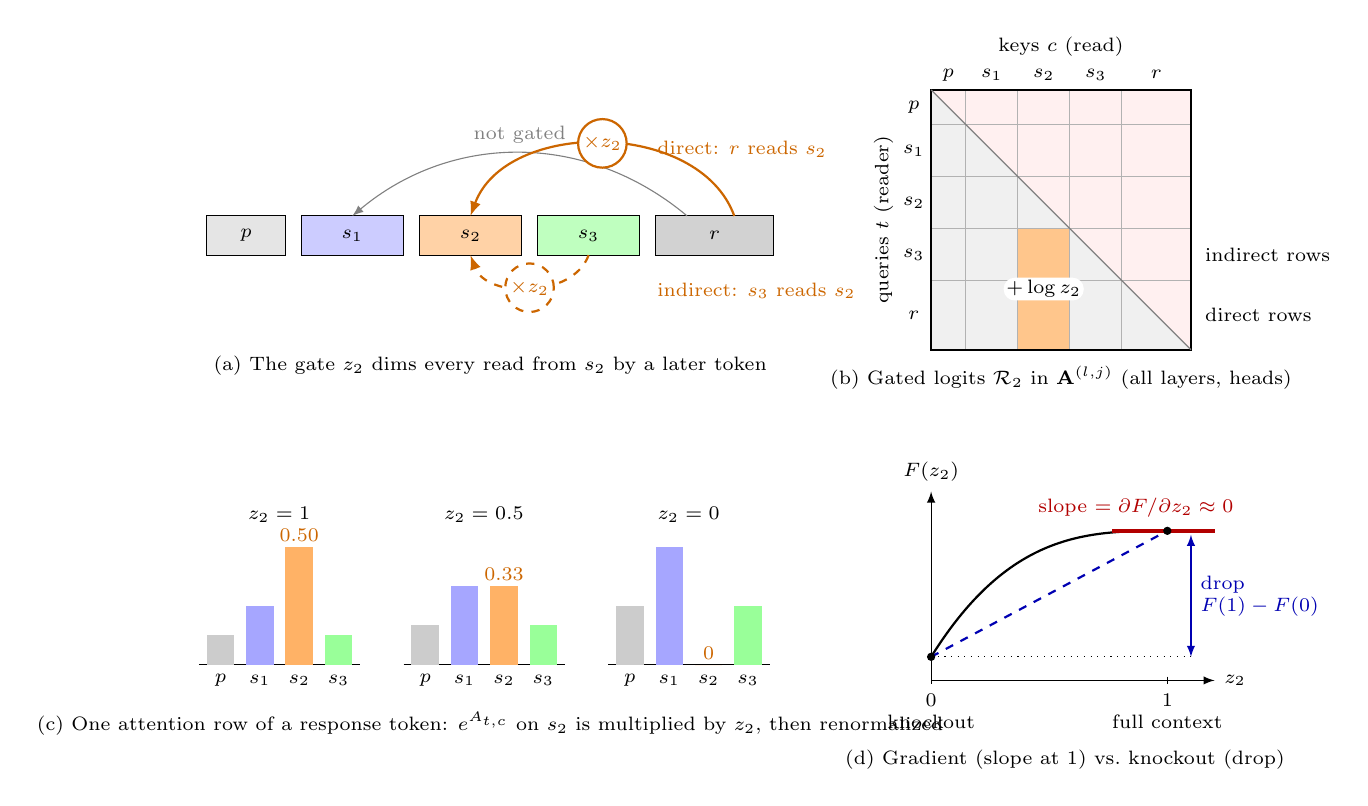
\begin{tikzpicture}[font=\scriptsize, >=latex]
% ================= (a) token sequence =================
\begin{scope}
    \foreach \x/\w/\lab/\col in {0/1.0/p/gray!20, 1.2/1.3/s_1/blue!20, 2.7/1.3/s_2/orange!35, 4.2/1.3/s_3/green!25, 5.7/1.5/r/gray!35}{
        \fill[\col] (\x,0) rectangle ++(\w,0.5);
        \draw (\x,0) rectangle ++(\w,0.5);
        \node at ({\x+\w/2},0.25) {$\lab$};
    }
    % ungated read: response reads s_1
    \draw[->, gray] (6.1,0.5) to[out=140,in=40] node[pos=0.5, above] {not gated} (1.85,0.5);
    % direct gated read: response reads s_2
    \draw[->, thick, orange!80!black] (6.7,0.5) to[out=110,in=70]
        node[pos=0.5, circle, draw, fill=white, inner sep=1pt] {$\times z_2$} (3.35,0.5);
    % indirect gated read: s_3 reads s_2
    \draw[->, thick, dashed, orange!80!black] (4.85,0) to[out=-110,in=-70]
        node[pos=0.5, circle, draw, fill=white, inner sep=1pt] {$\times z_2$} (3.35,0);
    \node[anchor=west, orange!80!black] at (5.6,-0.45) {indirect: $s_3$ reads $s_2$};
    \node[anchor=west, orange!80!black] at (5.6,1.35) {direct: $r$ reads $s_2$};
    \node at (3.6,-1.4) {(a) The gate $z_2$ dims every read from $s_2$ by a later token};
\end{scope}

% ================= (b) attention matrix =================
\begin{scope}[shift={(9.2,-1.2)}, scale=0.55]
    \fill[red!6]   (0,6) -- (6,6) -- (6,0) -- cycle;
    \fill[gray!12] (0,6) -- (0,0) -- (6,0) -- cycle;
    \fill[orange!45] (2.0,0) rectangle (3.2,2.8);
    \foreach \x in {0.8,2.0,3.2,4.4} { \draw[gray!60] (\x,0) -- (\x,6); }
    \foreach \y in {5.2,4.0,2.8,1.6} { \draw[gray!60] (0,\y) -- (6,\y); }
    \draw[thick] (0,0) rectangle (6,6);
    \draw[gray] (0,6) -- (6,0);
    \node at (0.4,6.35) {$p$};   \node at (1.4,6.35) {$s_1$}; \node at (2.6,6.35) {$s_2$};
    \node at (3.8,6.35) {$s_3$}; \node at (5.2,6.35) {$r$};
    \node at (-0.4,5.6) {$p$};   \node at (-0.4,4.6) {$s_1$}; \node at (-0.4,3.4) {$s_2$};
    \node at (-0.4,2.2) {$s_3$}; \node at (-0.4,0.8) {$r$};
    \node at (3,7.0) {keys $c$ (read)};
    \node[rotate=90] at (-1.1,3) {queries $t$ (reader)};
    \node[fill=white, inner sep=1pt, rounded corners] at (2.6,1.4) {$+\log z_2$};
    \node[anchor=west] at (6.1,2.2) {indirect rows};
    \node[anchor=west] at (6.1,0.8) {direct rows};
    \node at (3,-0.65) {(b) Gated logits $\mathcal{R}_2$ in $\mathbf{A}^{(l,j)}$ (all layers, heads)};
\end{scope}

% ================= (c) one attention row =================
\begin{scope}[shift={(0,-5.2)}]
    \foreach \cx/\z/\a/\b/\c/\d/\t in {0/1/0.375/0.75/1.5/0.375/0.50, 2.6/0.5/0.5/1.0/1.0/0.5/0.33, 5.2/0/0.75/1.5/0/0.75/0}{
        \draw (\cx-0.1,0) -- (\cx+1.95,0);
        \fill[gray!40]   (\cx,0)      rectangle ++(0.35,\a);
        \fill[blue!35]   (\cx+0.5,0)  rectangle ++(0.35,\b);
        \fill[orange!60] (\cx+1.0,0)  rectangle ++(0.35,\c);
        \fill[green!40]  (\cx+1.5,0)  rectangle ++(0.35,\d);
        \node at ({\cx+0.175},-0.2) {$p$};
        \node at ({\cx+0.675},-0.2) {$s_1$};
        \node at ({\cx+1.175},-0.2) {$s_2$};
        \node at ({\cx+1.675},-0.2) {$s_3$};
        \node[orange!80!black] at ({\cx+1.175},{\c+0.15}) {\t};
        \node at ({\cx+0.92},1.9) {$z_2 = \z$};
    }
    \node at (3.6,-0.75) {(c) One attention row of a response token: $e^{A_{t,c}}$ on $s_2$ is multiplied by $z_2$, then renormalized};
\end{scope}

% ================= (d) gradient vs. knockout =================
\begin{scope}[shift={(9.2,-5.4)}]
    \draw[->] (0,0) -- (3.6,0) node[right] {$z_2$};
    \draw[->] (0,0) -- (0,2.4) node[above] {$F(z_2)$};
    \draw[thick, domain=0:1, samples=40, smooth] plot ({3*\x},{0.3+1.6*(1-(1-\x)^3)});
    \draw (0,0.05) -- (0,-0.05) node[below, align=center] {$0$\\knockout};
    \draw (3,0.05) -- (3,-0.05) node[below, align=center] {$1$\\full context};
    \draw[dashed, blue!70!black, thick] (0,0.3) -- (3,1.9);
    \draw[dotted] (0,0.3) -- (3.3,0.3);
    \draw[<->, blue!70!black] (3.3,0.3) -- (3.3,1.85) node[midway, right, align=left] {drop\\$F(1)-F(0)$};
    \draw[red!70!black, very thick] (2.3,1.9) -- (3.6,1.9);
    \node[red!70!black, above] at (2.6,1.95) {slope $= \partial F/\partial z_2 \approx 0$};
    \fill (0,0.3) circle (1.5pt);
    \fill (3,1.9) circle (1.5pt);
    \node at (1.7,-1.0) {(d) Gradient (slope at $1$) vs.\ knockout (drop)};
\end{scope}
\end{tikzpicture}%
}
\caption{The snippet gate $z_2$, illustrated for $n = 3$. (a)~The gate multiplies every read from $s_2$ by a later token: directly by the response, and indirectly by later snippets. Reads from other snippets are not affected. (b)~In the logit matrix of every layer and head, the gated entries form the block $\mathcal{R}_2$ (orange) below the diagonal, to which $\log z_2$ is added. The block of $s_2$ reading itself and the masked upper triangle are unchanged. (c)~Effect on one attention row: the share of $s_2$ shrinks as $z_2$ decreases and vanishes at $z_2 = 0$, and the freed mass is redistributed to the other tokens. (d)~The log-likelihood $F(z_2)$ along the gate. The gradient is the slope at full context, which can be close to zero when the model already predicts the response confidently (saturation), even though knocking out $s_2$ causes a large drop. Shapley values of the knockout game average such finite drops over coalitions.}
\label{fig:snippet_gate}
\end{figure}


\paragraph{The attention gradient.}
The following identities are standard consequences of the chain rule and softmax shift invariance.

\begin{lemma}[Gradients through one attention row]\label{lem:attn_grad}
Let $F$ depend on the head output $\mathbf{o}_t$, and let $\boldsymbol{\delta}_t := \partial F / \partial \mathbf{o}_t$. Then, considering only the dependence through row $t$:
\begin{enumerate}
    \item[(i)] $\dfrac{\partial F}{\partial A_{t,c}} = a_{t,c}\, \langle \mathbf{v}_c - \mathbf{o}_t, \boldsymbol{\delta}_t \rangle = a_{t,c} \Big( \dfrac{\partial F}{\partial a_{t,c}} - \sum_{c' \le t} a_{t,c'} \dfrac{\partial F}{\partial a_{t,c'}} \Big)$;
    \item[(ii)] $\sum_{c \le t} \partial F / \partial A_{t,c} = 0$;
    \item[(iii)] $\nabla_{\mathbf{q}_t} F = \frac{1}{\sqrt{d_k}} \sum_{c \le t} \frac{\partial F}{\partial A_{t,c}} \big( \mathbf{k}_c - \bar{\mathbf{k}} \big)$ for \emph{every} vector $\bar{\mathbf{k}} \in \mathbb{R}^{d_k}$;
    \item[(iv)] $\nabla_{\mathbf{v}_c} F = a_{t,c}\, \boldsymbol{\delta}_t$.
\end{enumerate}
\end{lemma}

\begin{proof}
Treating the attention weights as free variables gives $\partial F / \partial a_{t,c} = \langle \mathbf{v}_c, \boldsymbol{\delta}_t \rangle$. The softmax Jacobian is $\partial a_{t,c'} / \partial A_{t,c} = a_{t,c'}(\mathbb{1}[c = c'] - a_{t,c})$, which gives (i). Summing (i) over $c$ gives $\langle \mathbf{o}_t - \mathbf{o}_t, \boldsymbol{\delta}_t \rangle = 0$, which is (ii). For (iii), $\partial A_{t,c} / \partial \mathbf{q}_t = \mathbf{k}_c / \sqrt{d_k}$, and by (ii), subtracting any constant vector $\bar{\mathbf{k}}$ does not change the sum. (iv) follows from $\mathbf{o}_t = \sum_c a_{t,c} \mathbf{v}_c$.
\end{proof}

Identity (i) shows that the logit gradient is the attention $\times$ gradient product used in gradient-weighted attention maps~\cite{chefer2021transformer}, \emph{centered} over the row. Identity (iii) is the gradient counterpart of Proposition~\ref{prop:rcb}(ii): the query gradient is insensitive to a common shift of the keys, so centering keys, as in RCB, loses no gradient information.

\begin{proposition}[Snippet gradient]\label{prop:snippet_gradient}
The derivative of the log-likelihood with respect to the gate of snippet $s_i$ at full context is
\begin{align}\label{eq:snippet_gradient}
    \eta_i := \frac{\partial F}{\partial z_i}\Big|_{\mathbf{z} = \mathbf{1}} = \sum_{l=1}^{L} \sum_{j=1}^{h} \sum_{(t,c) \in \mathcal{R}_i} \underbrace{a^{(l,j)}_{t,c}}_{\text{routing}} \, \underbrace{\big\langle \mathbf{v}^{(l,j)}_c - \mathbf{o}^{(l,j)}_t, \boldsymbol{\delta}^{(l,j)}_t \big\rangle}_{\text{value--error alignment}},
\end{align}
where $\boldsymbol{\delta}^{(l,j)}_t := \partial F / \partial \mathbf{o}^{(l,j)}_t$. It splits into a \emph{direct} part $\eta_i^{\text{dir}}$, collecting the response rows $t \in \mathcal{T}_r$, and an \emph{indirect} part $\eta_i^{\text{ind}}$, collecting the rows of later context tokens, through which information from $s_i$ reaches the response in several hops.
\end{proposition}

\begin{proof}
At $\mathbf{z} = \mathbf{1}$, $\partial / \partial z_i = \partial / \partial \log z_i$. The gate $\log z_i$ enters additively into $A^{(l,j)}_{t,c}$ for every $(l,j)$ and every $(t,c) \in \mathcal{R}_i$. By the multivariable chain rule, $\eta_i$ is the sum of $\partial F / \partial A^{(l,j)}_{t,c}$ over these entries, each given by Lemma~\ref{lem:attn_grad}(i).
\end{proof}

\paragraph{Gradients versus Shapley values.}
Shapley values are themselves integrated gradients, but of a different function and along a full path rather than at a single point. Let 
\begin{align}
    \tilde{v}(\mathbf{x}) := \sum_{S' \subseteq [n]} v(S') \prod_{i \in S'} x_i \prod_{i \notin S'} (1 - x_i)
\end{align} be the multilinear extension of a game $v$ to $[0,1]^n$.

\begin{proposition}[Shapley values as integrated gradients~\cite{owen1972multilinear}]\label{prop:owen}
For every game $v$ and every $i \in [n]$,
\begin{align}
    \phi_i(v) = \int_0^1 \frac{\partial \tilde{v}}{\partial x_i}(s, \dots, s)\, ds.
\end{align}
Consequently, if $F$ is affine on $[0,1]^n$, then $\eta_i = \phi_i(v_{\text{ko}})$ for all $i$.
\end{proposition}

\begin{proof}
$\partial \tilde{v} / \partial x_i (s\mathbf{1}) = \sum_{S' \subseteq [n] \setminus \{i\}} s^{|S'|} (1-s)^{n - 1 - |S'|} \Delta v(S', i)$, and $\int_0^1 s^k (1-s)^{n-1-k} ds = k!(n-1-k)!/n!$, which gives~\eqref{eq:shapley_def}. If $F$ is affine, then $F - F(\mathbf{0})$ is multilinear and agrees with $v_{\text{ko}}$ on the vertices of $[0,1]^n$. Hence it equals $\tilde{v}_{\text{ko}}$, whose partial derivatives are constant and equal to $\eta_i$.
\end{proof}

The snippet gradient $\eta$ and the Shapley value $\boldsymbol{\phi}(v_{\text{ko}})$ therefore differ in two ways. First, $\eta$ is the derivative of the model's own gate extension $F$ at the single point $\mathbf{z} = \mathbf{1}$, whereas $\boldsymbol{\phi}$ averages the derivative of the multilinear extension over the diagonal. The two coincide only if the game has no interactions, so redundancy and complementarity are exactly what first-order attribution misses. Second, gradients \emph{saturate}~\cite{sundararajan2017axiomatic}. The error signal $\boldsymbol{\delta}_t$ is propagated from the output errors $\mathbf{e}_{y_s} - P(\cdot \mid p, S, r_{1:s-1})$ of the response tokens $s \ge t$, whose $\ell_1$-norm is $2(1 - P(y_s \mid p, S, r_{1:s-1}))$. If the model predicts every response token with probability close to one, as is typical for responses it generated itself, then $\eta_i \approx 0$ for every snippet. Removing all snippets, however, may still decrease the likelihood substantially, i.e., $v_{\text{ko}}([n]) \gg 0$. Shapley values are averages of finite differences and do not suffer from this saturation.

\paragraph{What the attention Gram matrices measure.}
By~\eqref{eq:snippet_gradient}, the direct snippet gradient is a sum of products of a routing factor $a_{t,c}$ and a value--error alignment $\langle \mathbf{v}_c - \mathbf{o}_t, \boldsymbol{\delta}_t \rangle$. Post-softmax attention attributions keep only the routing factor. The following proposition shows that the same holds for both GATT constructions, in log scale.

\begin{proposition}[GATT measures log-routing]\label{prop:gatt_log_routing}
For every layer $l$, head $j$, response token $t \in \mathcal{T}_r$ and context tokens $c, c' \in \mathcal{T}_{\text{ctx}}$, we have $A^{(l,j)}_{t,c} - A^{(l,j)}_{t,c'} = \log a^{(l,j)}_{t,c} - \log a^{(l,j)}_{t,c'}$. Consequently:
\begin{enumerate}
    \item[(i)] The unnormalized RCB relevance~\eqref{eq:rcb_block_logit} equals
    \begin{align}
        \sqrt{d_k}\, \operatorname*{mean}_{t \in \mathcal{T}_r} \Big( \operatorname*{mean}_{c \in \mathcal{T}_i^{\text{top}}} \log a^{(l,j)}_{t,c} - \operatorname*{mean}_{c \in \mathcal{T}_{\text{ctx}}} \log a^{(l,j)}_{t,c} \Big),
    \end{align}
    the log-ratio of the geometric-mean attention to the anchor tokens of $s_i$ and to the whole context.
    \item[(ii)] The TCR profile entries are log-excess attention, $f_i(l,j,t) = \frac{1}{k_0} \sum_{c \in \mathcal{T}_i^{\text{top}}(l,j,t)} \big( \log a^{(l,j)}_{t,c} - \log a^{\star}_{l,j,t} \big)^+$, where $a^{\star}_{l,j,t}$ is the attention weight corresponding to the threshold logit $\tau_{l,j,t}$.
\end{enumerate}
\end{proposition}

\begin{proof}
$\log a_{t,c} = A_{t,c} - \log \sum_{c' \le t} e^{A_{t,c'}}$, and the log-partition function is common to all entries of row $t$, so it cancels in differences. Both statements follow by substituting this into~\eqref{eq:rcb_block_logit} and into the definition of $f_i$.
\end{proof}

Both constructions are invariant to row-common shifts, consistent with the zero-sum property of Lemma~\ref{lem:attn_grad}(ii). Gradients, too, only see attention \emph{relative} to the rest of the row. What both constructions discard is the value--error alignment, which has two consequences.
\begin{itemize}
    \item \textbf{Value content.} The alignment can be split as $\langle \mathbf{v}_c, \boldsymbol{\delta}_t \rangle - \langle \mathbf{o}_t, \boldsymbol{\delta}_t \rangle$. The first term is the direct contribution of token $c$. It is small for sink tokens, which attract attention but have value vectors of small norm~\cite{kobayashi2020attention, xiao2024efficient}. The second term is common to the row and scales with attention mass. Routing-only measures cannot separate content from this common term, and the centering in RCB and the thresholding in TCR are partial remedies.
    \item \textbf{Prediction error.} Response tokens that the model predicts confidently induce small gradients but count fully in the uniform averages over $t \in \mathcal{T}_r$ used by RCB and TCR.
\end{itemize}
In exchange, GATT replaces the first-order, additive structure of~\eqref{eq:snippet_gradient} with a cooperative game. Redundant snippets share credit and complementary snippets are both credited, which no single gradient can express (Proposition~\ref{prop:owen}). GATT also uses only the direct rows $t \in \mathcal{T}_r$, so indirect routing through later context tokens ($\eta_i^{\text{ind}}$) is not captured.

\begin{remark}[Error-weighted variants]\label{rem:error_weighted}
The analysis suggests reweighting response tokens by their prediction error, which is available from the forward pass of Section~\ref{subsec:gatt_pipeline} at no extra cost. With $\omega_t := 1 - P(y_t \mid p, S, r_{1:t-1})$ (or the surprisal $-\log P(y_t \mid p, S, r_{1:t-1})$), one replaces the pooled response query of RCB by $\sum_{t \in \mathcal{T}_r} \omega_t \mathbf{q}_t^{(l,j)} / \sum_t \omega_t$, and the TCR profile entries by $\omega_t f_i(l,j,t)$. Since $\boldsymbol{\delta}_t$ aggregates the errors of all later tokens, $\omega_t$ is only a proxy for $\|\boldsymbol{\delta}_t\|$. With one additional backward pass, the exact alignments $\langle \mathbf{v}_c - \mathbf{o}_t, \boldsymbol{\delta}_t \rangle$ can be used instead, e.g., through the profile entries $\big( a_{t,c} \langle \mathbf{v}_c - \mathbf{o}_t, \boldsymbol{\delta}_t \rangle \big)^+$. We leave the empirical evaluation of these variants to future work.
\end{remark}
%%%%%%%%%%%%%%%%%%%%%%%%%%%%%%%%%%%%%%%%%%%%%%%%%%%%%%%%%%%%%%%%%%%%%%%%%%%%%%%%%%%%%%%%%%%%%%%%%%%%%%%%%%%%
%%%%%%%%%%%%%%%%%%%%%%%%%%%%%%%%%%%%%%%%%%%%%%%%%%%%%%%%%%%%%%%%%%%%%%%%%%%%%%%%%%%%%%%%%%%%%%%%%%%%%%%%%%%%
%%%%%%%%%%%%%%%%%%%%%%%%%%%%%%%%%%%%%%%%%%%%%%%%%%%%%%%%%%%%%%%%%%%%%%%%%%%%%%%%%%%%%%%%%%%%%%%%%%%%%%%%%%%%


%%%%%%%%%%%%%%%%%%%%%%%%%%%%%%%%%%%%%%%%%%%%%%%%%%%%%%%%%%%%%%%%%%%%%%%%%%%%%%%%%%%%%%%%%%%%%%%%%%%%%%%%%%%%
% Experiments section for "Attribution for LLMs via Subspace Geometry".
% Generated from the notebooks in
%   //experimental/users/busarobi/attribution/gemma/paper/
% (p1_responses_and_llh_reference, p2_eatt_gecko, p3_gatt_attention,
%  p3b_gatt_ablation, p4_paper_results, p5_baselines); raw results in
%   /cns/ob-d/home/multiverse-ai-crawl-prod/busarobi/gemma4_attribution/paper_v1/
% Requires: \usepackage{booktabs}, \usepackage{graphicx}.
%%%%%%%%%%%%%%%%%%%%%%%%%%%%%%%%%%%%%%%%%%%%%%%%%%%%%%%%%%%%%%%%%%%%%%%%%%%%%%%%%%%%%%%%%%%%%%%%%%%%%%%%%%%%

\section{Experiments}
\label{sec:experiments}

We evaluate the three families of geometric attribution algorithms proposed in this paper. They share the same cooperative game, value functions and link functions, and differ only in where the vectors of the Gram matrix come from:
\begin{itemize}
    \item \textbf{EATT} embeds the snippets and the response with an external text encoder (Section~\ref{subsec:geometric_values});
    \item \textbf{GATT} builds one vector per player from the queries, keys and logits of the LLM, i.e., from \emph{where} the response attends (Section~\ref{sec:attention_gram_attribution});
    \item \textbf{VATT} represents every snippet by the subspace spanned by its value vectors and the response by what it reads from the context, i.e., by \emph{what} the attention moves (Section~\ref{sec:set_embeddings}).
\end{itemize}
All three need at most two LLM forward passes per instance. We compare them with perturbation-based and gradient-based baselines on multi-hop question answering (HotpotQA, 2WikiMultihopQA, MuSiQue), summarization (CNN/DailyMail) and two redundancy variants of HotpotQA, and ask four questions. (i) How closely do they agree with exact likelihood Shapley values~\cite{nematov2025source}? (ii) Do they assign credit to the snippets that actually support the answer? (iii) How do they trade off accuracy against the number of LLM passes, and how does this change with the number of snippets, the task and redundancy among the snippets? (iv) How do the value function, the link function and the hyperparameters affect (i) and (ii)?

\subsection{Experimental Setup}
\label{subsec:exp_setup}

\paragraph{Benchmarks.}
We evaluate on six benchmark settings that differ in the number of snippets, the availability of an exact reference, the presence of supporting-fact labels and the redundancy among snippets (Table~\ref{tab:exp_benchmarks}). All instances are sampled uniformly at random with a fixed seed; every paragraph or sentence is one snippet, prefixed with its title where available.
\begin{itemize}
    \item \textbf{HotpotQA}~\cite{yang2018hotpotqa} (distractor setting, development split), following ContextCite~\cite{cohen2024contextcite}. Every question comes with ten Wikipedia paragraphs, two of which are annotated as \emph{supporting facts}; both are needed for the two-hop reasoning chain. We keep both supporting paragraphs and the first four distractors in their original order ($n = 6$; one instance has only two paragraphs) and truncate each paragraph at $1000$ characters. The distractors are retrieved for lexical overlap with the question and often mention its entities. HotpotQA is the main benchmark ($200$ instances); all ablations in Sections~\ref{subsec:exp_values}--\ref{subsec:exp_cost} use it.
    \item \textbf{2WikiMultihopQA}~\cite{ho2020constructing} (development split, $100$ instances) has the same format with ten paragraphs, of which two to four are supporting facts (compositional, comparison, inference and bridge-comparison questions). We keep all ten paragraphs ($n = 10$), so exact enumeration needs $2^{10} = 1024$ coalitions per instance.
    \item \textbf{MuSiQue}~\cite{trivedi2022musique} (answerable split, development set, $80$ instances) composes two to four single-hop questions into one, so that two to four of its $20$ paragraphs are supporting facts and the others are retrieved distractors. We keep all twenty paragraphs ($n = 20$); exact enumeration ($2^{20}$ coalitions) is infeasible, and this benchmark tests how the methods scale with $n$. Answers are matched against the gold answer and its aliases.
    \item \textbf{CNN/DailyMail}~\cite{nallapati2016abstractive} (version 3.0.0, test split, $100$ articles), the summarization benchmark of ContextCite. The snippets are the first $n = 20$ sentences of each article (articles with fewer than $10$ sentences are skipped), and the instruction asks for a summary of at most three sentences. There are no supporting-fact labels; we evaluate only agreement and ablation faithfulness.
    \item \textbf{Duplicated HotpotQA} and \textbf{paraphrased HotpotQA} ($100$ instances each) test redundancy. We take $100$ of the HotpotQA instances and insert a copy of the first supporting paragraph at a random position that is not adjacent to the original ($n = 7$). In the duplicated variant the copy is verbatim; in the paraphrased variant the model itself rewrites it (\emph{``Paraphrase the following paragraph. Keep every fact, name, date and number, but change the wording and the sentence structure''}, greedy decoding). A faithful attribution method should split the credit between the two copies; leave-one-out cannot, because removing either copy leaves the other in the context.
\end{itemize}

\begin{table}[t]
\centering
\small
\setlength{\tabcolsep}{3pt}
\begin{tabular}{lllrrlrrc}
\toprule
Benchmark & Task & $n$ & Inst. & Supp. & Reference & Coal. & Correct (\%) & $\bar w$ \\
\midrule
HotpotQA & 2-hop QA & 6 & 200 & 2 & exact & 64 & 80.0 & 0.95 \\
2WikiMultihopQA & 2--4-hop QA & 10 & 100 & 2--4 & exact & 1024 & 78.0 & 0.98 \\
MuSiQue & 2--4-hop QA & 20 & 80 & 2--4 & ContextCite-128 & 302 & 55.0 & 0.97 \\
CNN/DailyMail & summarization & $\le 20$ & 100 & -- & ContextCite-128 & 298 & -- & 0.99 \\
HotpotQA + duplicate & 2-hop QA & 7 & 100 & 3 & exact & 127 & 82.0 & 0.96 \\
HotpotQA + paraphrase & 2-hop QA & 7 & 100 & 3 & exact & 127 & 80.0 & 0.96 \\
\bottomrule
\end{tabular}
\caption{Benchmarks. \emph{Supp.:} supporting facts per instance; \emph{Coal.:} mean number of coalitions whose $v_{\text{LL}}$ is evaluated per instance (all $2^n$ for the exact reference; for $n = 20$, the union of the coalitions queried by the baselines, the $128$ reference masks and the $64$ LDS masks); \emph{Correct:} responses that contain the gold answer or an alias; $\bar w$: mean global context weight.}
\label{tab:exp_benchmarks}
\end{table}

\paragraph{Model and responses.}
We use the instruction-tuned Gemma~4 31B dense model~\cite{gemma4}. It has $L = 60$ layers, of which $|\mathcal{L}_{\text{glob}}| = 10$ are global attention layers ($\ell \in \{5, 11, \dots, 59\}$); the remaining layers use a sliding window and cannot route information from distant snippets to the response (Section~\ref{subsec:attention_notation}). Each global layer has $32$ query heads that share $4$ KV heads, with key and value dimension $512$. The prompt $p$ consists of a fixed task instruction (\emph{``Answer the question concisely using only the provided context snippets''} for QA, the summarization instruction above for CNN/DailyMail), the numbered snippets and the question, formatted with the chat template of the model. The response $r$ is generated by the model itself with greedy decoding (at most $64$ tokens for QA and $96$ for summarization), so all methods explain the response the model actually produced. Table~\ref{tab:exp_benchmarks} lists the fraction of responses that contain the normalized gold answer; in most of the other QA instances the model states that the context is insufficient. Because supporting-fact labels strictly apply only to correct answers, we also report all results on the answer-correct instances (Appendix~\ref{app:exp_correct}).

\paragraph{Reference attribution.}
When $n \le 10$ (HotpotQA, 2WikiMultihopQA and both redundancy variants), we evaluate the likelihood game of~\cite{nematov2025source}, $v_{\text{LL}}(S') = \log P(r \mid p, S') - \log P(r \mid p, \emptyset)$, \emph{exactly} on all $2^n$ coalitions and map the exact Shapley vector to the simplex with the rectified link; this reference is free of Monte Carlo noise. On HotpotQA this takes $63.7$ teacher-forced forward passes and $8.3$\,s per instance on $8$ TPU v6e chips. For $n = 20$ (MuSiQue and CNN/DailyMail), we use ContextCite~\cite{cohen2024contextcite} with a high budget of $B = 128$ random ablation masks as the reference, i.e., four times the budget of the ContextCite baseline below, and on MuSiQue we additionally rely on the supporting-fact labels, which do not depend on any reference. Since all methods share the same global context weight $w$ in the final attribution $\boldsymbol{\alpha} = w \cdot g(\boldsymbol{\phi})$ (Definition~\ref{def:attribution_algorithm}), we compare the snippet distributions $g(\boldsymbol{\phi}) \in \Delta^{n-1}$. The responses rely almost entirely on the context ($w \ge 0.95$ on average on every benchmark, Table~\ref{tab:exp_benchmarks}).

\paragraph{Proposed geometric methods.}
Each method below is evaluated with the value functions of Sections~\ref{subsec:geometric_values} and~\ref{subsec:set_values}. Apart from the empty-context pass on $(p, \emptyset, r)$ that is shared by all methods for $w$, GATT and VATT need one teacher-forced pass on $(p, S, r)$, which can be the generation pass itself.
\begin{itemize}
    \item \textbf{EATT (Gecko).} Snippets and response are embedded with the Gecko encoder~\cite{lee2024gecko} ($1$B parameters, $d = 768$) and normalized; the $(n+1) \times (n+1)$ Gram matrix $\mathbf{G}^{+}_{\{[n]\}}$ is formed as in Section~\ref{subsec:geometric_values}.
    \item \textbf{GATT-RCB} and \textbf{GATT-TCR.} The Gram matrices of Section~\ref{subsec:two_grams}, computed from the queries, keys and pre-softmax logits of the $m = 10 \cdot 32$ global heads. Unless stated otherwise, $k_0 = 2$ and $\kappa = 0.9$.
    \item \textbf{VATT.} In every global head $\nu$, snippet $s_i$ is represented by the top-$k$ eigenvectors of its attention-weighted value covariance $\sum_{c \in \mathcal{T}_i} \bar{a}^\nu_c \mathbf{v}^\nu_c \mathbf{v}^{\nu\top}_c$ (rank truncation, Section~\ref{subsec:set_regularization}), and the response by its context read-outs $\mathbf{y}^\nu_t$ (Section~\ref{subsec:vatt}) and, for the principal-angle value functions, by their top-$k_r$ eigenvectors. Heads are combined as a direct sum: $v_{\text{proj}}$ is energy-weighted over heads~\eqref{eq:vatt_proj}, $v_{\text{logvol}}$ is summed, and $v_{\text{vol}}$ and $v_{\text{ent}}$ are averaged over heads (the direct-sum volume is a product of $320$ factors and numerically zero). Unless stated otherwise, $k = k_r = 4$.
\end{itemize}
$v_{\text{logvol}}$ uses $\lambda = 10^{-3}$. For EATT and GATT, Shapley values are estimated with $K = 100$ random permutations ($15$--$30$\,ms per instance on CPU, Section~\ref{subsec:exp_cost}). VATT tabulates its value function on the coalitions it needs, so for $n \le 10$ we compute exact Shapley values and for $n = 20$ we use $K = 50$ permutations. Unless stated otherwise, we report the floor-shifted power link $g^{\text{fl},2}$ of Section~\ref{subsec:contrast_calibration}; Section~\ref{subsec:exp_values} compares it with the rectified link.

\paragraph{Perturbation and gradient baselines.}
Four baselines perturb the snippet set and reuse memoized evaluations of $v_{\text{LL}}(S')$, so their budgets are the exact numbers of distinct LLM forward passes:
\begin{itemize}
    \item \textbf{ContextCite}~\cite{cohen2024contextcite}: sparse linear surrogate (LASSO, penalty $0.01\,\operatorname{sd}(y)$) fitted on $B = 32$ uniform random ablation masks ($25.1$ distinct coalitions on average for $n = 6$).
    \item \textbf{KernelSHAP}~\cite{lundberg2017unified}: least-squares surrogate under the Shapley kernel with the efficiency constraint ($B = 32$: $\emptyset$, $[n]$ and $30$ sampled coalitions).
    \item \textbf{Permutation Shapley (LLH-Perm)}~\cite{castro2009polynomial}: $K$ permutations of $v_{\text{LL}}$ (Lemma~\ref{lemma:unbiased_estimator}); $K = 10$ for $n \le 10$ and $K = 2$ ($2n$ passes) for $n = 20$.
    \item \textbf{Leave-One-Out (LOO)}~\cite{liu2025attribot}: $\phi_i = v_{\text{LL}}([n]) - v_{\text{LL}}([n] \setminus \{i\})$ ($n + 2$ passes including $\emptyset$).
\end{itemize}
Two baselines differentiate $F(\mathbf{x}) = \log P(r \mid \mathbf{x})$ with respect to the token embeddings (Section~\ref{subsec:gradient_view}) and sum token scores within each snippet: \textbf{Gradient $\times$ Input}~\cite{simonyan2014deep} ($1$ forward-backward pass, baseline $\mathbf{x}'$ replaces snippet tokens with the $\langle\text{pad}\rangle$ embedding) and $16$-step \textbf{Integrated Gradients}~\cite{sundararajan2017axiomatic} along $\mathbf{x}' + \alpha(\mathbf{x} - \mathbf{x}')$ ($16$ forward-backward passes). Perturbation and gradient scores are already centered at zero for irrelevant snippets, so we use the rectified link for them (floor-shifting yields similar or lower rank correlation for all six). The direct attention heuristics Citation and Easton V2.1 are evaluated separately in Section~\ref{subsec:exp_citation_easton}.

\paragraph{Metrics.}
All metrics are computed within each instance over its $n$ snippets and averaged over instances, with $95\%$ bootstrap confidence intervals ($2000$ resamples).
\begin{itemize}
    \item \emph{Agreement with the reference:} Pearson $r$, Spearman $\rho$, Kendall $\tau_b$, mean absolute error (MAE, in percentage points) and top-1 agreement.
    \item \emph{Supporting facts:} supporting-fact mass $\sum_{i \in S_{\text{supp}}} g_i(\boldsymbol{\phi})$, AUROC for the binary supporting-fact label, and precision@$k$ (P@$k$) with $k = |S_{\text{supp}}|$ (P@2 on HotpotQA).
    \item \emph{Ablation faithfulness}, which needs no labels and follows ContextCite and AT2~\cite{cohen2024contextcite,cohenwang2025learning}: the \emph{top-$k$ log-probability drop} $v_{\text{LL}}([n]) - v_{\text{LL}}([n] \setminus T_k)$, where $T_k$ holds the $k$ snippets with the largest attribution ($k \in \{1, 2, 3\}$ for $n \le 10$ and $\{1, 3, 5\}$ for $n = 20$; higher is better), and the \emph{linear datamodeling score} (LDS), the Spearman correlation between the additive prediction $\sum_{i \in S'} g_i(\boldsymbol{\phi})$ and $v_{\text{LL}}(S')$ over all $2^n$ coalitions for $n \le 10$ or over $64$ random half-size masks for $n = 20$. Every coalition is scored with an additional teacher-forced pass that is not counted towards the budget of any method.
    \item \emph{Redundancy} (duplicated and paraphrased HotpotQA): the credit on the original and its copy, the \emph{split ratio} $\min(\alpha_o, \alpha_c) / (\alpha_o + \alpha_c)$ ($0.5$ is an even split), and the fraction of instances in which one copy receives less than $1\%$ of their joint credit or both together receive less than $1\%$ of the total.
\end{itemize}

\subsection{Main Results}
\label{subsec:exp_main}

Table~\ref{tab:exp_main} compares the best configuration of every geometric family with all baselines on HotpotQA; Section~\ref{subsec:exp_multi} repeats the comparison on the other benchmarks. The full grid of value functions follows in Section~\ref{subsec:exp_values}.

\begin{table}[t]
\centering
\small
\setlength{\tabcolsep}{2.6pt}
\resizebox{\linewidth}{!}{%
\begin{tabular}{lllcccccccccc}
\toprule
 & & & & \multicolumn{5}{c}{Agreement with Exact LLH-Shapley} & \multicolumn{3}{c}{Supporting facts} \\
\cmidrule(lr){5-9} \cmidrule(lr){10-12}
Method & $v$ & Link & Passes & Pearson $r$ & Spearman $\rho$ & Kendall $\tau$ & MAE (pp) $\downarrow$ & Top-1 (\%) & Mass (\%) & AUROC & P@2 (\%) \\
\midrule
\multicolumn{12}{l}{\emph{Proposed geometric methods (two LLM passes)}} \\
EATT (Gecko) & $v_{\mathrm{logvol}}$ & floor & $2^\dagger$ & 0.75{\scriptsize$\pm$0.05} & 0.68{\scriptsize$\pm$0.03} & 0.59{\scriptsize$\pm$0.03} & 10.3{\scriptsize$\pm$1.2} & 70.0{\scriptsize$\pm$6.2} & \textbf{92.3}{\scriptsize$\pm$1.9} & 0.91{\scriptsize$\pm$0.02} & 83.2{\scriptsize$\pm$3.4} \\
GATT-RCB & $v_{\mathrm{logvol}}$ & floor & 2.0 & 0.72{\scriptsize$\pm$0.05} & 0.60{\scriptsize$\pm$0.04} & 0.51{\scriptsize$\pm$0.04} & 11.7{\scriptsize$\pm$1.3} & 67.0{\scriptsize$\pm$6.5} & 75.4{\scriptsize$\pm$3.1} & 0.83{\scriptsize$\pm$0.03} & 70.8{\scriptsize$\pm$4.0} \\
GATT-TCR & $v_{\mathrm{logvol}}$ & floor & 2.0 & 0.78{\scriptsize$\pm$0.04} & 0.62{\scriptsize$\pm$0.04} & 0.53{\scriptsize$\pm$0.03} & 10.2{\scriptsize$\pm$1.3} & 75.5{\scriptsize$\pm$5.8} & 78.1{\scriptsize$\pm$3.0} & 0.83{\scriptsize$\pm$0.03} & 68.0{\scriptsize$\pm$3.6} \\
VATT & $v_{\mathrm{proj}}$ & floor & 2.0 & \textbf{0.91}{\scriptsize$\pm$0.03} & 0.78{\scriptsize$\pm$0.02} & 0.69{\scriptsize$\pm$0.02} & \textbf{5.8}{\scriptsize$\pm$0.8} & \textbf{82.0}{\scriptsize$\pm$5.2} & 91.5{\scriptsize$\pm$2.0} & \textbf{0.93}{\scriptsize$\pm$0.02} & \textbf{87.8}{\scriptsize$\pm$3.1} \\
VATT & $v_{\mathrm{vol}}$ & rect. & 2.0 & 0.89{\scriptsize$\pm$0.03} & \textbf{0.84}{\scriptsize$\pm$0.03} & \textbf{0.79}{\scriptsize$\pm$0.03} & 6.9{\scriptsize$\pm$0.9} & 78.5{\scriptsize$\pm$5.8} & 91.1{\scriptsize$\pm$2.4} & 0.91{\scriptsize$\pm$0.02} & 84.5{\scriptsize$\pm$3.5} \\
\midrule
\multicolumn{12}{l}{\emph{Gradient and subset-ablation baselines}} \\
Gradient $\times$ Input & $\nabla F$ & rect. & $2.0^\ddagger$ & $-0.01${\scriptsize$\pm$0.06} & $-0.01${\scriptsize$\pm$0.06} & $-0.01${\scriptsize$\pm$0.05} & 26.0{\scriptsize$\pm$1.3} & 18.5{\scriptsize$\pm$5.2} & 30.4{\scriptsize$\pm$4.3} & 0.49{\scriptsize$\pm$0.03} & 30.0{\scriptsize$\pm$4.1} \\
Integrated Gradients (16) & $\nabla F$ & rect. & $17.0^\ddagger$ & 0.07{\scriptsize$\pm$0.06} & 0.10{\scriptsize$\pm$0.06} & 0.09{\scriptsize$\pm$0.06} & 24.1{\scriptsize$\pm$1.1} & 17.0{\scriptsize$\pm$5.0} & 36.8{\scriptsize$\pm$4.5} & 0.54{\scriptsize$\pm$0.03} & 35.2{\scriptsize$\pm$4.1} \\
LOO & $v_{\mathrm{LL}}$ & rect. & 8.0 & 0.97{\scriptsize$\pm$0.01} & 0.77{\scriptsize$\pm$0.03} & 0.71{\scriptsize$\pm$0.03} & 3.3{\scriptsize$\pm$0.5} & 95.5{\scriptsize$\pm$2.8} & 92.9{\scriptsize$\pm$2.4} & 0.90{\scriptsize$\pm$0.02} & 84.5{\scriptsize$\pm$3.4} \\
KernelSHAP (32) & $v_{\mathrm{LL}}$ & rect. & 23.3 & 0.91{\scriptsize$\pm$0.02} & 0.79{\scriptsize$\pm$0.03} & 0.73{\scriptsize$\pm$0.03} & 5.8{\scriptsize$\pm$0.7} & 83.5{\scriptsize$\pm$5.0} & 84.6{\scriptsize$\pm$2.5} & 0.85{\scriptsize$\pm$0.03} & 75.0{\scriptsize$\pm$3.6} \\
ContextCite (32) & $v_{\mathrm{LL}}$ & rect. & 25.1 & 0.99{\scriptsize$\pm$0.01} & 0.90{\scriptsize$\pm$0.02} & 0.86{\scriptsize$\pm$0.02} & 2.5{\scriptsize$\pm$0.3} & 94.5{\scriptsize$\pm$3.2} & 92.0{\scriptsize$\pm$2.1} & 0.90{\scriptsize$\pm$0.02} & 84.0{\scriptsize$\pm$3.5} \\
LLH-Perm ($K=10$) & $v_{\mathrm{LL}}$ & rect. & 34.9 & 0.97{\scriptsize$\pm$0.01} & 0.89{\scriptsize$\pm$0.02} & 0.86{\scriptsize$\pm$0.03} & 2.7{\scriptsize$\pm$0.4} & 88.5{\scriptsize$\pm$4.5} & 93.0{\scriptsize$\pm$2.4} & 0.88{\scriptsize$\pm$0.02} & 80.8{\scriptsize$\pm$3.6} \\
\midrule
Exact LLH-Shapley (ref.) & $v_{\mathrm{LL}}$ & rect. & 63.7 & 1 & 1 & 1 & 0 & 100 & 94.6 & 0.91 & 84.8 \\
Uniform & -- & -- & 0 & -- & -- & -- & 23.7 & 11.5 & 33.7 & 0.50 & 20.5 \\
\bottomrule
\end{tabular}%
}
\caption{Attribution quality on $200$ HotpotQA instances (Gemma~4 31B, $n = 6$ snippets, $2$ supporting facts per instance). Mean over instances $\pm$ half-width of the $95\%$ bootstrap confidence interval. \emph{Passes:} mean distinct LLM passes per instance ($^\dagger$only needed for $w$, plus $n+1$ Gecko encoder calls; $^\ddagger$includes $1$ or $16$ forward-backward passes). VATT uses $k = k_r = 4$. Best entry among the proposed methods is in bold.}
\label{tab:exp_main}
\end{table}

\paragraph{Where the geometry comes from matters most.}
All three families agree with exact likelihood Shapley values far better than uniform attribution (MAE $23.7$\,pp) without ablating a single snippet, but the source of the vectors makes a large difference. EATT and GATT reach Pearson $r = 0.72$--$0.78$ and MAE $10.2$--$11.7$\,pp. VATT reaches $r = 0.91$ and MAE $5.8$\,pp, halving the error of the other two families. With $v_{\text{vol}}$ and the rectified link, it also reaches the highest rank agreement of any two-pass method ($\rho = 0.84$, $\tau = 0.79$). The value vectors are the representations through which the snippets actually influence the response, so a geometry built on them inherits the routing of the model; Gecko cosines describe semantic similarity, and the query--key constructions of GATT describe where the response looks, not what it receives.

\paragraph{Supporting facts.}
EATT and VATT recover the supporting facts as well as the exact reference or better: EATT places $92.3\%$ of the credit on them (AUROC $0.91$, P@2 $83.2\%$), and VATT $91.5\%$ (AUROC $0.93$, P@2 $87.8\%$), compared with $94.6\%$, $0.91$ and $84.8\%$ for exact LLH-Shapley. GATT is weaker at its pre-specified hyperparameters ($75.4$--$78.1\%$ mass, AUROC $0.83$) but closes most of the gap with larger anchor sets (AUROC $0.88$ at $k_0 = 8$, Section~\ref{subsec:exp_sensitivity}). The ordering EATT $>$ GATT follows the similarity structure of the Gram matrices: Gecko cosines between snippets (median $0.47$) separate complementary supporting facts from entity-overlapping distractors more sharply than the nearly orthogonal RCB vectors (median $0.11$) or the background-dominated TCR profiles (median $0.84$).

\paragraph{Accuracy versus cost.}
Figure~\ref{fig:exp_budget} places the methods on the accuracy--cost plane. Methods that query $v_{\text{LL}}(S')$ converge to the reference as their budget grows; ContextCite is the most sample-efficient ($r = 0.86$ at $7.6$ passes, $0.99$ at $25.1$), ahead of LLH-Perm ($0.82$ at $7.0$, $0.97$ at $34.9$) and KernelSHAP ($0.61$ at $7.6$, $0.93$ at $23.0$). LOO reaches $r = 0.97$ at $8$ passes here because the two supporting paragraphs form a \emph{complementary} chain (removing either hop breaks the answer); it assigns zero credit when evidence is duplicated across sources (Section~\ref{sec:related_work}). With two passes, VATT matches the Pearson agreement of KernelSHAP with $23.3$ passes ($r = 0.91$) and exceeds every ablation baseline, including the exact reference, in supporting-fact AUROC ($0.93$ vs.\ $0.85$--$0.91$). EATT and GATT-TCR outperform low-budget KernelSHAP ($B = 8$ and $12$) with $4\times$--$5\times$ fewer passes. Every ablation baseline scales at least linearly with $n$, whereas the geometric methods need two passes for any $n$. The gap to the ablation methods with $25$--$35$ passes ($r \ge 0.97$) remains.

\begin{figure}[t]
\centering
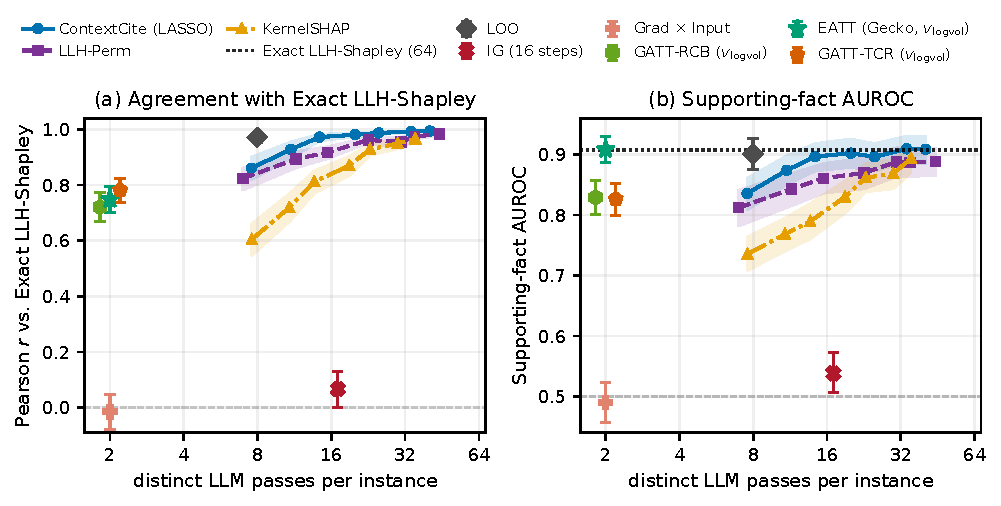
\includegraphics[width=0.95\linewidth]{figures/fig_budget_tradeoff.pdf}
\caption{Attribution accuracy versus mean distinct LLM passes per instance ($200$ HotpotQA instances; bands and error bars are $95\%$ bootstrap confidence intervals). Left: within-instance Pearson $r$ with exact $2^n$ LLH-Shapley. Right: supporting-fact AUROC. VATT ($2$ passes, $r = 0.91$, AUROC $0.93$; Table~\ref{tab:exp_main}) is not drawn.}
\label{fig:exp_budget}
\end{figure}

\paragraph{Gradient baselines fail.}
Both gradient baselines are near chance although they differentiate the exact log-likelihood: Gradient $\times$ Input reaches $r = -0.01$ and AUROC $0.49$, and Integrated Gradients $r = 0.07$ and AUROC $0.54$ at $8.0$\,s per instance. Both failures instantiate the obstructions of Section~\ref{subsec:gradient_view}. At full context, greedy responses have high token probabilities, so the prediction error $\boldsymbol{\delta}_t$ nearly vanishes (Figure~\ref{fig:snippet_gate}(d)): removing the context drops the log-likelihood by a median of $65.9$\,nats, but the $\ell_1$ norm of Gradient $\times$ Input has median $4.1$. Integrated Gradients interpolates token embeddings along a continuous ray through out-of-distribution representations, where attention routing switches abruptly, whereas the Shapley value averages discrete marginal gains along the diagonal of Owen's multilinear extension~\cite{owen1972multilinear} (Proposition~\ref{prop:owen}); its $16$-step quadrature misses the completeness identity by a median relative gap of $2.41$ ($90$th percentile $17.8$).

\subsection{Beyond HotpotQA: More Snippets, Summarization and Redundancy}
\label{subsec:exp_multi}

The HotpotQA instances have $n = 6$ complementary snippets, so exact enumeration and $25$-pass surrogates are affordable and leave-one-out is close to exact. Tables~\ref{tab:exp_multi}--\ref{tab:exp_redundancy} repeat the comparison on settings that stress each of these properties.

\paragraph{More snippets with an exact reference (2WikiMultihopQA).}
With $n = 10$ the exact reference needs $1024$ coalitions per instance, and the conclusions of HotpotQA carry over (Table~\ref{tab:exp_multi}). VATT with $v_{\text{proj}}$ reaches $r = 0.88$ and MAE $4.6$\,pp with two passes, and recovers the supporting facts as well as the exact reference (AUROC $0.99$, P@$k$ $96.0\%$ vs.\ $0.99$ and $94.5\%$); $v_{\text{vol}}$ again gives the best rank agreement of the two-pass methods ($\rho = 0.81$). GATT-TCR improves relative to HotpotQA ($r = 0.78$, AUROC $0.95$), and EATT keeps a high supporting-fact AUROC ($0.95$) despite a lower $r = 0.61$. Among the ablation baselines, KernelSHAP is the first to suffer from the larger game: with the same budget of $32$ samples, its agreement drops from $r = 0.91$ to $0.77$, and its supporting-fact AUROC ($0.89$) falls below that of every VATT variant ($0.98$--$0.99$). ContextCite ($r = 0.97$), LOO ($0.95$, $12$ passes) and LLH-Perm ($0.96$, up to $92$ passes) stay close to the reference, and both gradient baselines stay near chance ($r \le 0.20$).

\paragraph{Twenty snippets (MuSiQue).}
With $n = 20$ snippets, exact enumeration is out of reach, and the reference is ContextCite with $128$ ablations (Table~\ref{tab:exp_multi}, bottom). Because this reference is itself a sparse linear surrogate, its agreement with ContextCite with $32$ ablations ($r = 0.98$) is partly circular; the supporting-fact labels are the reference-free comparison. Here VATT with $v_{\text{logvol}}$ is the best two-pass method ($r = 0.94$, MAE $2.1$\,pp) and recovers the two to four supporting paragraphs among twenty better than the reference itself (AUROC $0.93$ vs.\ $0.90$, P@$k$ $78.5\%$ vs.\ $77.2\%$), and better than every ablation baseline, including LOO with $22$ passes (AUROC $0.89$, P@$k$ $75.8\%$) and ContextCite ($0.87$, $72.9\%$). EATT keeps a high AUROC ($0.91$) and the largest supporting-fact mass of the two-pass methods ($84.4\%$), GATT-TCR reaches $r = 0.87$, and both gradient baselines stay at chance. The fixed-budget surrogates degrade with $n$: KernelSHAP with $32$ samples falls to $r = 0.61$, AUROC $0.73$ and $37.8\%$ supporting-fact mass, and LLH-Perm with $K = 2$ ($40$ passes) to AUROC $0.86$. Rank correlations are low for every method ($\rho \le 0.53$) because most of the twenty snippets receive near-zero credit, so their order is noise. As on CNN/DailyMail, $v_{\text{vol}}$ fails on VATT with many snippets ($r = 0.31$), whereas $v_{\text{logvol}}$ improves over $v_{\text{proj}}$ ($r = 0.94$ vs.\ $0.92$, AUROC $0.93$ vs.\ $0.90$). Scoring the $302$ coalitions per instance needed for the reference, the baselines and the LDS took $120$\,s per instance; the GATT forward pass took $2.6$\,s.

\paragraph{Summarization (CNN/DailyMail).}
Summaries draw on many sentences at once, and the reference is spread accordingly (uniform attribution has MAE $6.8$\,pp). VATT with $v_{\text{logvol}}$ agrees best among the two-pass methods ($r = 0.89$, $\rho = 0.75$, MAE $2.5$\,pp, LDS $0.87$), on par with LLH-Perm with $K = 2$ ($r = 0.88$, LDS $0.87$, up to $40$ passes) and well ahead of KernelSHAP ($r = 0.67$, LDS $0.74$); ContextCite ($r = 0.94$, LDS $0.91$) and LOO ($r = 0.91$, LDS $0.89$, $22$ passes) remain the most faithful. In contrast to QA, $v_{\text{vol}}$ collapses on VATT ($r = 0.43$): summary sentences read from many overlapping value subspaces, and the volume difference, which penalizes every shared direction, assigns non-positive credit to most of them. The log-volume, whose marginal gains stay non-negative~\eqref{eq:marginal_logvol}, is the robust choice when many snippets contribute. Removing the five sentences ranked highest by VATT lowers the log-likelihood by $301$\,nats ($v_{\text{logvol}}$; $314$ for the reference and $304$ for ContextCite), against $251$ for the first five sentences of the article (Table~\ref{tab:exp_faithfulness}).

\paragraph{Ablation faithfulness.}
Table~\ref{tab:exp_faithfulness} reports the label-free metrics of ContextCite and AT2. They reproduce the ordering of the agreement metrics on every benchmark. VATT reaches LDS $0.79$--$0.87$ on all four benchmarks, with top-$1$ drops within $3$--$7$\,nats of the reference on the three QA benchmarks, ahead of EATT and GATT and of KernelSHAP with $32$ samples for $n \ge 10$, while the gradient baselines stay close to or below uniform attribution (LDS $0.23$--$0.42$ vs.\ $0.37$--$0.54$). The surrogates that fit $v_{\text{LL}}$ directly (ContextCite, LOO, LLH-Perm) achieve the highest LDS, as expected from a metric defined on $v_{\text{LL}}$ itself.

\paragraph{Redundant snippets.}
Table~\ref{tab:exp_redundancy} confirms the structural weakness of leave-one-out. When the first supporting paragraph appears twice, removing either copy leaves the other in place, so LOO assigns less than $1\%$ of the credit to both copies together in $51\%$ of the instances (verbatim) and $35\%$ (paraphrase); the pair receives $12.2\%$ and $28.2\%$ of the credit, against $47.2\%$ and $46.7\%$ for the exact reference, and the agreement of LOO with the reference falls from $r = 0.97$ on the original instances to $0.66$ and $0.83$ (AUROC $0.69$ and $0.76$). The Shapley-based methods share the credit: the exact reference splits it with ratio $0.39$ (verbatim) and $0.30$ (paraphrase), and VATT with $v_{\text{proj}}$ places $51.6\%$ and $51.8\%$ on the pair with split ratios $0.35$ and $0.36$, keeping $r = 0.84$ and AUROC $0.91$ on both variants. EATT behaves similarly (split $0.39$ and $0.31$). The volume difference splits less evenly ($0.20$--$0.24$), because once one copy is in the coalition the other adds no new volume. A paraphrase is only partially redundant for the model: the reference splits less evenly than for a verbatim copy, and LOO zeroes the pair less often.

\begin{table}[t]
\centering
\small
\setlength{\tabcolsep}{2.6pt}
\resizebox{\linewidth}{!}{%
\begin{tabular}{lllcccccccc}
\toprule
 & & & & \multicolumn{4}{c}{Agreement with reference} & \multicolumn{3}{c}{Supporting facts} \\
\cmidrule(lr){5-8} \cmidrule(lr){9-11}
Method & $v$ & Link & Passes & Pearson $r$ & Spearman $\rho$ & MAE (pp) $\downarrow$ & Top-1 (\%) & Mass (\%) & AUROC & P@$k$ (\%) \\
\midrule
\multicolumn{11}{l}{\textbf{2WikiMultihopQA (exact reference)} ($n = 10$, 100 instances)} \\
EATT (Gecko) & $v_{\mathrm{logvol}}$ & floor & $2^\dagger$ & 0.61{\scriptsize$\pm$0.06} & 0.65{\scriptsize$\pm$0.03} & 9.0{\scriptsize$\pm$0.9} & 39.0{\scriptsize$\pm$9.5} & 89.5{\scriptsize$\pm$3.4} & 0.95{\scriptsize$\pm$0.02} & 85.2{\scriptsize$\pm$4.9} \\
GATT-RCB & $v_{\mathrm{logvol}}$ & floor & 2 & 0.63{\scriptsize$\pm$0.06} & 0.51{\scriptsize$\pm$0.05} & 8.7{\scriptsize$\pm$0.6} & 48.0{\scriptsize$\pm$9.5} & 64.1{\scriptsize$\pm$4.5} & 0.87{\scriptsize$\pm$0.03} & 68.5{\scriptsize$\pm$6.1} \\
GATT-TCR & $v_{\mathrm{logvol}}$ & floor & 2 & 0.78{\scriptsize$\pm$0.05} & 0.63{\scriptsize$\pm$0.04} & 6.3{\scriptsize$\pm$0.6} & 59.0{\scriptsize$\pm$9.5} & 81.1{\scriptsize$\pm$3.5} & 0.95{\scriptsize$\pm$0.02} & 84.5{\scriptsize$\pm$4.6} \\
VATT & $v_{\mathrm{proj}}$ & floor & 2 & 0.88{\scriptsize$\pm$0.03} & 0.71{\scriptsize$\pm$0.03} & 4.6{\scriptsize$\pm$0.4} & 64.0{\scriptsize$\pm$9.5} & 88.4{\scriptsize$\pm$2.4} & 0.99{\scriptsize$\pm$0.01} & 96.0{\scriptsize$\pm$3.0} \\
VATT & $v_{\mathrm{logvol}}$ & floor & 2 & 0.88{\scriptsize$\pm$0.03} & 0.69{\scriptsize$\pm$0.03} & 4.5{\scriptsize$\pm$0.5} & 65.0{\scriptsize$\pm$9.5} & 87.6{\scriptsize$\pm$2.3} & 0.99{\scriptsize$\pm$0.01} & 96.0{\scriptsize$\pm$2.4} \\
VATT & $v_{\mathrm{vol}}$ & rect. & 2 & 0.86{\scriptsize$\pm$0.03} & 0.81{\scriptsize$\pm$0.04} & 4.6{\scriptsize$\pm$0.5} & 59.0{\scriptsize$\pm$9.5} & 89.4{\scriptsize$\pm$2.9} & 0.98{\scriptsize$\pm$0.01} & 93.8{\scriptsize$\pm$3.3} \\
\addlinespace[2pt]
Gradient $\times$ Input & $\nabla F$ & rect. & $2^\ddagger$ & 0.10{\scriptsize$\pm$0.08} & 0.02{\scriptsize$\pm$0.07} & 14.8{\scriptsize$\pm$0.9} & 15.0{\scriptsize$\pm$7.0} & 31.0{\scriptsize$\pm$5.6} & 0.52{\scriptsize$\pm$0.05} & 32.0{\scriptsize$\pm$5.5} \\
Integrated Gradients (16) & $\nabla F$ & rect. & $17^\ddagger$ & 0.20{\scriptsize$\pm$0.08} & 0.16{\scriptsize$\pm$0.07} & 13.9{\scriptsize$\pm$0.9} & 20.0{\scriptsize$\pm$7.5} & 36.1{\scriptsize$\pm$5.9} & 0.62{\scriptsize$\pm$0.05} & 36.2{\scriptsize$\pm$6.5} \\
LOO & $v_{\mathrm{LL}}$ & rect. & 12 & 0.95{\scriptsize$\pm$0.03} & 0.73{\scriptsize$\pm$0.03} & 2.8{\scriptsize$\pm$0.5} & 83.0{\scriptsize$\pm$7.5} & 92.3{\scriptsize$\pm$2.9} & 0.98{\scriptsize$\pm$0.02} & 95.2{\scriptsize$\pm$3.0} \\
KernelSHAP (32) & $v_{\mathrm{LL}}$ & rect. & $\le 32$ & 0.77{\scriptsize$\pm$0.06} & 0.63{\scriptsize$\pm$0.05} & 6.4{\scriptsize$\pm$0.7} & 61.0{\scriptsize$\pm$9.5} & 70.0{\scriptsize$\pm$4.2} & 0.89{\scriptsize$\pm$0.03} & 73.5{\scriptsize$\pm$5.8} \\
ContextCite (32) & $v_{\mathrm{LL}}$ & rect. & $\le 32$ & 0.97{\scriptsize$\pm$0.02} & 0.78{\scriptsize$\pm$0.03} & 2.2{\scriptsize$\pm$0.3} & 88.0{\scriptsize$\pm$6.5} & 87.5{\scriptsize$\pm$3.0} & 0.97{\scriptsize$\pm$0.02} & 93.8{\scriptsize$\pm$3.3} \\
LLH-Perm ($K=10$) & $v_{\mathrm{LL}}$ & rect. & $\le 92$ & 0.96{\scriptsize$\pm$0.02} & 0.83{\scriptsize$\pm$0.03} & 2.0{\scriptsize$\pm$0.3} & 84.0{\scriptsize$\pm$7.5} & 91.7{\scriptsize$\pm$2.7} & 0.97{\scriptsize$\pm$0.01} & 92.8{\scriptsize$\pm$3.4} \\
Exact LLH-Shapley (ref.) & $v_{\mathrm{LL}}$ & rect. & 1024 & 1 & 1 & 0 & 100 & 94.1 & 0.99 & 94.5 \\
Uniform & -- & -- & 0 & -- & -- & 14.5 & 5.0 & 24.0 & 0.50 & 26.0 \\
\midrule
\multicolumn{11}{l}{\textbf{MuSiQue (sampled reference)} ($n = 20$, 80 instances)} \\
EATT (Gecko) & $v_{\mathrm{logvol}}$ & floor & $2^\dagger$ & 0.69{\scriptsize$\pm$0.07} & 0.38{\scriptsize$\pm$0.04} & 4.2{\scriptsize$\pm$0.6} & 51.2{\scriptsize$\pm$11.2} & 84.4{\scriptsize$\pm$5.0} & 0.91{\scriptsize$\pm$0.03} & 72.8{\scriptsize$\pm$5.8} \\
GATT-RCB & $v_{\mathrm{logvol}}$ & floor & 2 & 0.68{\scriptsize$\pm$0.08} & 0.32{\scriptsize$\pm$0.04} & 4.6{\scriptsize$\pm$0.5} & 55.0{\scriptsize$\pm$10.6} & 54.1{\scriptsize$\pm$5.4} & 0.81{\scriptsize$\pm$0.04} & 57.1{\scriptsize$\pm$6.6} \\
GATT-TCR & $v_{\mathrm{logvol}}$ & floor & 2 & 0.87{\scriptsize$\pm$0.05} & 0.35{\scriptsize$\pm$0.04} & 3.2{\scriptsize$\pm$0.4} & 77.5{\scriptsize$\pm$8.8} & 65.9{\scriptsize$\pm$4.3} & 0.86{\scriptsize$\pm$0.04} & 66.5{\scriptsize$\pm$5.5} \\
VATT & $v_{\mathrm{proj}}$ & floor & 2 & 0.91{\scriptsize$\pm$0.03} & 0.38{\scriptsize$\pm$0.03} & 2.9{\scriptsize$\pm$0.3} & 85.0{\scriptsize$\pm$8.1} & 70.1{\scriptsize$\pm$4.2} & 0.90{\scriptsize$\pm$0.03} & 73.5{\scriptsize$\pm$5.6} \\
VATT & $v_{\mathrm{logvol}}$ & floor & 2 & 0.94{\scriptsize$\pm$0.03} & 0.42{\scriptsize$\pm$0.04} & 2.1{\scriptsize$\pm$0.3} & 85.0{\scriptsize$\pm$7.5} & 81.2{\scriptsize$\pm$3.8} & 0.93{\scriptsize$\pm$0.03} & 78.5{\scriptsize$\pm$5.3} \\
VATT & $v_{\mathrm{vol}}$ & rect. & 2 & 0.31{\scriptsize$\pm$0.07} & 0.23{\scriptsize$\pm$0.05} & 7.2{\scriptsize$\pm$0.3} & 23.8{\scriptsize$\pm$9.4} & 28.1{\scriptsize$\pm$3.4} & 0.68{\scriptsize$\pm$0.04} & 31.1{\scriptsize$\pm$5.2} \\
\addlinespace[2pt]
Gradient $\times$ Input & $\nabla F$ & rect. & $2^\ddagger$ & 0.05{\scriptsize$\pm$0.06} & 0.03{\scriptsize$\pm$0.05} & 8.5{\scriptsize$\pm$0.3} & 7.5{\scriptsize$\pm$5.6} & 13.9{\scriptsize$\pm$3.6} & 0.51{\scriptsize$\pm$0.04} & 13.6{\scriptsize$\pm$4.5} \\
Integrated Gradients (16) & $\nabla F$ & rect. & $17^\ddagger$ & 0.07{\scriptsize$\pm$0.06} & 0.04{\scriptsize$\pm$0.05} & 8.6{\scriptsize$\pm$0.3} & 13.8{\scriptsize$\pm$7.5} & 15.4{\scriptsize$\pm$3.9} & 0.56{\scriptsize$\pm$0.04} & 14.5{\scriptsize$\pm$4.6} \\
LOO & $v_{\mathrm{LL}}$ & rect. & 22 & 0.95{\scriptsize$\pm$0.03} & 0.42{\scriptsize$\pm$0.04} & 1.9{\scriptsize$\pm$0.4} & 91.2{\scriptsize$\pm$5.6} & 80.6{\scriptsize$\pm$5.3} & 0.89{\scriptsize$\pm$0.03} & 75.8{\scriptsize$\pm$5.9} \\
KernelSHAP (32) & $v_{\mathrm{LL}}$ & rect. & $\le 32$ & 0.61{\scriptsize$\pm$0.06} & 0.27{\scriptsize$\pm$0.04} & 5.8{\scriptsize$\pm$0.3} & 53.8{\scriptsize$\pm$10.0} & 37.8{\scriptsize$\pm$4.0} & 0.73{\scriptsize$\pm$0.04} & 43.5{\scriptsize$\pm$5.8} \\
ContextCite (32) & $v_{\mathrm{LL}}$ & rect. & $\le 32$ & 0.98{\scriptsize$\pm$0.01} & 0.53{\scriptsize$\pm$0.04} & 1.2{\scriptsize$\pm$0.2} & 96.2{\scriptsize$\pm$4.4} & 82.6{\scriptsize$\pm$4.2} & 0.87{\scriptsize$\pm$0.03} & 72.9{\scriptsize$\pm$5.6} \\
LLH-Perm ($K=2$) & $v_{\mathrm{LL}}$ & rect. & $\le 40$ & 0.92{\scriptsize$\pm$0.03} & 0.44{\scriptsize$\pm$0.04} & 2.3{\scriptsize$\pm$0.3} & 86.2{\scriptsize$\pm$7.5} & 74.7{\scriptsize$\pm$4.5} & 0.86{\scriptsize$\pm$0.04} & 70.8{\scriptsize$\pm$6.1} \\
ContextCite (128, ref.) & $v_{\mathrm{LL}}$ & rect. & $\le 128$ & 1 & 1 & 0 & 100 & 85.8 & 0.90 & 77.2 \\
Uniform & -- & -- & 0 & -- & -- & 8.1 & 3.8 & 12.9 & 0.50 & 13.1 \\
\bottomrule
\end{tabular}%
}
\caption{Attribution quality beyond HotpotQA. Mean over instances $\pm$ half-width of the $95\%$ bootstrap confidence interval. 2WikiMultihopQA uses the exact $2^{10}$ LLH-Shapley reference; MuSiQue ($n = 20$) uses $128$-mask ContextCite, so the supporting-fact columns are the reference-free comparison. P@$k$ uses $k = |S_{\text{supp}}|$. \emph{Passes:} distinct LLM passes per instance ($^\dagger$only for $w$, plus $n+1$ encoder calls; $^\ddagger$forward-backward passes).}
\label{tab:exp_multi}
\end{table}

\begin{table}[t]
\centering
\small
\setlength{\tabcolsep}{3pt}
\resizebox{\linewidth}{!}{%
\begin{tabular}{lcccccccccccc}
\toprule
 & \multicolumn{3}{c}{HotpotQA ($n{=}6$)} & \multicolumn{3}{c}{2Wiki ($n{=}10$)} & \multicolumn{3}{c}{MuSiQue ($n{=}20$)} & \multicolumn{3}{c}{CNN/DM ($n{=}20$)} \\
\cmidrule(lr){2-4} \cmidrule(lr){5-7} \cmidrule(lr){8-10} \cmidrule(lr){11-13}
Method & LDS & drop@1 & drop@3 & LDS & drop@1 & drop@3 & LDS & drop@1 & drop@5 & LDS & drop@1 & drop@5 \\
\midrule
EATT (Gecko) $v_{\mathrm{logvol}}$ & 0.73 & 65.7 & 88.4 & 0.70 & 53.3 & 100.0 & 0.71 & 72.7 & 116.0 & 0.66 & 81.5 & 242.5 \\
GATT-TCR $v_{\mathrm{logvol}}$ & 0.72 & 67.2 & 87.7 & 0.77 & 66.0 & 102.1 & 0.79 & 87.5 & 116.3 & 0.81 & 110.7 & 274.4 \\
VATT $v_{\mathrm{proj}}$ & 0.79 & 72.5 & 92.1 & 0.83 & 69.8 & 107.3 & 0.83 & 92.5 & 118.0 & 0.85 & 109.4 & 289.8 \\
VATT $v_{\mathrm{logvol}}$ & 0.79 & 71.4 & 91.2 & 0.82 & 70.2 & 105.6 & 0.84 & 92.5 & 118.2 & 0.87 & 114.7 & 301.0 \\
VATT $v_{\mathrm{vol}}$ & 0.80 & 70.9 & 91.2 & 0.82 & 70.8 & 108.0 & 0.45 & 33.8 & 86.9 & 0.60 & 58.6 & 207.0 \\
\midrule
Gradient $\times$ Input & 0.27 & 17.3 & 47.7 & 0.31 & 23.4 & 47.3 & 0.23 & 13.1 & 44.1 & 0.29 & 19.7 & 117.4 \\
Integrated Gradients (16) & 0.34 & 21.9 & 58.4 & 0.37 & 31.0 & 60.1 & 0.25 & 18.7 & 53.5 & 0.42 & 34.8 & 152.9 \\
LOO & 0.84 & 76.9 & 88.7 & 0.86 & 78.6 & 106.0 & 0.85 & 95.7 & 118.1 & 0.88 & 132.6 & 292.3 \\
KernelSHAP (32) & 0.80 & 72.0 & 91.5 & 0.75 & 66.2 & 99.8 & 0.62 & 66.8 & 109.3 & 0.74 & 95.5 & 258.8 \\
ContextCite (32) & 0.86 & 76.1 & 93.8 & 0.88 & 76.8 & 109.0 & 0.88 & 95.1 & 124.4 & 0.91 & 122.6 & 304.1 \\
LLH-Perm ($K = 10$ / $2$) & 0.84 & 75.4 & 92.4 & 0.87 & 77.3 & 109.7 & 0.84 & 92.9 & 118.8 & 0.87 & 114.6 & 292.6 \\
\midrule
Reference & 0.87 & 76.5 & 93.7 & 0.90 & 77.2 & 110.6 & 0.90 & 95.3 & 124.4 & 0.93 & 126.2 & 313.9 \\
Uniform & 0.45 & 11.8 & 34.8 & 0.44 & 17.6 & 48.1 & 0.37 & 12.5 & 100.0 & 0.54 & 64.1 & 250.5 \\
\bottomrule
\end{tabular}%
}
\caption{Ablation faithfulness without labels. LDS: Spearman correlation between $\sum_{i \in S'} g_i(\boldsymbol{\phi})$ and $v_{\text{LL}}(S')$ over all coalitions ($n \le 10$) or $64$ random masks ($n = 20$). drop@$k$: log-likelihood drop (nats) when the $k$ highest-attributed snippets are removed; higher is better. \emph{Uniform} breaks ties by position, i.e., it removes the first $k$ snippets. Default link of each method as in Table~\ref{tab:exp_main}.}
\label{tab:exp_faithfulness}
\end{table}

\begin{table}[t]
\centering
\small
\setlength{\tabcolsep}{3pt}
\resizebox{\linewidth}{!}{%
\begin{tabular}{lcccccccccc}
\toprule
 & \multicolumn{5}{c}{Duplicated copy} & \multicolumn{5}{c}{Paraphrased copy} \\
\cmidrule(lr){2-6} \cmidrule(lr){7-11}
Method & Pair (\%) & Split & Both $\approx 0$ (\%) & $r$ & AUROC & Pair (\%) & Split & Both $\approx 0$ (\%) & $r$ & AUROC \\
\midrule
EATT (Gecko) $v_{\mathrm{logvol}}$ & 40.6 & 0.39 & 6 & 0.70 & 0.89 & 45.8 & 0.31 & 7 & 0.66 & 0.88 \\
GATT-TCR $v_{\mathrm{logvol}}$ & 42.2 & 0.24 & 6 & 0.72 & 0.77 & 43.4 & 0.25 & 7 & 0.73 & 0.76 \\
VATT $v_{\mathrm{proj}}$ & 51.6 & 0.35 & 8 & 0.84 & 0.91 & 51.8 & 0.36 & 9 & 0.84 & 0.91 \\
VATT $v_{\mathrm{logvol}}$ & 50.0 & 0.28 & 7 & 0.81 & 0.89 & 50.1 & 0.31 & 8 & 0.83 & 0.88 \\
VATT $v_{\mathrm{vol}}$ & 43.9 & 0.20 & 15 & 0.81 & 0.85 & 48.8 & 0.24 & 12 & 0.82 & 0.87 \\
\midrule
Gradient $\times$ Input & 29.8 & 0.05 & 27 & 0.03 & 0.51 & 29.3 & 0.07 & 22 & 0.03 & 0.51 \\
Integrated Gradients (16) & 23.4 & 0.07 & 25 & 0.03 & 0.49 & 25.5 & 0.07 & 24 & 0.02 & 0.51 \\
LOO & 12.2 & 0.15 & 51 & 0.66 & 0.69 & 28.2 & 0.11 & 35 & 0.83 & 0.76 \\
KernelSHAP (32) & 45.1 & 0.24 & 12 & 0.87 & 0.82 & 45.7 & 0.22 & 12 & 0.88 & 0.82 \\
ContextCite (32) & 45.0 & 0.36 & 8 & 0.96 & 0.90 & 46.1 & 0.30 & 11 & 0.97 & 0.89 \\
LLH-Perm ($K = 10$) & 48.8 & 0.25 & 10 & 0.94 & 0.89 & 48.3 & 0.21 & 16 & 0.94 & 0.87 \\
\midrule
Exact LLH-Shapley (ref.) & 47.2 & 0.39 & 19 & 1 & 0.89 & 46.7 & 0.30 & 22 & 1 & 0.88 \\
\bottomrule
\end{tabular}%
}
\caption{Redundancy test on $100$ HotpotQA instances with a verbatim (left) or model-paraphrased (right) copy of the first supporting paragraph ($n = 7$). \emph{Pair:} credit on the original and the copy together; \emph{Split:} $\min(\alpha_o, \alpha_c)/(\alpha_o + \alpha_c)$, $0.5$ is an even split; \emph{Both $\approx 0$:} fraction of instances where the two copies together receive less than $1\%$ of the credit. $r$ and AUROC as in Table~\ref{tab:exp_main}.}
\label{tab:exp_redundancy}
\end{table}

\subsection{Value Functions and Link Functions}
\label{subsec:exp_values}

Table~\ref{tab:exp_values} reports every value function for every family, and Table~\ref{tab:exp_links} isolates the effect of the link function.

\begin{table}[t]
\centering
\small
\setlength{\tabcolsep}{3.0pt}
\resizebox{\linewidth}{!}{%
\begin{tabular}{llcccccccc}
\toprule
 & & \multicolumn{5}{c}{Agreement with Exact LLH-Shapley} & \multicolumn{3}{c}{Supporting facts} \\
\cmidrule(lr){3-7} \cmidrule(lr){8-10}
Method & $v$ & Pearson $r$ & Spearman $\rho$ & Kendall $\tau$ & MAE (pp) $\downarrow$ & Top-1 (\%) & Mass (\%) & AUROC & P@2 (\%) \\
\midrule
EATT (Gecko) & $v_{\mathrm{vol}}$ & 0.75{\scriptsize$\pm$0.05} & 0.61{\scriptsize$\pm$0.04} & 0.53{\scriptsize$\pm$0.04} & 10.5{\scriptsize$\pm$1.1} & 70.5{\scriptsize$\pm$6.2} & 89.3{\scriptsize$\pm$2.1} & 0.87{\scriptsize$\pm$0.03} & 77.5{\scriptsize$\pm$3.6} \\
EATT (Gecko) & $v_{\mathrm{logvol}}$ & 0.75{\scriptsize$\pm$0.05} & 0.68{\scriptsize$\pm$0.03} & 0.59{\scriptsize$\pm$0.03} & 10.3{\scriptsize$\pm$1.2} & 70.0{\scriptsize$\pm$6.2} & 92.3{\scriptsize$\pm$1.9} & 0.91{\scriptsize$\pm$0.02} & 83.2{\scriptsize$\pm$3.4} \\
EATT (Gecko) & $v_{\mathrm{ent}}$ & 0.74{\scriptsize$\pm$0.05} & 0.65{\scriptsize$\pm$0.04} & 0.57{\scriptsize$\pm$0.03} & 10.6{\scriptsize$\pm$1.1} & 66.0{\scriptsize$\pm$6.5} & 86.5{\scriptsize$\pm$2.2} & 0.89{\scriptsize$\pm$0.02} & 79.0{\scriptsize$\pm$3.6} \\
\addlinespace[2pt]
GATT-RCB & $v_{\mathrm{vol}}$ & 0.69{\scriptsize$\pm$0.05} & 0.57{\scriptsize$\pm$0.05} & 0.49{\scriptsize$\pm$0.04} & 12.4{\scriptsize$\pm$1.4} & 65.5{\scriptsize$\pm$6.5} & 73.5{\scriptsize$\pm$3.1} & 0.81{\scriptsize$\pm$0.03} & 68.5{\scriptsize$\pm$3.9} \\
GATT-RCB & $v_{\mathrm{logvol}}$ & 0.72{\scriptsize$\pm$0.05} & 0.60{\scriptsize$\pm$0.04} & 0.51{\scriptsize$\pm$0.04} & 11.7{\scriptsize$\pm$1.3} & 67.0{\scriptsize$\pm$6.5} & 75.4{\scriptsize$\pm$3.1} & 0.83{\scriptsize$\pm$0.03} & 70.8{\scriptsize$\pm$4.0} \\
GATT-RCB & $v_{\mathrm{ent}}$ & 0.73{\scriptsize$\pm$0.05} & 0.60{\scriptsize$\pm$0.04} & 0.52{\scriptsize$\pm$0.04} & 12.0{\scriptsize$\pm$1.3} & 67.5{\scriptsize$\pm$6.5} & 72.4{\scriptsize$\pm$2.9} & 0.83{\scriptsize$\pm$0.03} & 68.8{\scriptsize$\pm$4.0} \\
\addlinespace[2pt]
GATT-TCR & $v_{\mathrm{vol}}$ & 0.27{\scriptsize$\pm$0.06} & 0.33{\scriptsize$\pm$0.04} & 0.28{\scriptsize$\pm$0.04} & 20.7{\scriptsize$\pm$1.3} & 23.5{\scriptsize$\pm$5.8} & 44.6{\scriptsize$\pm$3.9} & 0.65{\scriptsize$\pm$0.03} & 51.2{\scriptsize$\pm$3.0} \\
GATT-TCR & $v_{\mathrm{logvol}}$ & 0.78{\scriptsize$\pm$0.04} & 0.62{\scriptsize$\pm$0.04} & 0.53{\scriptsize$\pm$0.03} & 10.2{\scriptsize$\pm$1.3} & 75.5{\scriptsize$\pm$5.8} & 78.1{\scriptsize$\pm$3.0} & 0.83{\scriptsize$\pm$0.03} & 68.0{\scriptsize$\pm$3.6} \\
GATT-TCR & $v_{\mathrm{ent}}$ & 0.29{\scriptsize$\pm$0.06} & 0.34{\scriptsize$\pm$0.04} & 0.29{\scriptsize$\pm$0.04} & 20.4{\scriptsize$\pm$1.3} & 25.0{\scriptsize$\pm$6.0} & 44.3{\scriptsize$\pm$3.6} & 0.66{\scriptsize$\pm$0.03} & 49.8{\scriptsize$\pm$3.4} \\
\addlinespace[2pt]
VATT & $v_{\mathrm{proj}}$ & 0.91{\scriptsize$\pm$0.03} & 0.78{\scriptsize$\pm$0.02} & 0.69{\scriptsize$\pm$0.02} & 5.8{\scriptsize$\pm$0.8} & 82.0{\scriptsize$\pm$5.2} & 91.5{\scriptsize$\pm$2.0} & 0.93{\scriptsize$\pm$0.02} & 87.8{\scriptsize$\pm$3.1} \\
VATT & $v_{\mathrm{logvol}}$ & 0.90{\scriptsize$\pm$0.03} & 0.76{\scriptsize$\pm$0.02} & 0.67{\scriptsize$\pm$0.02} & 6.3{\scriptsize$\pm$0.8} & 80.0{\scriptsize$\pm$5.5} & 89.4{\scriptsize$\pm$2.1} & 0.92{\scriptsize$\pm$0.02} & 85.5{\scriptsize$\pm$3.3} \\
VATT & $v_{\mathrm{vol}}$ & 0.88{\scriptsize$\pm$0.03} & 0.74{\scriptsize$\pm$0.03} & 0.65{\scriptsize$\pm$0.03} & 8.4{\scriptsize$\pm$1.1} & 78.5{\scriptsize$\pm$5.8} & 85.0{\scriptsize$\pm$2.2} & 0.93{\scriptsize$\pm$0.02} & 85.2{\scriptsize$\pm$3.4} \\
VATT & $v_{\mathrm{ent}}$ & 0.89{\scriptsize$\pm$0.03} & 0.75{\scriptsize$\pm$0.02} & 0.66{\scriptsize$\pm$0.02} & 7.1{\scriptsize$\pm$0.8} & 79.0{\scriptsize$\pm$5.8} & 86.3{\scriptsize$\pm$2.2} & 0.91{\scriptsize$\pm$0.02} & 83.8{\scriptsize$\pm$3.3} \\
\bottomrule
\end{tabular}%
}
\caption{All value functions of the three families ($200$ instances, floor-shifted link; VATT with $k = k_r = 4$).}
\label{tab:exp_values}
\end{table}

\paragraph{$v_{\text{logvol}}$ is the robust default; $v_{\text{vol}}$ needs a well-conditioned geometry.}
The log-volume is within the confidence intervals of the best value function for every family. The volume difference and the spectral entropy depend on the geometry. For TCR, they collapse ($r \approx 0.27$--$0.29$, top-1 agreement $24$--$25\%$): TCR profiles are strongly correlated, so the base volume $\operatorname{Vol}(\mathbf{M}_{\{S'\}})$ in~\eqref{eq:v_vol} decays rapidly with $|S'|$, dominates the value and flips its sign across coalitions. In $v_{\text{logvol}}$, the base volume cancels (Lemma~\ref{lem:vol_factorization}) and only the explained response remains; by monotonicity (Table~\ref{tab:geom_value_comparison}), its Shapley values are non-negative. For VATT, by contrast, every snippet is represented by an orthonormal basis, so the base volume measures only the redundancy \emph{between} snippets (Section~\ref{subsec:set_values}). There, the redundancy penalty of $v_{\text{vol}}$ is an advantage: distractors whose value subspaces overlap with those of the supporting facts receive non-positive Shapley values, and the rectified link sets them to zero. This gives the highest rank agreement in this study ($\rho = 0.84$, Table~\ref{tab:exp_main}) and $91.1\%$ supporting-fact mass without a floor shift.

\begin{table}[t]
\centering
\small
\setlength{\tabcolsep}{4pt}
\resizebox{\linewidth}{!}{%
\begin{tabular}{llcccccc}
\toprule
Method & Link & Pearson $r$ & Spearman $\rho$ & MAE (pp) $\downarrow$ & Mass (\%) & AUROC & P@2 (\%) \\
\midrule
EATT (Gecko) & rectified & 0.77{\scriptsize$\pm$0.04} & 0.68{\scriptsize$\pm$0.03} & 12.4{\scriptsize$\pm$0.9} & 75.3{\scriptsize$\pm$1.9} & 0.91{\scriptsize$\pm$0.02} & 83.2{\scriptsize$\pm$3.4} \\
EATT (Gecko) & floor-shifted & 0.75{\scriptsize$\pm$0.05} & 0.68{\scriptsize$\pm$0.03} & 10.3{\scriptsize$\pm$1.2} & 92.3{\scriptsize$\pm$1.9} & 0.91{\scriptsize$\pm$0.02} & 83.2{\scriptsize$\pm$3.4} \\
\midrule
GATT-RCB & rectified & 0.70{\scriptsize$\pm$0.05} & 0.60{\scriptsize$\pm$0.04} & 17.3{\scriptsize$\pm$0.7} & 52.9{\scriptsize$\pm$1.7} & 0.83{\scriptsize$\pm$0.03} & 70.8{\scriptsize$\pm$4.0} \\
GATT-RCB & floor-shifted & 0.72{\scriptsize$\pm$0.05} & 0.60{\scriptsize$\pm$0.04} & 11.7{\scriptsize$\pm$1.3} & 75.4{\scriptsize$\pm$3.1} & 0.83{\scriptsize$\pm$0.03} & 70.8{\scriptsize$\pm$4.0} \\
\midrule
GATT-TCR & rectified & 0.77{\scriptsize$\pm$0.04} & 0.62{\scriptsize$\pm$0.04} & 16.7{\scriptsize$\pm$0.6} & 53.3{\scriptsize$\pm$1.6} & 0.83{\scriptsize$\pm$0.03} & 68.0{\scriptsize$\pm$3.6} \\
GATT-TCR & floor-shifted & 0.78{\scriptsize$\pm$0.04} & 0.62{\scriptsize$\pm$0.04} & 10.2{\scriptsize$\pm$1.3} & 78.1{\scriptsize$\pm$3.0} & 0.83{\scriptsize$\pm$0.03} & 68.0{\scriptsize$\pm$3.6} \\
\midrule
VATT & rectified & 0.89{\scriptsize$\pm$0.02} & 0.76{\scriptsize$\pm$0.02} & 16.5{\scriptsize$\pm$0.6} & 54.9{\scriptsize$\pm$1.2} & 0.92{\scriptsize$\pm$0.02} & 85.5{\scriptsize$\pm$3.3} \\
VATT & floor-shifted & 0.90{\scriptsize$\pm$0.03} & 0.76{\scriptsize$\pm$0.02} & 6.3{\scriptsize$\pm$0.8} & 89.4{\scriptsize$\pm$2.1} & 0.92{\scriptsize$\pm$0.02} & 85.5{\scriptsize$\pm$3.3} \\
\bottomrule
\end{tabular}%
}
\caption{Effect of the link function for $v_{\text{logvol}}$ ($200$ instances). Rank-based metrics are identical for both links (Proposition~\ref{prop:rank_invariance}(ii)); the floor-shifted link removes the common positive offset of geometric Shapley values.}
\label{tab:exp_links}
\end{table}

\paragraph{All geometric games have a background floor, and floor-shifting removes it.}
Under the rectified link, every distractor receives a substantial share, which limits GATT to $53\%$ and VATT to $55\%$ supporting-fact mass and leaves MAE at $16.5$--$17.3$\,pp (Table~\ref{tab:exp_links}). The floor-shifted link preserves all rankings (Proposition~\ref{prop:rank_invariance}(ii)) and lifts the mass to $75$--$92\%$ while cutting MAE to $6.3$--$11.7$\,pp. The floor has the same origin in all three geometries: a component shared by all snippets (common format, positional and syntactic features, and the question entities that the lexically retrieved distractors also mention) is equally explained by every snippet, and the Shapley value splits it evenly (the stylized model of Section~\ref{subsec:contrast_calibration}). VATT makes this visible. Its $v_{\text{proj}}$ is self-normalized (Proposition~\ref{prop:vatt}(i)): the truncated bases explain $97\%$ ($k = 4$) of the read-out energy, so its Shapley values sum to almost exactly one without any link. Yet only $56.6\%$ of this mass falls on the supporting facts, compared with $82.1\%$ for the value-weighted attention-norm share~\cite{kobayashi2020attention}, which counts a shared direction in full for every snippet that writes it. The norm share thus has a smaller floor but ranks snippets slightly worse ($\rho = 0.76$, P@2 $86.8\%$, AUROC $0.92$ vs.\ $0.78$, $87.8\%$ and $0.93$ for VATT); after floor-shifting, both place $91$--$95\%$ of the credit on the supporting facts.

\subsection{Sensitivity to Hyperparameters}
\label{subsec:exp_sensitivity}

\paragraph{GATT: anchor tokens and background quantile.}
Figure~\ref{fig:exp_sensitivity} varies the number of anchor tokens $k_0$ for RCB and TCR and the background quantile $\kappa$ for TCR ($v_{\text{logvol}}$, floor-shifted link). Larger anchor sets help both constructions: with $k_0 = 4$, RCB reaches $r = 0.80$, MAE $10.0$\,pp and AUROC $0.85$; with $k_0 = 8$, TCR reaches $r = 0.83$, MAE $8.6$\,pp, $87.4\%$ mass, AUROC $0.88$ and P@2 $78.5\%$. A single anchor token degrades RCB ($r = 0.66$). For TCR, stricter thresholding helps: raising $\kappa$ from $0.5$ to $0.95$ raises $r$ from $0.67$ to $0.83$ (MAE $12.7 \to 8.5$\,pp) and the mass from $68.7\%$ to $82.4\%$. Table~\ref{tab:exp_main} keeps the pre-specified, conservative $k_0 = 2$, $\kappa = 0.9$.

\begin{figure}[t]
\centering
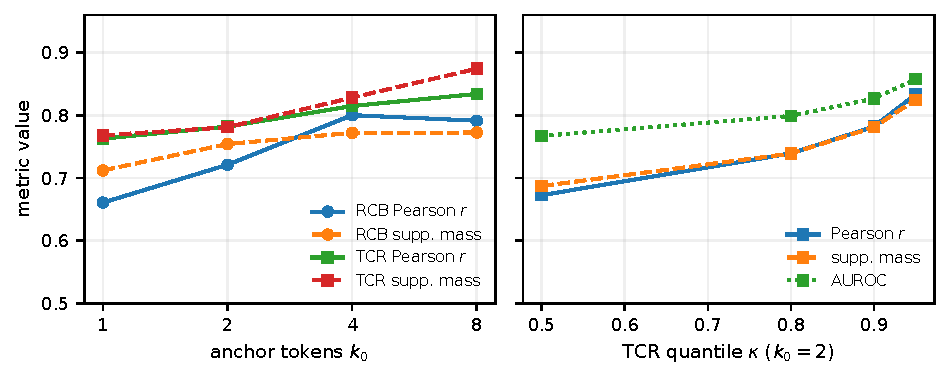
\includegraphics[width=0.85\linewidth]{figures/fig_gatt_sensitivity.pdf}
\caption{Sensitivity of GATT ($v_{\text{logvol}}$, floor-shifted link, $200$ instances). Left: anchor tokens $k_0$ for RCB and TCR ($\kappa = 0.9$). Right: background quantile $\kappa$ for TCR ($k_0 = 2$).}
\label{fig:exp_sensitivity}
\end{figure}

\paragraph{VATT: basis size.}
VATT is insensitive to the number of directions per snippet. With $v_{\text{proj}}$ and $k \in \{1, 2, 4, 8, 16\}$, Pearson $r$ stays at $0.91$, AUROC at $0.92$--$0.93$, MAE at $5.7$--$5.9$\,pp and P@2 at $86.8$--$88.8\%$ (best at $k = 2$). The reason is that the read-outs concentrate on the dominant value directions of the few attended anchor tokens: bases that retain $40\%$, $65\%$, $77\%$ and $87\%$ of the attention-weighted value energy ($k = 1, 4, 8, 16$) already explain $80\%$, $97\%$, $99\%$ and $99.9\%$ of the read-out energy. One pooled read-out vector per snippet (VATT-pool, Section~\ref{subsec:vatt}) is slightly worse with $v_{\text{logvol}}$ ($r = 0.89$, AUROC $0.90$ vs.\ $0.90$ and $0.92$), consistent with Proposition~\ref{prop:set_values}(v).

\begin{table}[t]
\centering
\small
\setlength{\tabcolsep}{3.5pt}
\begin{tabular}{llcccccccccc}
\toprule
 & & \multicolumn{10}{c}{Global layers $g$ ($\ell = 6g - 1$)} \\
\cmidrule(lr){3-12}
$v$ & Layers & 1 & 2 & 3 & 4 & 5 & 6 & 7 & 8 & 9 & 10 \\
\midrule
$v_{\mathrm{proj}}$ & first $g$ & 0.76 & 0.81 & 0.84 & 0.88 & 0.91 & 0.92 & 0.92 & 0.92 & 0.92 & \textbf{0.93} \\
$v_{\mathrm{proj}}$ & only $g$ & 0.76 & 0.84 & 0.87 & 0.91 & \textbf{0.93} & 0.92 & 0.92 & 0.90 & \textbf{0.93} & \textbf{0.93} \\
$v_{\mathrm{logvol}}$ & first $g$ & 0.59 & 0.64 & 0.71 & 0.80 & 0.85 & 0.89 & 0.91 & 0.91 & \textbf{0.92} & 0.91 \\
$v_{\mathrm{logvol}}$ & only $g$ & 0.59 & 0.68 & 0.80 & 0.90 & \textbf{0.95} & 0.93 & 0.94 & 0.89 & 0.93 & 0.90 \\
\bottomrule
\end{tabular}
\caption{Supporting-fact AUROC of VATT ($k = k_r = 8$, floor-shifted link, $200$ instances) when restricting the heads to the first $g$ global layers or to the $g$-th global layer only.}
\label{tab:vatt_layers}
\end{table}

\paragraph{VATT: how many global layers are needed?}
Table~\ref{tab:vatt_layers} restricts VATT to the first $g$ global layers or to a single one. With $v_{\text{proj}}$, the first five global layers ($\ell \le 29$) reach AUROC $0.91$ and P@2 $85.5\%$, the first seven reach AUROC $0.92$ and P@2 $88.0\%$, and the remaining layers add at most $0.01$ AUROC, so extracting values from half of the global layers suffices. The first global layer alone is weak (AUROC $0.76$), and single-layer accuracy peaks in the middle of the network: the fifth global layer ($\ell = 29$) reaches AUROC $0.93$ with $v_{\text{proj}}$ and $0.95$ with $v_{\text{logvol}}$ (P@2 $90.5\%$). Because $v_{\text{logvol}}$ sums per-head mutual informations, it is more sensitive than the energy-weighted $v_{\text{proj}}$ to uninformative early heads (AUROC $0.59$ with the first global layer). The same depth profile appears for the direct attention heuristics (Section~\ref{subsec:exp_citation_easton}).

\subsection{Monte Carlo Error and Cost}
\label{subsec:exp_cost}

\paragraph{Permutation sampling.}
Enumerating all $2^n$ coalitions of the Gram matrix gives the exact Monte Carlo error of the $K$-permutation estimator (Figure~\ref{fig:exp_mc}). The median relative error $\|\bar{\mathbf{m}}_K - \boldsymbol{\Phi}\|_\infty / \|\boldsymbol{\Phi}\|_1$ decays as $K^{-1/2}$, as predicted by Theorem~\ref{thm:bernstein_shapley}. At $K = 100$, it is $1.1\%$ (RCB), $1.4\%$ (EATT) and $2.4\%$ (TCR) for $v_{\text{logvol}}$ (below $0.8\%$ for all three at $K = 1000$), compared with $4.1$--$8.9\%$ for $v_{\text{ent}}$ and up to $30.5\%$ for $v_{\text{vol}}$ on TCR, reflecting the non-negative bounded marginal gains in~\eqref{eq:marginal_logvol}.

\begin{figure}[t]
\centering
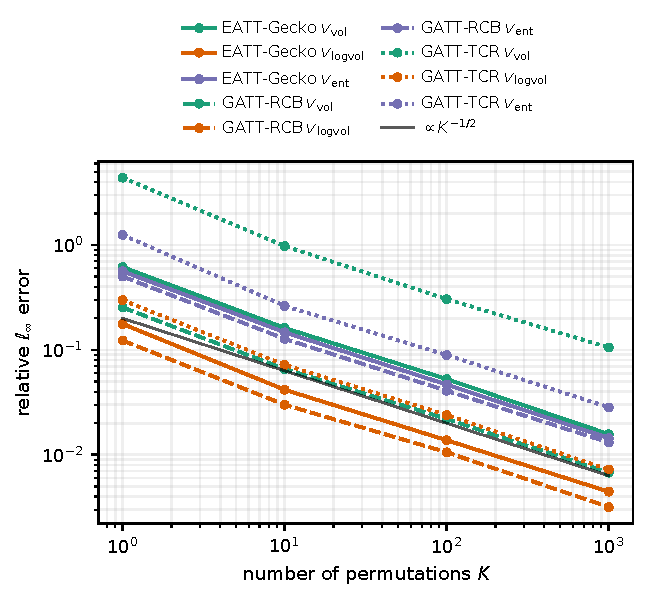
\includegraphics[width=0.58\linewidth]{figures/fig_mc_convergence.pdf}
\caption{Median relative $\ell_\infty$ error of the $K$-permutation Shapley estimator with respect to exact $2^n$ enumeration on the Gram matrix ($n = 6$, $200$ instances). Line style: Gram matrix; color: value function.}
\label{fig:exp_mc}
\end{figure}

\paragraph{Wall-clock cost.}
On $8$ TPU v6e chips, exact $2^n$ likelihood Shapley takes $8.3$\,s per instance ($63.7$ forward passes), $10$-permutation LLH-Shapley $5.7$\,s ($34.9$ distinct passes), and $16$-step Integrated Gradients $8.0$\,s. GATT needs one forward pass on $(p, S, r)$ to extract the global-layer queries, keys and logits ($1.0$\,s), $1.1$\,s to assemble both Gram matrices, and $15$\,ms of CPU time for $K = 100$ permutations across all three value functions. VATT needs one forward pass to extract attention rows and value vectors ($0.94$\,s), $0.48$\,s on the accelerator for the per-head bases and Gram blocks, and about $0.24$\,s of CPU time to tabulate all $64$ coalitions for one configuration; exact Shapley values then take less than $1$\,ms. Including the empty-context pass for $w$, both use two LLM forward passes, independently of $n$ and $K$. EATT needs $n + 1$ encoder calls and $30$\,ms of CPU time and touches the LLM only for $w$.

\paragraph{Answer-correct instances.}
Restricting the evaluation to the $160$ instances with a correct answer leaves every conclusion unchanged within confidence intervals (Appendix~\ref{app:exp_correct}). For example, VATT with $v_{\text{proj}}$ reaches $r = 0.91$, $\rho = 0.79$, MAE $5.8$\,pp, AUROC $0.93$ and P@2 $88.4\%$, and with $v_{\text{vol}}$ (rectified) $\rho = 0.86$, $\tau = 0.81$.


\subsection{Discussion and Limitations}
\label{subsec:exp_discussion}

Even exact likelihood Shapley values inherit the positional sensitivity of causal LLM prompting~\cite{liu2024lost}, so agreement with $v_{\text{LL}}$ complements rather than replaces the supporting-fact evaluation; conversely, supporting-fact labels strictly apply only when the model answers correctly, which is why we repeat all results on the answer-correct instances. All three geometric families explain the observed computation of a single forward pass rather than the counterfactual effect of removing a snippet, which $v_{\text{LL}}$ measures. For VATT, the value vector of a context token is computed from a residual stream that already mixes information from earlier tokens, including other snippets, and information that reaches the response through local attention layers is ignored (Remark~\ref{rem:vatt_limitations}). For $n = 20$, the reference is a $128$-mask ContextCite surrogate, which favors the ContextCite baseline in the agreement metrics; we therefore rely on the supporting-fact labels for MuSiQue and on the label-free LDS and top-$k$ drops for CNN/DailyMail. Our benchmarks stop at $n = 20$ snippets. With a fixed budget, the ablation surrogates already degrade between $n = 6$ and $n = 20$ (KernelSHAP from $r = 0.91$ to $0.61$), while the geometric methods need two passes for any $n$; long-context RAG with hundreds of retrieved chunks, where even a high-budget reference is unavailable, is the natural next test, as are the error-weighted GATT variants of Remark~\ref{rem:error_weighted}.

%%%%%%%%%%%%%%%%%%%%%%%%%%%%%%%%%%%%%%%%%%%%%%%%%%%%%%%%%%%%%%%%%%%%%%%%%%%%%%%%%%%%%%%%%%%%%%%%%%%%%%%%%%%%
\section{Conclusions}
\label{sec:conclusions}

We formulated context attribution for LLMs as a cooperative game whose value functions are defined by the geometry of the snippets and the response rather than by the likelihood of the response under ablated contexts. The three value functions---volume difference, log-volume and spectral entropy---depend only on a Gram matrix, so the same Shapley machinery, link functions and Monte Carlo guarantees apply whatever produces the Gram matrix. The log-volume is the mutual information of a Gaussian channel and coincides with the likelihood game under a power-law likelihood condition, which connects the geometric games to the likelihood-based attribution of~\cite{nematov2025source}. We instantiated the framework with three sources of geometry: an external text encoder (EATT), the query--key routing of the LLM (GATT), and the value subspaces from which the response reads (VATT), for which we extended the value functions from single vectors to sets of vectors via principal angles.

On $200$ HotpotQA instances with Gemma~4 31B and exact $2^n$ likelihood Shapley values as reference, all three families attribute with two LLM passes, independently of the number of snippets. The source of the geometry matters most. EATT and GATT agree with the reference at Pearson $r = 0.72$--$0.78$; VATT, which uses the representations through which the snippets actually influence the response, reaches $r = 0.91$, halves the error to $5.8$ percentage points, matches KernelSHAP with $23$ LLM passes, and exceeds every ablation baseline and the exact reference itself in supporting-fact AUROC ($0.93$). The same conclusions hold on 2WikiMultihopQA ($n = 10$, exact reference), MuSiQue ($n = 20$) and CNN/DailyMail summarization: VATT reaches $r = 0.88$--$0.94$ with two passes, recovers the supporting facts as well as or better than every ablation baseline (AUROC $0.99$ on 2WikiMultihopQA and $0.93$ on MuSiQue), and overtakes fixed-budget KernelSHAP as $n$ grows. With duplicated or paraphrased evidence, the Shapley-based attributions split the credit between the copies, whereas leave-one-out assigns them almost nothing in $35$--$51\%$ of the instances. The log-volume is the robust default across geometries, the volume difference gives the best rankings when every player has an orthonormal basis (Spearman $0.84$ for VATT), and, because components shared by all snippets produce a common offset, the floor-shifted link is needed by every geometric game except the volume difference on VATT, whose redundancy penalty already assigns non-positive credit to the overlapping distractors. Gradient-based attribution of the same likelihood fails because of saturation and off-manifold interpolation, and the first half to two-thirds of the global layers suffice for the attention-based methods.

In practice, we recommend VATT with a few directions per snippet, the mid-network global layers and the floor-shifted link when the generation pass of the model is available---with the projected read-out energy for a handful of snippets and the log-volume when many snippets contribute ($n \ge 20$ or summarization)--- and EATT with the log-volume when only black-box access to the model is possible. Subset-ablation methods remain more accurate when $25$ or more LLM passes per instance are affordable ($r \ge 0.97$). The main open directions are long-context retrieval with hundreds of chunks, where linear-cost ablation becomes prohibitive and even high-budget references are unavailable, and combining the routing (QK) and content (OV) views of attention in a single game.

%%%%%%%%%%%%%%%%%%%%%%%%%%%%%%%%%%%%%%%%%%%%%%%%%%%%%%%%%%%%%%%%%%%%%%%%%%%%%%%%%%%%%%%%%%%%%%%%%%%%%%%%%%
%%%%%%%%%%%%%%%%%%%%%%%%%%%%%%%%%%%%%%%%%%%%%%%%%%%%%%%%%%%%%%%%%%%%%%%%%%%%%%%%%%%%%%%%%%%%%%%%%%%%%%%%%%



\bibliographystyle{alpha}
\bibliography{sample}


%%%%%%%%%%%%%%%%%%%%%%%%%%%%%%%%%%%%%%%%%%%%%%%%%%%%%%%%%%%%%%%%%%%%%%%%%%%%%%%%%%%%%%%%%%%%%%%%%%%%%%%%%%
\newpage
\appendix 

\section{Properties of Embedding based Value Functions}
\label{app:prop_emb}

\begin{proposition}\label{prop:v_logvol}
The log-volume value function $v_{\text{logvol}}$ satisfies the following properties:
\begin{enumerate}
    \item \textbf{Monotonicity and Non-Negativity:} $v_{\text{logvol}}(S') \ge 0$ for all $S' \subseteq [n]$, and $v_{\text{logvol}}$ is strictly monotone: $S' \subseteq T' \implies v_{\text{logvol}}(S') \le v_{\text{logvol}}(T')$.
    \item \textbf{Exact Marginal Gain:} For any $i \notin S'$, let $\mathbf{r}_{\perp} := (\mathbf{I}_d - \mathbf{P}_{\{S'\}})\mathbf{r}$ and $\mathbf{m}_{i, \perp} := (\mathbf{I}_d - \mathbf{P}_{\{S'\}})\mathbf{m}_i$ be the residual vectors orthogonal to $\mathcal{U}_{\{S'\}}$. If $\mathbf{m}_{i, \perp} \neq \mathbf{0}$, the marginal gain evaluates in closed form to:
    \begin{align}\label{eq:marginal_logvol}
        \Delta v_{\text{logvol}}(S', i) = -\frac{1}{2} \log\big(1 - \cos^2 \theta_i(S')\big) \ge 0, \qquad \text{where } \cos \theta_i(S') := \frac{\langle \mathbf{r}_{\perp}, \mathbf{m}_{i, \perp} \rangle}{\|\mathbf{r}_{\perp}\|_2 \|\mathbf{m}_{i, \perp}\|_2},
    \end{align}
    and $\Delta v_{\text{logvol}}(S', i) := 0$ if $\mathbf{m}_{i, \perp} = \mathbf{0}$.
    \item \textbf{Guaranteed Non-Negative Shapley Allocations:} Every snippet receives a non-negative raw Shapley value: $\phi_i(v_{\text{logvol}}) \ge 0$ for all $i \in [n]$, with $\sum_{i=1}^n \phi_i(v_{\text{logvol}}) = -\log d_{\perp}(\mathbf{r}, \mathcal{U}_{\{[n]\}})$.
\end{enumerate}
\end{proposition}

\begin{proof}
(1) Because $\|\mathbf{r}\|_2 = 1$, the orthogonal distance satisfies $d_{\perp}(\mathbf{r}, \mathcal{U}_{\{S'\}}) \in [0, 1]$, which implies $-\log d_{\perp} \ge 0$. Adding vectors expands the subspace ($\mathcal{U}_{\{S'\}} \subseteq \mathcal{U}_{\{T'\}}$), which monotonically non-increases the residual distance, rendering $v_{\text{logvol}}$ monotone. 
(2) Since $\mathcal{U}_{\{S' \cup \{i\}\}} = \mathcal{U}_{\{S'\}} \oplus \operatorname{span}(\mathbf{m}_{i, \perp})$, projecting $\mathbf{r}_{\perp}$ onto the unit vector $\mathbf{u} = \mathbf{m}_{i, \perp} / \|\mathbf{m}_{i, \perp}\|_2$ yields:
\begin{align*}
    d_{\perp}^2(\mathbf{r}, \mathcal{U}_{\{S' \cup \{i\}\}}) = \|\mathbf{r}_{\perp}\|_2^2 - \langle \mathbf{r}_{\perp}, \mathbf{u} \rangle^2 = \|\mathbf{r}_{\perp}\|_2^2 \big(1 - \cos^2 \theta_i(S')\big).
\end{align*}
Taking $-\frac{1}{2}\log$ of the ratio $d_{\perp}^2(\mathbf{r}, \mathcal{U}_{\{S' \cup \{i\}\}}) / d_{\perp}^2(\mathbf{r}, \mathcal{U}_{\{S'\}})$ yields Equation~\eqref{eq:marginal_logvol}. By the Cauchy--Schwarz inequality, $\cos^2 \theta_i(S') \in [0, 1]$, ensuring the argument of the logarithm is in $(0, 1]$, so $\Delta v_{\text{logvol}} \ge 0$. 
(3) Follows directly because the Shapley value is a convex combination of non-negative marginal gains.
\end{proof}


\begin{proposition}[Spectral Mutual Information Interpretation]\label{prop:v_ent}
Let $\boldsymbol{\rho} := \boldsymbol{\rho}(\mathbf{G}^{+}_{\{S'\}})$ and $\boldsymbol{\sigma} := \boldsymbol{\rho}(\bar{\mathbf{G}}^{+}_{\{S'\}})$. Then:
\begin{enumerate}
    \item $v_{\text{ent}}(S') = D(\boldsymbol{\rho} \,\|\, \boldsymbol{\sigma}) := \operatorname{Tr}\big(\boldsymbol{\rho}(\log \boldsymbol{\rho} - \log \boldsymbol{\sigma})\big)$, where $D(\cdot \,\|\, \cdot)$ is the quantum relative entropy.
    \item $v_{\text{ent}}(S') \ge 0$, with $v_{\text{ent}}(S') = 0$ if and only if $\mathbf{M}_{\{S'\}}^\top \mathbf{r} = \mathbf{0}$ ($\mathbf{r} \perp \mathcal{U}_{\{S'\}}$).
    \item $v_{\text{ent}}(S') \le \log 2$ for all coalitions, ensuring $v_{\text{ent}}$ is universally bounded without regularization.
\end{enumerate}
\end{proposition}

\begin{proof}
(1) Since $\boldsymbol{\sigma}$ is block-diagonal, $\log \boldsymbol{\sigma}$ is also block-diagonal on its support. Because the diagonal blocks of $\boldsymbol{\rho}$ and $\boldsymbol{\sigma}$ are identical, $\operatorname{Tr}(\boldsymbol{\rho} \log \boldsymbol{\sigma}) = \operatorname{Tr}(\boldsymbol{\sigma} \log \boldsymbol{\sigma}) = -\mathcal{H}(\bar{\mathbf{G}}^{+}_{\{S'\}})$, establishing $v_{\text{ent}}(S') = D(\boldsymbol{\rho} \,\|\, \boldsymbol{\sigma})$. 
(2) By Klein's inequality, $D(\boldsymbol{\rho} \,\|\, \boldsymbol{\sigma}) \ge 0$, with equality holding if and only if $\boldsymbol{\rho} = \boldsymbol{\sigma}$, which occurs precisely when the cross-term $\mathbf{g}_{\{S'\}} = \mathbf{M}_{\{S'\}}^\top \mathbf{r} = \mathbf{0}$. 
(3) Noting that $\boldsymbol{\sigma} = \frac{1}{2}(\boldsymbol{\rho} + \mathbf{U}\boldsymbol{\rho}\mathbf{U}^\top)$ for the unitary matrix $\mathbf{U} = \operatorname{diag}(\mathbf{I}_k, -1)$, subadditivity of entropy bounds the entropy increase by $\mathcal{H}(\boldsymbol{\sigma}) - \mathcal{H}(\boldsymbol{\rho}) \le \log 2$.
\end{proof}

\section{Tractable Approximation of Shapley value via Permutation Sampling}
\label{subsec:tractable_approximation}

To overcome the exponential $\mathcal{O}(2^n)$ bottleneck of the exact Shapley formulation, one can approximate the attribution vector using Monte Carlo sampling over permutations. This approach is widely considered part of the literature's folklore. The permutation-based Monte Carlo approximation of the Shapley value was first introduced in cooperative game theory by Mann and Shapley~\cite{mann1960values}.  We formalize this unbiased estimator and provide its proof below.

\begin{lemma}\label{lemma:unbiased_estimator}
\textbf{(Unbiased Estimator of the Shapley Vector).}
Let $\boldsymbol{\Phi}(v) = (\phi_1(v), \dots, \phi_n(v))^\top \in \mathbb{R}^n$ be the exact Shapley attribution vector under any valid characteristic function $v$ with $v(\emptyset) = 0$. Let $\Pi([n])$ denote the symmetric group of all $n!$ permutations of the index set $[n]$. For a permutation $\pi \in \Pi([n])$ sampled uniformly at random, let $S_i^\pi := \{j \in [n] \mid \pi(j) < \pi(i)\}$ denote the subset of players preceding player $i$ in $\pi$. Define the stochastic marginal gain vector $\mathbf{m}^\pi := (m_1^\pi, \dots, m_n^\pi)^\top \in \mathbb{R}^n$ where $m_i^\pi := \Delta v(S_i^\pi, i)$. Then $\mathbf{m}^\pi$ is an unbiased estimator of the true Shapley vector:
\begin{align}
    \mathbb{E}_{\pi \sim \Pi([n])}[\mathbf{m}^\pi] = \boldsymbol{\Phi}(v).
\end{align}
\end{lemma}

By generating a small set of $K \ll n!$ uniform random permutations, the true Shapley vector can be approximated in strictly polynomial time $\mathcal{O}(K \cdot n \cdot \mathcal{C})$, where $\mathcal{C}$ is the evaluation cost of the characteristic function.  While evaluating even a small number of paths is prohibitively expensive when using autoregressive forward passes ($C = \mathcal{C}_{\text{LLM}}$), this approximation becomes extremely practical under our proposed embedding-based geometric frameworks where $\mathcal{C} = \mathcal{O}(d^2)$, see in Section \ref{}.


\begin{proofof}{Lemma~\ref{lemma:unbiased_estimator}}
To show that the expectation holds, we evaluate the expectation of an arbitrary $i$-th component, $\mathbb{E}_\pi[m_i^\pi]$. Since the permutation $\pi$ is sampled uniformly from $\Pi([n])$, each permutation occurs with probability $1/n!$. The expected value of the marginal gain of snippet $i$ is:
\begin{align}
    \mathbb{E}_{\pi}[m_i^\pi] = \sum_{\pi \in \Pi([n])} \frac{1}{n!} \Delta v(S_i^\pi, i).
\end{align}
We partition the summation over all permutations by grouping them according to the unique unordered subset of preceding elements. For a fixed subset $S' \subseteq [n] \setminus \{i\}$ of size $k = |S'|$, we count the number of permutations $\pi \in \Pi([n])$ that satisfy $S_i^\pi = S'$. For snippet $i$ to be preceded by precisely the elements in $S'$:
\begin{enumerate}
    \item The $k$ elements within $S'$ can be arranged in the first $k$ positions of the permutation in $k!$ different ways.
    \item The element $i$ must be fixed at position $k + 1$.
    \item The remaining $(n - k - 1)$ elements in $[n] \setminus (S' \cup \{i\})$ can be arranged in the remaining positions in $(n - k - 1)!$ different ways.
\end{enumerate}
Thus, there are exactly $|S'|!(n - |S'| - 1)!$ permutations that yield the exact marginal context subset $S_i^\pi = S'$. Replacing the sum over permutations with a sum over all possible subsets $S' \subseteq [n] \setminus \{i\}$ weighted by this combinatorial factor yields:
\begin{align}
    \mathbb{E}_{\pi}[m_i^\pi] = \sum_{S' \subseteq [n] \setminus \{i\}} \frac{|S'|!(n - |S'| - 1)!}{n!} \Delta v(S', i).
\end{align}
This formulation is exactly the canonical subset-based definition of the exact Shapley value $\phi_i(v)$. Since $\mathbb{E}_{\pi}[m_i^\pi] = \phi_i(v)$ holds for every element $i \in [n]$, it follows that the joint vector expectation exactly recovers the full attribution vector $\mathbb{E}_\pi[\mathbf{m}^\pi] = \boldsymbol{\Phi}(v)$, completing the proof.
\end{proofof}

%%%%%%%%%%%%%%%%%%%%%%%%%%%%%%%%%%%%%%%%%%%%%%%%%%%%%%%%%%%%%%%%%%%%%%%%%%%%%%%%%%%%%%%%%%%%%%%%%%%%%%%%%%%%

\section{Covariance Structure and Bernstein Concentration}
\label{app:bernstein_concentration}

Let $\pi_1, \dots, \pi_K \overset{\text{i.i.d.}}{\sim} \Pi([n])$ be $K$ permutations sampled uniformly at random. For each trajectory $\pi_k$, the stochastic marginal gain vector is $\mathbf{m}^{\pi_k} = (m_1^{\pi_k}, \dots, m_n^{\pi_k})^\top \in \mathbb{R}^n$, where $m_i^{\pi_k} := \Delta v(S_i^{\pi_k}, i)$. The empirical Monte Carlo Shapley estimator is:
\begin{align}
    \bar{\mathbf{m}}_K := \frac{1}{K} \sum_{k=1}^K \mathbf{m}^{\pi_k}, \qquad \text{with } \mathbb{E}[\bar{\mathbf{m}}_K] = \boldsymbol{\Phi}(v).
\end{align}

\paragraph{Telescoping Sum and Covariance Identity.}
Along any permutation $\pi$, the marginal contributions telescope across the entire grand coalition:
\begin{align}\label{eq:telescoping_sum}
    \sum_{i=1}^n m_i^\pi = \sum_{k=1}^n \Big( v(\{\pi_1, \dots, \pi_k\}) - v(\{\pi_1, \dots, \pi_{k-1}\}) \Big) = v([n]) - v(\emptyset) = v([n]).
\end{align}
Because the sum is a deterministic constant, $\operatorname{Var}\big(\sum_{i=1}^n m_i^\pi\big) = 0$. Expanding the variance of the sum yields the zero-sum cross-covariance identity:
\begin{align}\label{eq:zero_sum_cov}
    \sum_{j=1}^n \operatorname{Cov}(m_i^\pi, m_j^\pi) = 0 \quad \Longleftrightarrow \quad \sum_{j \neq i} \operatorname{Cov}(m_i^\pi, m_j^\pi) = -\sigma_i^2,
\end{align}
where $\sigma_i^2 := \operatorname{Var}(m_i^\pi) = \mathbb{E}[(m_i^\pi - \phi_i(v))^2]$. The negative total covariance demonstrates that individual coordinates compete directly for semantic volume along any single trajectory.

\paragraph{Bernstein Concentration Bound.}
Assume that the marginal contributions are bounded such that $\sup_{S', i} |\Delta v(S', i)| \le B$. Then for each player $i \in [n]$, the centered variable $X_k := m_i^{\pi_k} - \phi_i(v)$ satisfies $\mathbb{E}[X_k] = 0$, $\mathbb{E}[X_k^2] = \sigma_i^2$, and $|X_k| \le 2B$ almost surely.

\begin{theorem}\label{thm:bernstein_shapley}
Let $\sigma_{\max}^2 := \max_{i \in [n]} \sigma_i^2$. For any error tolerance $\epsilon > 0$, the empirical estimator $\bar{\mathbf{m}}_K$ concentrates around the exact Shapley vector $\boldsymbol{\Phi}(v)$ as:
\begin{align}
    \mathbb{P}\Big( \|\bar{\mathbf{m}}_K - \boldsymbol{\Phi}(v)\|_\infty \ge \epsilon \Big) \le 2n \exp\left( -\frac{K \epsilon^2}{2 \sigma_{\max}^2 + \frac{4}{3} B \epsilon} \right).
\end{align}
Consequently, to guarantee that $\|\bar{\mathbf{m}}_K - \boldsymbol{\Phi}(v)\|_\infty \le \epsilon$ with probability at least $1 - \delta$, it suffices to sample:
\begin{align}
    K \ge \left( \frac{2 \sigma_{\max}^2}{\epsilon^2} + \frac{4 B}{3 \epsilon} \right) \log\left( \frac{2n}{\delta} \right) = \mathcal{O}\left( \frac{\sigma_{\max}^2}{\epsilon^2} \log\left(\frac{n}{\delta}\right) \right)
\end{align}
permutations.
\end{theorem}

\begin{proof}
Applying Bernstein's inequality to the sum of $K$ independent, zero-mean, bounded random variables $\sum_{k=1}^K (m_i^{\pi_k} - \phi_i(v))$ yields:
\begin{align}
    \mathbb{P}\Big( |\bar{m}_{K, i} - \phi_i(v)| \ge \epsilon \Big) = \mathbb{P}\left( \left|\sum_{k=1}^K X_k\right| \ge K \epsilon \right) \le 2 \exp\left( -\frac{K^2 \epsilon^2}{2 K \sigma_i^2 + \frac{2}{3}(2B)(K \epsilon)} \right) = 2 \exp\left( -\frac{K \epsilon^2}{2 \sigma_i^2 + \frac{4}{3} B \epsilon} \right).
\end{align}
Applying the union bound over all $n$ coordinates immediately gives the $\ell_\infty$ bound. Setting the error probability equal to $\delta$ and solving for $K$ yields the sample complexity bound.
\end{proof}



%%%%%%%%%%%%%%%%%%%%%%%%%%%%%%%%%%%%%%%%%%%%%%%%%%%%%%%%%%%%%%%%%%%%%%%%%%%%%%%%%%%%%%%%%%%%%%%%%%%%%%%%%%%%
% Appendix material (place after \appendix).
%%%%%%%%%%%%%%%%%%%%%%%%%%%%%%%%%%%%%%%%%%%%%%%%%%%%%%%%%%%%%%%%%%%%%%%%%%%%%%%%%%%%%%%%%%%%%%%%%%%%%%%%%%%%
\section{Additional Experimental Results}
\label{app:exp_correct}

The supporting-fact labels of HotpotQA describe the evidence for the \emph{correct} answer. Table~\ref{tab:exp_correct} repeats Tables~\ref{tab:exp_main} and~\ref{tab:exp_values} on the $160$ instances ($80\%$) in which the generated response contains the normalized gold answer. All differences lie well within the confidence intervals. The exact likelihood reference places $95.7\%$ of the credit on the supporting facts (AUROC $0.92$, P@2 $86.6\%$); EATT with $v_{\text{logvol}}$ reaches $92.8\%$ mass and AUROC $0.91$; GATT-TCR with $v_{\text{logvol}}$ reaches $r = 0.79$ and $79.9\%$ mass; VATT with $v_{\text{proj}}$ reaches $r = 0.91$, $92.4\%$ mass, AUROC $0.93$ and P@2 $88.4\%$; and the mean global context weight remains $w = 0.95$.

\begin{table}[t]
\centering
\small
\setlength{\tabcolsep}{2.6pt}
\resizebox{\linewidth}{!}{%
\begin{tabular}{lllcccccccccc}
\toprule
 & & & & \multicolumn{5}{c}{Agreement with Exact LLH-Shapley} & \multicolumn{3}{c}{Supporting facts} \\
\cmidrule(lr){5-9} \cmidrule(lr){10-12}
Method & $v$ & Link & Passes & Pearson $r$ & Spearman $\rho$ & Kendall $\tau$ & MAE (pp) $\downarrow$ & Top-1 (\%) & Mass (\%) & AUROC & P@2 (\%) \\
\midrule
\multicolumn{12}{l}{\emph{Proposed geometric methods (two LLM passes)}} \\
EATT (Gecko) & $v_{\mathrm{vol}}$ & floor & $2^\dagger$ & 0.73{\scriptsize$\pm$0.06} & 0.62{\scriptsize$\pm$0.05} & 0.54{\scriptsize$\pm$0.04} & 10.9{\scriptsize$\pm$1.3} & 69.4{\scriptsize$\pm$7.2} & 89.5{\scriptsize$\pm$2.5} & 0.88{\scriptsize$\pm$0.03} & 78.4{\scriptsize$\pm$3.8} \\
EATT (Gecko) & $v_{\mathrm{logvol}}$ & floor & $2^\dagger$ & 0.74{\scriptsize$\pm$0.05} & 0.69{\scriptsize$\pm$0.04} & 0.60{\scriptsize$\pm$0.03} & 10.7{\scriptsize$\pm$1.4} & 69.4{\scriptsize$\pm$7.2} & \textbf{92.8}{\scriptsize$\pm$2.1} & 0.91{\scriptsize$\pm$0.02} & 84.1{\scriptsize$\pm$3.6} \\
EATT (Gecko) & $v_{\mathrm{ent}}$ & floor & $2^\dagger$ & 0.73{\scriptsize$\pm$0.05} & 0.66{\scriptsize$\pm$0.04} & 0.58{\scriptsize$\pm$0.04} & 11.0{\scriptsize$\pm$1.3} & 65.6{\scriptsize$\pm$7.5} & 86.7{\scriptsize$\pm$2.6} & 0.89{\scriptsize$\pm$0.03} & 79.7{\scriptsize$\pm$3.8} \\
\addlinespace[2pt]
GATT-RCB & $v_{\mathrm{vol}}$ & floor & 2.0 & 0.70{\scriptsize$\pm$0.06} & 0.58{\scriptsize$\pm$0.05} & 0.50{\scriptsize$\pm$0.05} & 12.5{\scriptsize$\pm$1.6} & 64.4{\scriptsize$\pm$7.5} & 74.5{\scriptsize$\pm$3.4} & 0.82{\scriptsize$\pm$0.03} & 70.6{\scriptsize$\pm$4.7} \\
GATT-RCB & $v_{\mathrm{logvol}}$ & floor & 2.0 & 0.72{\scriptsize$\pm$0.06} & 0.61{\scriptsize$\pm$0.05} & 0.53{\scriptsize$\pm$0.04} & 11.9{\scriptsize$\pm$1.5} & 66.2{\scriptsize$\pm$7.5} & 76.1{\scriptsize$\pm$3.3} & 0.83{\scriptsize$\pm$0.03} & 72.5{\scriptsize$\pm$4.4} \\
GATT-RCB & $v_{\mathrm{ent}}$ & floor & 2.0 & 0.74{\scriptsize$\pm$0.05} & 0.62{\scriptsize$\pm$0.04} & 0.54{\scriptsize$\pm$0.04} & 12.0{\scriptsize$\pm$1.5} & 66.9{\scriptsize$\pm$7.2} & 73.3{\scriptsize$\pm$3.3} & 0.84{\scriptsize$\pm$0.03} & 71.2{\scriptsize$\pm$4.4} \\
\addlinespace[2pt]
GATT-TCR & $v_{\mathrm{vol}}$ & floor & 2.0 & 0.28{\scriptsize$\pm$0.07} & 0.35{\scriptsize$\pm$0.05} & 0.30{\scriptsize$\pm$0.04} & 20.5{\scriptsize$\pm$1.5} & 23.8{\scriptsize$\pm$6.6} & 46.7{\scriptsize$\pm$4.3} & 0.68{\scriptsize$\pm$0.03} & 52.8{\scriptsize$\pm$3.4} \\
GATT-TCR & $v_{\mathrm{logvol}}$ & floor & 2.0 & 0.79{\scriptsize$\pm$0.05} & 0.64{\scriptsize$\pm$0.04} & 0.56{\scriptsize$\pm$0.04} & 10.0{\scriptsize$\pm$1.4} & 76.2{\scriptsize$\pm$6.6} & 79.9{\scriptsize$\pm$3.2} & 0.84{\scriptsize$\pm$0.03} & 70.6{\scriptsize$\pm$4.1} \\
GATT-TCR & $v_{\mathrm{ent}}$ & floor & 2.0 & 0.31{\scriptsize$\pm$0.07} & 0.36{\scriptsize$\pm$0.05} & 0.31{\scriptsize$\pm$0.04} & 20.2{\scriptsize$\pm$1.5} & 26.9{\scriptsize$\pm$6.6} & 46.2{\scriptsize$\pm$4.2} & 0.67{\scriptsize$\pm$0.03} & 51.2{\scriptsize$\pm$4.1} \\
\addlinespace[2pt]
VATT & $v_{\mathrm{proj}}$ & floor & 2.0 & \textbf{0.91}{\scriptsize$\pm$0.03} & 0.79{\scriptsize$\pm$0.02} & 0.70{\scriptsize$\pm$0.02} & \textbf{5.8}{\scriptsize$\pm$0.8} & \textbf{81.9}{\scriptsize$\pm$5.9} & 92.4{\scriptsize$\pm$2.1} & \textbf{0.93}{\scriptsize$\pm$0.02} & \textbf{88.4}{\scriptsize$\pm$3.3} \\
VATT & $v_{\mathrm{logvol}}$ & floor & 2.0 & 0.90{\scriptsize$\pm$0.03} & 0.77{\scriptsize$\pm$0.02} & 0.68{\scriptsize$\pm$0.02} & 6.3{\scriptsize$\pm$0.8} & 79.4{\scriptsize$\pm$6.2} & 90.3{\scriptsize$\pm$2.2} & 0.92{\scriptsize$\pm$0.02} & 85.9{\scriptsize$\pm$3.6} \\
VATT & $v_{\mathrm{vol}}$ & rect. & 2.0 & 0.89{\scriptsize$\pm$0.03} & \textbf{0.86}{\scriptsize$\pm$0.03} & \textbf{0.81}{\scriptsize$\pm$0.03} & 6.8{\scriptsize$\pm$0.9} & 77.5{\scriptsize$\pm$6.6} & 91.9{\scriptsize$\pm$2.6} & 0.92{\scriptsize$\pm$0.02} & 86.2{\scriptsize$\pm$3.6} \\
VATT & $v_{\mathrm{ent}}$ & floor & 2.0 & 0.89{\scriptsize$\pm$0.03} & 0.76{\scriptsize$\pm$0.02} & 0.67{\scriptsize$\pm$0.02} & 7.1{\scriptsize$\pm$0.8} & 78.1{\scriptsize$\pm$6.2} & 87.1{\scriptsize$\pm$2.4} & 0.91{\scriptsize$\pm$0.03} & 84.4{\scriptsize$\pm$3.7} \\
\midrule
\multicolumn{12}{l}{\emph{Gradient and subset-ablation baselines}} \\
Gradient $\times$ Input & $\nabla F$ & rect. & $2.0^\ddagger$ & 0.00{\scriptsize$\pm$0.07} & 0.02{\scriptsize$\pm$0.07} & 0.01{\scriptsize$\pm$0.06} & 25.8{\scriptsize$\pm$1.6} & 19.4{\scriptsize$\pm$6.2} & 31.8{\scriptsize$\pm$4.9} & 0.49{\scriptsize$\pm$0.04} & 30.6{\scriptsize$\pm$4.5} \\
Integrated Gradients (16) & $\nabla F$ & rect. & $17.0^\ddagger$ & 0.04{\scriptsize$\pm$0.07} & 0.08{\scriptsize$\pm$0.07} & 0.07{\scriptsize$\pm$0.06} & 24.6{\scriptsize$\pm$1.2} & 16.2{\scriptsize$\pm$5.6} & 36.0{\scriptsize$\pm$4.9} & 0.53{\scriptsize$\pm$0.04} & 34.7{\scriptsize$\pm$4.7} \\
LOO & $v_{\mathrm{LL}}$ & rect. & 8.0 & 0.97{\scriptsize$\pm$0.02} & 0.78{\scriptsize$\pm$0.03} & 0.72{\scriptsize$\pm$0.03} & 3.4{\scriptsize$\pm$0.6} & 95.0{\scriptsize$\pm$3.4} & 93.8{\scriptsize$\pm$2.7} & 0.92{\scriptsize$\pm$0.02} & 87.5{\scriptsize$\pm$3.8} \\
KernelSHAP (32) & $v_{\mathrm{LL}}$ & rect. & 23.3 & 0.90{\scriptsize$\pm$0.03} & 0.79{\scriptsize$\pm$0.03} & 0.74{\scriptsize$\pm$0.03} & 6.0{\scriptsize$\pm$0.8} & 81.9{\scriptsize$\pm$5.9} & 85.2{\scriptsize$\pm$2.6} & 0.87{\scriptsize$\pm$0.03} & 76.9{\scriptsize$\pm$4.1} \\
ContextCite (32) & $v_{\mathrm{LL}}$ & rect. & 25.1 & 0.99{\scriptsize$\pm$0.01} & 0.91{\scriptsize$\pm$0.02} & 0.87{\scriptsize$\pm$0.02} & 2.6{\scriptsize$\pm$0.4} & 93.1{\scriptsize$\pm$4.1} & 92.7{\scriptsize$\pm$2.3} & 0.92{\scriptsize$\pm$0.02} & 86.9{\scriptsize$\pm$3.6} \\
LLH-Perm ($K=10$) & $v_{\mathrm{LL}}$ & rect. & 34.9 & 0.97{\scriptsize$\pm$0.01} & 0.90{\scriptsize$\pm$0.02} & 0.86{\scriptsize$\pm$0.03} & 2.7{\scriptsize$\pm$0.4} & 86.2{\scriptsize$\pm$5.3} & 94.4{\scriptsize$\pm$2.4} & 0.90{\scriptsize$\pm$0.02} & 84.1{\scriptsize$\pm$3.9} \\
\midrule
Exact LLH-Shapley (ref.) & $v_{\mathrm{LL}}$ & rect. & 63.7 & 1 & 1 & 1 & 0 & 100 & 95.7 & 0.92 & 86.6 \\
Uniform & -- & -- & 0 & -- & -- & -- & 23.7 & 10.0 & 33.8 & 0.50 & 19.4 \\
\bottomrule
\end{tabular}%
}
\caption{As Tables~\ref{tab:exp_main} and~\ref{tab:exp_values}, restricted to the $160$ instances in which the generated response contains the gold answer. Best entry among the proposed methods is in bold.}
\label{tab:exp_correct}
\end{table}


\paragraph{Citation and Easton V2.1 on answer-correct instances.}
Table~\ref{tab:exp_citation_easton_correct} repeats the separate evaluation of Section~\ref{subsec:exp_citation_easton} on the $160$ answer-correct instances. Every pattern from Table~\ref{tab:exp_citation_easton}---including prefix saturation by $m = 5$--$7$ global layers and the single-layer peak at $\ell = 29$ (\texttt{single5})---holds within roughly one percentage point: on \texttt{mean10}, Citation ($K_{\text{in}} = 3$) reaches AUROC $0.92$ and P@2 $86.6\%$ (with $g^{\text{fl},2}$ cutting MAE from $13.2$ to $5.9$\,pp and lifting supporting-fact mass from $64.8\%$ to $91.7\%$, and \texttt{mean7} reaching $5.5$\,pp MAE and $93.9\%$ mass), while Easton V2.1 (\texttt{top-2}) reaches $r = 0.92$, $\rho = 0.79$, MAE $6.4$\,pp, and $89.0\%$ mass under simplex normalization ($6.0$\,pp MAE and $89.8\%$ mass at \texttt{mean7}; $95.5\%$ mass and $5.9$\,pp MAE under $g^{\text{fl},2}$).

\begin{table}[t]
\centering
\small
\setlength{\tabcolsep}{2.8pt}
\resizebox{\linewidth}{!}{%
\begin{tabular}{lllcccccccc}
\toprule
 & & & \multicolumn{5}{c}{Agreement with Exact LLH-Shapley} & \multicolumn{3}{c}{Supporting facts} \\
\cmidrule(lr){4-8} \cmidrule(lr){9-11}
Heuristic & Red. & Link & Pearson $r$ & Spearman $\rho$ & Kendall $\tau$ & MAE (pp) $\downarrow$ & Top-1 (\%) & Mass (\%) & AUROC & P@2 (\%) \\
\midrule
\multicolumn{11}{l}{\emph{Simplex normalization (rectified link, $s_i / \sum_j s_j$, all $10$ global layers)}} \\
Citation ($K_{\mathrm{in}}{=}3, K_{\mathrm{out}}{=}10$) & \texttt{mean10} & rect. & 0.91{\scriptsize$\pm$0.02} & 0.77{\scriptsize$\pm$0.02} & 0.68{\scriptsize$\pm$0.02} & 13.2{\scriptsize$\pm$0.7} & 80.0{\scriptsize$\pm$5.9} & 64.8{\scriptsize$\pm$1.7} & 0.92{\scriptsize$\pm$0.02} & 86.6{\scriptsize$\pm$3.6} \\
Citation ($K_{\mathrm{in}}{=}1, K_{\mathrm{out}}{=}10$) & \texttt{mean10} & rect. & 0.91{\scriptsize$\pm$0.02} & 0.77{\scriptsize$\pm$0.02} & 0.68{\scriptsize$\pm$0.02} & 13.2{\scriptsize$\pm$0.7} & 80.6{\scriptsize$\pm$5.9} & 64.7{\scriptsize$\pm$1.7} & 0.92{\scriptsize$\pm$0.02} & 86.9{\scriptsize$\pm$3.6} \\
Citation ($K_{\mathrm{in}}{=}3, K_{\mathrm{out}}{=}10$) & \texttt{max10} & rect. & 0.89{\scriptsize$\pm$0.02} & 0.76{\scriptsize$\pm$0.02} & 0.67{\scriptsize$\pm$0.02} & 15.8{\scriptsize$\pm$0.7} & 80.6{\scriptsize$\pm$5.6} & 57.8{\scriptsize$\pm$1.5} & 0.92{\scriptsize$\pm$0.03} & 85.9{\scriptsize$\pm$3.7} \\
Citation ($K_{\mathrm{in}}{=}3, K_{\mathrm{out}}{=}10$) & \texttt{max10+sp24} & rect. & 0.89{\scriptsize$\pm$0.02} & 0.77{\scriptsize$\pm$0.02} & 0.68{\scriptsize$\pm$0.02} & 11.9{\scriptsize$\pm$0.9} & 81.2{\scriptsize$\pm$5.6} & 70.7{\scriptsize$\pm$2.2} & 0.92{\scriptsize$\pm$0.02} & 85.9{\scriptsize$\pm$3.6} \\
Easton Raw (all tokens) & \texttt{mean10} & rect. & 0.86{\scriptsize$\pm$0.03} & 0.72{\scriptsize$\pm$0.02} & 0.63{\scriptsize$\pm$0.03} & 16.1{\scriptsize$\pm$0.7} & 79.4{\scriptsize$\pm$6.2} & 56.0{\scriptsize$\pm$1.5} & 0.88{\scriptsize$\pm$0.02} & 80.0{\scriptsize$\pm$3.8} \\
Easton V2.1 (all tokens) & \texttt{mean10} & rect. & 0.85{\scriptsize$\pm$0.03} & 0.73{\scriptsize$\pm$0.02} & 0.64{\scriptsize$\pm$0.02} & 16.3{\scriptsize$\pm$0.7} & 78.1{\scriptsize$\pm$6.2} & 55.5{\scriptsize$\pm$1.5} & 0.89{\scriptsize$\pm$0.03} & 81.2{\scriptsize$\pm$4.1} \\
Easton Raw (top-2) & \texttt{mean10} & rect. & \textbf{0.92}{\scriptsize$\pm$0.02} & 0.79{\scriptsize$\pm$0.02} & 0.71{\scriptsize$\pm$0.03} & 6.5{\scriptsize$\pm$0.8} & 80.0{\scriptsize$\pm$5.6} & 88.9{\scriptsize$\pm$2.3} & 0.92{\scriptsize$\pm$0.02} & 85.3{\scriptsize$\pm$3.9} \\
Easton V2.1 (top-2) & \texttt{mean10} & rect. & \textbf{0.92}{\scriptsize$\pm$0.02} & 0.79{\scriptsize$\pm$0.02} & 0.72{\scriptsize$\pm$0.03} & 6.4{\scriptsize$\pm$0.8} & 81.2{\scriptsize$\pm$5.6} & 89.0{\scriptsize$\pm$2.2} & 0.92{\scriptsize$\pm$0.02} & 85.9{\scriptsize$\pm$3.8} \\
Easton V2.1 (top-2) & \texttt{max10} & rect. & 0.90{\scriptsize$\pm$0.02} & 0.77{\scriptsize$\pm$0.02} & 0.70{\scriptsize$\pm$0.03} & 7.7{\scriptsize$\pm$0.9} & \textbf{81.9}{\scriptsize$\pm$5.6} & 84.1{\scriptsize$\pm$2.7} & 0.90{\scriptsize$\pm$0.03} & 82.2{\scriptsize$\pm$4.1} \\
Easton V2.1 (top-2) & \texttt{max10+sp6} & rect. & 0.89{\scriptsize$\pm$0.03} & \textbf{0.80}{\scriptsize$\pm$0.03} & \textbf{0.75}{\scriptsize$\pm$0.03} & 7.2{\scriptsize$\pm$1.0} & 81.2{\scriptsize$\pm$5.9} & 87.4{\scriptsize$\pm$3.0} & 0.89{\scriptsize$\pm$0.03} & 79.7{\scriptsize$\pm$4.2} \\
\midrule
\multicolumn{11}{l}{\emph{Floor-shifted power link ($g^{\mathrm{fl},2}$, all $10$ global layers)}} \\
Citation ($K_{\mathrm{in}}{=}3, K_{\mathrm{out}}{=}10$) & \texttt{mean10} & floor & 0.91{\scriptsize$\pm$0.02} & 0.77{\scriptsize$\pm$0.02} & 0.68{\scriptsize$\pm$0.02} & 5.9{\scriptsize$\pm$0.8} & 80.0{\scriptsize$\pm$5.9} & 91.7{\scriptsize$\pm$2.2} & 0.92{\scriptsize$\pm$0.02} & 86.6{\scriptsize$\pm$3.6} \\
Citation ($K_{\mathrm{in}}{=}1, K_{\mathrm{out}}{=}10$) & \texttt{mean10} & floor & 0.91{\scriptsize$\pm$0.03} & 0.77{\scriptsize$\pm$0.02} & 0.68{\scriptsize$\pm$0.02} & 6.1{\scriptsize$\pm$0.8} & 80.6{\scriptsize$\pm$5.9} & 91.2{\scriptsize$\pm$2.3} & 0.92{\scriptsize$\pm$0.02} & 86.9{\scriptsize$\pm$3.6} \\
Citation ($K_{\mathrm{in}}{=}3, K_{\mathrm{out}}{=}10$) & \texttt{max10} & floor & \textbf{0.92}{\scriptsize$\pm$0.02} & 0.76{\scriptsize$\pm$0.02} & 0.67{\scriptsize$\pm$0.02} & 6.3{\scriptsize$\pm$0.7} & 80.6{\scriptsize$\pm$5.6} & 87.9{\scriptsize$\pm$2.4} & 0.92{\scriptsize$\pm$0.03} & 85.9{\scriptsize$\pm$3.7} \\
Easton V2.1 (all tokens) & \texttt{mean10} & floor & 0.87{\scriptsize$\pm$0.03} & 0.73{\scriptsize$\pm$0.02} & 0.64{\scriptsize$\pm$0.02} & 7.7{\scriptsize$\pm$0.9} & 78.1{\scriptsize$\pm$6.2} & 86.2{\scriptsize$\pm$2.6} & 0.89{\scriptsize$\pm$0.03} & 81.2{\scriptsize$\pm$4.1} \\
Easton V2.1 (top-2) & \texttt{mean10} & floor & 0.90{\scriptsize$\pm$0.03} & 0.79{\scriptsize$\pm$0.02} & 0.72{\scriptsize$\pm$0.03} & 5.9{\scriptsize$\pm$0.8} & 81.2{\scriptsize$\pm$5.6} & \textbf{95.5}{\scriptsize$\pm$2.2} & 0.92{\scriptsize$\pm$0.02} & 85.9{\scriptsize$\pm$3.8} \\
Easton V2.1 (top-2) & \texttt{max10} & floor & 0.90{\scriptsize$\pm$0.03} & 0.77{\scriptsize$\pm$0.02} & 0.70{\scriptsize$\pm$0.03} & 6.1{\scriptsize$\pm$0.9} & \textbf{81.9}{\scriptsize$\pm$5.6} & 92.1{\scriptsize$\pm$2.9} & 0.90{\scriptsize$\pm$0.03} & 82.2{\scriptsize$\pm$4.1} \\
\midrule
\multicolumn{11}{l}{\emph{Global-layer depth ablation ($m \in \{1, 5, 7\}$ prefix layers vs.\ midpoint layer $\ell = 29$)}} \\
Citation ($K_{\mathrm{in}}{=}3, K_{\mathrm{out}}{=}10$) & \texttt{mean1} & floor & 0.71{\scriptsize$\pm$0.06} & 0.60{\scriptsize$\pm$0.04} & 0.52{\scriptsize$\pm$0.04} & 11.5{\scriptsize$\pm$1.3} & 61.9{\scriptsize$\pm$7.5} & 74.3{\scriptsize$\pm$4.3} & 0.79{\scriptsize$\pm$0.03} & 67.5{\scriptsize$\pm$4.4} \\
Citation ($K_{\mathrm{in}}{=}3, K_{\mathrm{out}}{=}10$) & \texttt{mean5} & floor & 0.90{\scriptsize$\pm$0.03} & 0.77{\scriptsize$\pm$0.02} & 0.68{\scriptsize$\pm$0.02} & 5.9{\scriptsize$\pm$0.8} & 81.2{\scriptsize$\pm$5.9} & 90.7{\scriptsize$\pm$2.7} & 0.93{\scriptsize$\pm$0.02} & 87.2{\scriptsize$\pm$3.4} \\
Citation ($K_{\mathrm{in}}{=}3, K_{\mathrm{out}}{=}10$) & \texttt{mean7} & floor & \textbf{0.92}{\scriptsize$\pm$0.03} & 0.78{\scriptsize$\pm$0.02} & 0.68{\scriptsize$\pm$0.02} & \textbf{5.5}{\scriptsize$\pm$0.8} & 79.4{\scriptsize$\pm$6.2} & 93.9{\scriptsize$\pm$2.0} & 0.93{\scriptsize$\pm$0.02} & 89.4{\scriptsize$\pm$3.3} \\
Citation ($K_{\mathrm{in}}{=}3, K_{\mathrm{out}}{=}10$) & \texttt{single5} & floor & 0.89{\scriptsize$\pm$0.03} & 0.77{\scriptsize$\pm$0.02} & 0.68{\scriptsize$\pm$0.02} & 6.2{\scriptsize$\pm$0.8} & 76.9{\scriptsize$\pm$6.6} & 94.1{\scriptsize$\pm$1.8} & \textbf{0.94}{\scriptsize$\pm$0.02} & \textbf{90.3}{\scriptsize$\pm$3.0} \\
Easton V2.1 (top-2) & \texttt{mean1} & rect. & 0.72{\scriptsize$\pm$0.05} & 0.61{\scriptsize$\pm$0.04} & 0.54{\scriptsize$\pm$0.04} & 12.9{\scriptsize$\pm$1.1} & 65.6{\scriptsize$\pm$7.2} & 67.3{\scriptsize$\pm$3.8} & 0.80{\scriptsize$\pm$0.03} & 66.6{\scriptsize$\pm$4.4} \\
Easton V2.1 (top-2) & \texttt{mean5} & rect. & 0.91{\scriptsize$\pm$0.03} & 0.79{\scriptsize$\pm$0.03} & 0.71{\scriptsize$\pm$0.03} & 7.1{\scriptsize$\pm$0.9} & \textbf{81.9}{\scriptsize$\pm$5.6} & 85.4{\scriptsize$\pm$2.9} & 0.90{\scriptsize$\pm$0.02} & 84.1{\scriptsize$\pm$3.6} \\
Easton V2.1 (top-2) & \texttt{mean7} & rect. & \textbf{0.92}{\scriptsize$\pm$0.02} & 0.79{\scriptsize$\pm$0.02} & 0.72{\scriptsize$\pm$0.02} & 6.0{\scriptsize$\pm$0.8} & 81.2{\scriptsize$\pm$5.6} & 89.8{\scriptsize$\pm$2.1} & 0.93{\scriptsize$\pm$0.02} & 87.8{\scriptsize$\pm$3.3} \\
Easton V2.1 (top-2) & \texttt{single5} & rect. & 0.90{\scriptsize$\pm$0.03} & 0.77{\scriptsize$\pm$0.02} & 0.70{\scriptsize$\pm$0.02} & 7.1{\scriptsize$\pm$0.8} & 80.6{\scriptsize$\pm$6.2} & 88.9{\scriptsize$\pm$2.0} & 0.93{\scriptsize$\pm$0.02} & 88.4{\scriptsize$\pm$3.1} \\
\bottomrule
\end{tabular}%
}
\caption{As Table~\ref{tab:exp_citation_easton}, restricted to the $160$ instances in which the generated response contains the gold answer.}
\label{tab:exp_citation_easton_correct}
\end{table}



%%%%%%%%%%%%%%%%%%%%%%%%%%%%%%%%%%%%%%%%%%%%%%%%%%%%%%%%%%%%%%%%%%%%%%%%%%%%%%%%%%%%%%%%%%%%%%%%%%%%%%%%%%%%%%%%%%%%%%%%%%%%
\newpage

\section{Direct Attention-Weight Heuristics: Citation and Easton V2.1}
\label{subsec:exp_citation_easton}

As a separate study, we evaluate two direct post-softmax attention heuristics that aggregate response-to-snippet attention weights from a single forward pass on $(p, S, r)$ without forming a Gram matrix or solving a cooperative game. Let $\mathcal{T}_1, \dots, \mathcal{T}_n$ denote the disjoint token spans of the $n$ snippets, $\mathcal{T}_{\text{ctx}} = \bigcup_{i=1}^n \mathcal{T}_i$, and $\mathcal{T}_r$ the response token span. Given the causal post-softmax attention matrices $A^{(\ell, h)} \in [0, 1]^{T \times T}$ over a non-empty subset of global layers $\mathcal{L} \subseteq \mathcal{L}_{\text{glob}} = \{6g - 1 : g \in [10]\}$ and heads $h \in [H]$, we reduce across $\mathcal{L} \times [H]$ either by averaging, $\bar{A}^{\text{mean}}_{t, s} = (|\mathcal{L}| H)^{-1} \sum_{\ell \in \mathcal{L}, h} A^{(\ell, h)}_{t, s}$ (\texttt{mean10} when $\mathcal{L} = \mathcal{L}_{\text{glob}}$), or by elementwise maximization, $\bar{A}^{\max}_{t, s} = \max_{\ell \in \mathcal{L}, h} A^{(\ell, h)}_{t, s}$ (\texttt{max10}). We also evaluate Stage-1 per-step prefix pruning (\texttt{max}$m$\texttt{+sp}$B$), which retains only the $B$ largest causal entries of $\bar{A}^{\max}_{t, \le t}$ at each step $t \in \mathcal{T}_r$ before snippet aggregation ($B \in \{6, 24\}$), as well as bottom-up prefixes of the first $m \in \{1, \dots, 10\}$ global layers (\texttt{mean}$m$, \texttt{max}$m$), top-down suffixes of the last $m$ global layers (\texttt{last}$m$), and individual global layers $\mathcal{L} = \{6g - 1\}$ (\texttt{single}$g$).

\paragraph{Heuristic definitions.}
Let $\mathbf{v}_{(1)} \ge \mathbf{v}_{(2)} \ge \dots$ denote the entries of a vector sorted in descending order:
\begin{itemize}
    \item \textbf{Citation (\texttt{AvgTopK}).} Each snippet $i \in [n]$ is scored \emph{independently} by a two-tier top-$K$ average: at each step $t \in \mathcal{T}_r$, the inner tier averages the $K'_{\text{in}} = \min(K_{\text{in}}, |\mathcal{T}_i|)$ largest weights landing in $\mathcal{T}_i$, $\mu_{t, i} = (K'_{\text{in}})^{-1} \sum_{q=1}^{K'_{\text{in}}} (\bar{A}_{t, \mathcal{T}_i})_{(q)}$, and the outer tier averages the $K'_{\text{out}} = \min(K_{\text{out}}, |\mathcal{T}_r|)$ largest step scores across the response, $s_i^{\text{cit}} = (K'_{\text{out}})^{-1} \sum_{q=1}^{K'_{\text{out}}} (\boldsymbol{\mu}_{\cdot, i})_{(q)}$. We test $K_{\text{in}} \in \{1, 3\}$ with $K_{\text{out}} = 10$.
    \item \textbf{Easton Raw and Easton V2.1.} Snippets compete \emph{jointly} at each decoding step $t \in \mathcal{T}_r$: we retain the $k$ highest-attention context tokens $U_t \subseteq \mathcal{T}_{\text{ctx}}$ across all snippets ($k = 2$ by default, or $U_t = \mathcal{T}_{\text{ctx}}$ in the dense \emph{all-tokens} variant; the top-$100$ step filter is inactive since $|\mathcal{T}_r| \le 64$). Letting $\operatorname{occ}_t(s) = |\{t' \le t : t' \in \mathcal{T}_r,\, s \in U_{t'}\}|$ count how many times token $s$ has been selected up to step $t$, Easton Raw sums unpenalized weights $s_i^{\text{raw}} = \sum_{t \in \mathcal{T}_r} \sum_{s \in U_t \cap \mathcal{T}_i} \bar{A}_{t, s}$, whereas Easton V2.1 dampens repeated hits to the same anchor token (such as recurring entity names) by inverse square-root frequency:
    \[
        s_i^{\text{V2.1}} = \sum_{t \in \mathcal{T}_r} \sum_{s \in U_t \cap \mathcal{T}_i} \frac{\bar{A}_{t, s}}{\sqrt{\operatorname{occ}_t(s)}}.
    \]
\end{itemize}
Because $s_i \ge 0$, simplex normalization $s_i / \sum_{j=1}^n s_j$ coincides with the rectified link; we compare it against the floor-shifted power link $g^{\text{fl},2}(\mathbf{s})$ on the exact same $200$ HotpotQA instances and generated responses ($0.87$\,s forward pass plus $< 0.02$\,s CPU per configuration---$0.60$\,s across all $80$ layer/head reductions---plus the shared empty-context pass whenever the global context weight $w$ is required). Table~\ref{tab:exp_citation_easton} and Figure~\ref{fig:exp_citation_easton} report the results.

\begin{table}[t]
\centering
\small
\setlength{\tabcolsep}{2.8pt}
\resizebox{\linewidth}{!}{%
\begin{tabular}{lllcccccccc}
\toprule
 & & & \multicolumn{5}{c}{Agreement with Exact LLH-Shapley} & \multicolumn{3}{c}{Supporting facts} \\
\cmidrule(lr){4-8} \cmidrule(lr){9-11}
Heuristic & Red. & Link & Pearson $r$ & Spearman $\rho$ & Kendall $\tau$ & MAE (pp) $\downarrow$ & Top-1 (\%) & Mass (\%) & AUROC & P@2 (\%) \\
\midrule
\multicolumn{11}{l}{\emph{Simplex normalization (rectified link, $s_i / \sum_j s_j$, all $10$ global layers)}} \\
Citation ($K_{\mathrm{in}}{=}3, K_{\mathrm{out}}{=}10$) & \texttt{mean10} & rect. & 0.91{\scriptsize$\pm$0.02} & 0.75{\scriptsize$\pm$0.02} & 0.66{\scriptsize$\pm$0.02} & 13.3{\scriptsize$\pm$0.6} & 81.5{\scriptsize$\pm$5.2} & 64.3{\scriptsize$\pm$1.6} & 0.92{\scriptsize$\pm$0.02} & 85.2{\scriptsize$\pm$3.4} \\
Citation ($K_{\mathrm{in}}{=}1, K_{\mathrm{out}}{=}10$) & \texttt{mean10} & rect. & 0.90{\scriptsize$\pm$0.02} & 0.75{\scriptsize$\pm$0.02} & 0.66{\scriptsize$\pm$0.02} & 13.3{\scriptsize$\pm$0.6} & 81.5{\scriptsize$\pm$5.2} & 64.2{\scriptsize$\pm$1.6} & 0.91{\scriptsize$\pm$0.02} & 85.5{\scriptsize$\pm$3.1} \\
Citation ($K_{\mathrm{in}}{=}3, K_{\mathrm{out}}{=}10$) & \texttt{max10} & rect. & 0.89{\scriptsize$\pm$0.02} & 0.75{\scriptsize$\pm$0.02} & 0.66{\scriptsize$\pm$0.02} & 15.8{\scriptsize$\pm$0.6} & 81.0{\scriptsize$\pm$5.5} & 57.5{\scriptsize$\pm$1.3} & 0.91{\scriptsize$\pm$0.02} & 84.8{\scriptsize$\pm$3.4} \\
Citation ($K_{\mathrm{in}}{=}3, K_{\mathrm{out}}{=}10$) & \texttt{max10+sp24} & rect. & 0.89{\scriptsize$\pm$0.02} & 0.76{\scriptsize$\pm$0.02} & 0.67{\scriptsize$\pm$0.02} & 11.9{\scriptsize$\pm$0.7} & 81.5{\scriptsize$\pm$5.5} & 70.4{\scriptsize$\pm$1.9} & 0.91{\scriptsize$\pm$0.02} & 84.8{\scriptsize$\pm$3.4} \\
Easton Raw (all tokens) & \texttt{mean10} & rect. & 0.85{\scriptsize$\pm$0.03} & 0.70{\scriptsize$\pm$0.03} & 0.61{\scriptsize$\pm$0.03} & 16.1{\scriptsize$\pm$0.6} & 79.0{\scriptsize$\pm$5.5} & 55.7{\scriptsize$\pm$1.3} & 0.88{\scriptsize$\pm$0.02} & 79.2{\scriptsize$\pm$3.5} \\
Easton V2.1 (all tokens) & \texttt{mean10} & rect. & 0.84{\scriptsize$\pm$0.03} & 0.70{\scriptsize$\pm$0.03} & 0.61{\scriptsize$\pm$0.03} & 16.4{\scriptsize$\pm$0.6} & 76.5{\scriptsize$\pm$6.0} & 55.3{\scriptsize$\pm$1.3} & 0.88{\scriptsize$\pm$0.03} & 80.0{\scriptsize$\pm$3.5} \\
Easton Raw (top-2) & \texttt{mean10} & rect. & 0.91{\scriptsize$\pm$0.02} & 0.76{\scriptsize$\pm$0.03} & 0.69{\scriptsize$\pm$0.03} & 6.6{\scriptsize$\pm$0.7} & 81.0{\scriptsize$\pm$5.2} & 87.7{\scriptsize$\pm$2.3} & 0.90{\scriptsize$\pm$0.02} & 82.2{\scriptsize$\pm$3.7} \\
Easton V2.1 (top-2) & \texttt{mean10} & rect. & \textbf{0.92}{\scriptsize$\pm$0.02} & 0.77{\scriptsize$\pm$0.03} & 0.70{\scriptsize$\pm$0.03} & 6.4{\scriptsize$\pm$0.7} & 81.5{\scriptsize$\pm$5.2} & 88.2{\scriptsize$\pm$2.1} & 0.91{\scriptsize$\pm$0.02} & 84.5{\scriptsize$\pm$3.2} \\
Easton V2.1 (top-2) & \texttt{max10} & rect. & 0.90{\scriptsize$\pm$0.02} & 0.75{\scriptsize$\pm$0.03} & 0.68{\scriptsize$\pm$0.03} & 7.6{\scriptsize$\pm$0.8} & 82.0{\scriptsize$\pm$5.2} & 83.5{\scriptsize$\pm$2.4} & 0.89{\scriptsize$\pm$0.02} & 80.2{\scriptsize$\pm$3.6} \\
Easton V2.1 (top-2) & \texttt{max10+sp6} & rect. & 0.90{\scriptsize$\pm$0.03} & \textbf{0.78}{\scriptsize$\pm$0.03} & \textbf{0.73}{\scriptsize$\pm$0.03} & 7.0{\scriptsize$\pm$0.9} & 82.0{\scriptsize$\pm$5.2} & 87.1{\scriptsize$\pm$2.5} & 0.88{\scriptsize$\pm$0.02} & 78.0{\scriptsize$\pm$3.6} \\
\midrule
\multicolumn{11}{l}{\emph{Floor-shifted power link ($g^{\mathrm{fl},2}$, all $10$ global layers)}} \\
Citation ($K_{\mathrm{in}}{=}3, K_{\mathrm{out}}{=}10$) & \texttt{mean10} & floor & \textbf{0.92}{\scriptsize$\pm$0.02} & 0.75{\scriptsize$\pm$0.02} & 0.66{\scriptsize$\pm$0.02} & 5.7{\scriptsize$\pm$0.7} & 81.5{\scriptsize$\pm$5.2} & 90.6{\scriptsize$\pm$2.2} & 0.92{\scriptsize$\pm$0.02} & 85.2{\scriptsize$\pm$3.4} \\
Citation ($K_{\mathrm{in}}{=}1, K_{\mathrm{out}}{=}10$) & \texttt{mean10} & floor & 0.91{\scriptsize$\pm$0.02} & 0.75{\scriptsize$\pm$0.02} & 0.66{\scriptsize$\pm$0.02} & 6.0{\scriptsize$\pm$0.7} & 81.5{\scriptsize$\pm$5.2} & 90.2{\scriptsize$\pm$2.3} & 0.91{\scriptsize$\pm$0.02} & 85.5{\scriptsize$\pm$3.1} \\
Citation ($K_{\mathrm{in}}{=}3, K_{\mathrm{out}}{=}10$) & \texttt{max10} & floor & \textbf{0.92}{\scriptsize$\pm$0.02} & 0.75{\scriptsize$\pm$0.02} & 0.66{\scriptsize$\pm$0.02} & 6.2{\scriptsize$\pm$0.7} & 81.0{\scriptsize$\pm$5.5} & 87.4{\scriptsize$\pm$2.3} & 0.91{\scriptsize$\pm$0.02} & 84.8{\scriptsize$\pm$3.4} \\
Easton V2.1 (all tokens) & \texttt{mean10} & floor & 0.86{\scriptsize$\pm$0.03} & 0.70{\scriptsize$\pm$0.03} & 0.61{\scriptsize$\pm$0.03} & 7.9{\scriptsize$\pm$0.9} & 76.5{\scriptsize$\pm$6.0} & 85.2{\scriptsize$\pm$2.4} & 0.88{\scriptsize$\pm$0.03} & 80.0{\scriptsize$\pm$3.5} \\
Easton V2.1 (top-2) & \texttt{mean10} & floor & 0.90{\scriptsize$\pm$0.03} & 0.77{\scriptsize$\pm$0.03} & 0.70{\scriptsize$\pm$0.03} & 5.8{\scriptsize$\pm$0.8} & 81.5{\scriptsize$\pm$5.2} & \textbf{94.3}{\scriptsize$\pm$2.3} & 0.91{\scriptsize$\pm$0.02} & 84.5{\scriptsize$\pm$3.2} \\
Easton V2.1 (top-2) & \texttt{max10} & floor & 0.90{\scriptsize$\pm$0.03} & 0.75{\scriptsize$\pm$0.03} & 0.68{\scriptsize$\pm$0.03} & 5.9{\scriptsize$\pm$0.8} & 82.0{\scriptsize$\pm$5.2} & 91.4{\scriptsize$\pm$2.7} & 0.89{\scriptsize$\pm$0.02} & 80.2{\scriptsize$\pm$3.6} \\
\midrule
\multicolumn{11}{l}{\emph{Global-layer depth ablation ($m \in \{1, 5, 7\}$ prefix layers vs.\ midpoint layer $\ell = 29$)}} \\
Citation ($K_{\mathrm{in}}{=}3, K_{\mathrm{out}}{=}10$) & \texttt{mean1} & floor & 0.71{\scriptsize$\pm$0.05} & 0.59{\scriptsize$\pm$0.04} & 0.51{\scriptsize$\pm$0.04} & 11.3{\scriptsize$\pm$1.2} & 63.0{\scriptsize$\pm$6.8} & 73.6{\scriptsize$\pm$3.9} & 0.79{\scriptsize$\pm$0.03} & 65.8{\scriptsize$\pm$4.2} \\
Citation ($K_{\mathrm{in}}{=}3, K_{\mathrm{out}}{=}10$) & \texttt{mean5} & floor & 0.90{\scriptsize$\pm$0.03} & 0.76{\scriptsize$\pm$0.02} & 0.67{\scriptsize$\pm$0.02} & 5.8{\scriptsize$\pm$0.7} & 81.0{\scriptsize$\pm$5.5} & 90.2{\scriptsize$\pm$2.3} & 0.92{\scriptsize$\pm$0.02} & 86.2{\scriptsize$\pm$3.1} \\
Citation ($K_{\mathrm{in}}{=}3, K_{\mathrm{out}}{=}10$) & \texttt{mean7} & floor & \textbf{0.92}{\scriptsize$\pm$0.02} & 0.77{\scriptsize$\pm$0.02} & 0.67{\scriptsize$\pm$0.02} & \textbf{5.4}{\scriptsize$\pm$0.7} & 80.0{\scriptsize$\pm$5.8} & 92.9{\scriptsize$\pm$2.0} & 0.93{\scriptsize$\pm$0.02} & 88.5{\scriptsize$\pm$3.0} \\
Citation ($K_{\mathrm{in}}{=}3, K_{\mathrm{out}}{=}10$) & \texttt{single5} & floor & 0.89{\scriptsize$\pm$0.03} & 0.76{\scriptsize$\pm$0.02} & 0.67{\scriptsize$\pm$0.02} & 6.2{\scriptsize$\pm$0.8} & 78.0{\scriptsize$\pm$5.8} & 93.5{\scriptsize$\pm$1.7} & \textbf{0.94}{\scriptsize$\pm$0.02} & \textbf{90.0}{\scriptsize$\pm$2.8} \\
Easton V2.1 (top-2) & \texttt{mean1} & rect. & 0.73{\scriptsize$\pm$0.05} & 0.60{\scriptsize$\pm$0.04} & 0.52{\scriptsize$\pm$0.04} & 12.5{\scriptsize$\pm$1.0} & 66.5{\scriptsize$\pm$6.8} & 67.4{\scriptsize$\pm$3.3} & 0.79{\scriptsize$\pm$0.03} & 64.5{\scriptsize$\pm$4.0} \\
Easton V2.1 (top-2) & \texttt{mean5} & rect. & 0.91{\scriptsize$\pm$0.02} & 0.76{\scriptsize$\pm$0.03} & 0.69{\scriptsize$\pm$0.03} & 7.1{\scriptsize$\pm$0.8} & 82.0{\scriptsize$\pm$5.5} & 85.0{\scriptsize$\pm$2.4} & 0.90{\scriptsize$\pm$0.02} & 82.8{\scriptsize$\pm$3.5} \\
Easton V2.1 (top-2) & \texttt{mean7} & rect. & \textbf{0.92}{\scriptsize$\pm$0.02} & \textbf{0.78}{\scriptsize$\pm$0.03} & 0.70{\scriptsize$\pm$0.03} & 6.0{\scriptsize$\pm$0.7} & \textbf{82.5}{\scriptsize$\pm$5.2} & 89.0{\scriptsize$\pm$2.0} & 0.92{\scriptsize$\pm$0.02} & 86.5{\scriptsize$\pm$3.1} \\
Easton V2.1 (top-2) & \texttt{single5} & rect. & 0.89{\scriptsize$\pm$0.03} & 0.77{\scriptsize$\pm$0.02} & 0.69{\scriptsize$\pm$0.02} & 7.2{\scriptsize$\pm$0.7} & 81.5{\scriptsize$\pm$5.2} & 88.2{\scriptsize$\pm$1.9} & 0.93{\scriptsize$\pm$0.02} & 88.2{\scriptsize$\pm$3.0} \\
\bottomrule
\end{tabular}%
}
\caption{Direct post-softmax attention heuristics on $200$ HotpotQA instances ($1$ forward pass on $(p, S, r)$ for $g(\mathbf{s})$, or $2$ passes including empty-context $w$). \emph{Red.:} layer/head reduction across all $10$ global layers (\texttt{mean10}, \texttt{max10}, and Stage-1 prefix-pruned \texttt{max10+sp}$B$), the first $m \in \{1, 5, 7\}$ global layers (\texttt{mean}$m$), or the $5$th global layer alone ($\ell = 29$, \texttt{single5}). Best entry per column is in bold.}
\label{tab:exp_citation_easton}
\end{table}

\begin{figure}[t]
\centering
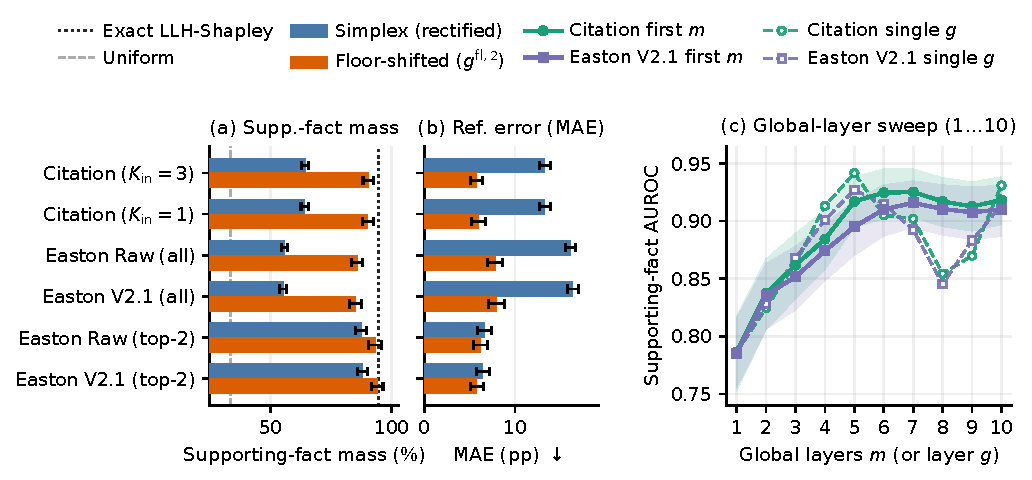
\includegraphics[width=0.98\linewidth]{figures/fig_citation_easton.pdf}
\caption{Direct attention heuristics on $200$ HotpotQA instances ($95\%$ bootstrap CIs). (a,~b)~Simplex (rectified) versus floor-shifted ($g^{\mathrm{fl},2}$) normalization on \texttt{mean10} for supporting-fact mass and MAE against exact LLH-Shapley. (c)~Supporting-fact AUROC across global-layer counts $m \in \{1, \dots, 10\}$ when averaging the first $m$ global layers (\texttt{first}~$m$, solid with $95\%$ CI bands) versus each individual global layer $\ell_g = 6g - 1$ (\texttt{single}~$g$, dashed).}
\label{fig:exp_citation_easton}
\end{figure}

\paragraph{Independent span scoring versus competitive per-step filtering.}
Both heuristics rank snippets accurately on HotpotQA (\texttt{mean10} AUROC $0.91$--$0.92$, P@2 $84.5$--$85.5\%$, Pearson $r = 0.91$--$0.92$), but they behave very differently under simplex normalization (Figure~\ref{fig:exp_citation_easton}(a,b)). Because Citation evaluates each snippet independently, entity-overlapping distractors always receive positive background attention, leaving $35.7\%$ ($42.5\%$ under \texttt{max10}) of the simplex mass on distractors and yielding $13.3$\,pp MAE. Applying $g^{\text{fl},2}$ removes this common floor without altering rankings, cutting Citation MAE from $13.3$ to $5.7$\,pp and lifting supporting-fact mass from $64.3\%$ to $90.6\%$. Conversely, Easton's competitive global \texttt{top-2} filter acts as an implicit hard floor: on $96.0\%$ of instances (\texttt{mean10}; $80.5\%$ under \texttt{max10}), at least one distractor receives exact zero weight ($\min_i s_i = 0$), so simplex normalization already achieves $6.4$\,pp MAE and $88.2\%$ supporting-fact mass ($5.8$\,pp and $94.3\%$ under $g^{\text{fl},2}$). Dropping the \texttt{top-2} filter (\emph{all tokens}) reintroduces background accumulation across distractor tokens, degrading supporting-fact mass to $55.3\%$ and AUROC to $0.88$.

\paragraph{Frequency penalty and head reduction.}
In Easton \texttt{top-2} (\texttt{mean10}), the most-attended snippet token is selected a median of $6$ times across the response; dampening repeats by $1/\sqrt{\operatorname{occ}_t(s)}$ in V2.1 consistently improves P@2 ($82.2\% \to 84.5\%$), AUROC ($0.90 \to 0.91$), Spearman $\rho$ ($0.76 \to 0.77$), and MAE ($6.6 \to 6.4$\,pp). Without per-step sparsification (\emph{all tokens}), however, every context token is included at every step so $\operatorname{occ}_t(s) = t$ merely reweights step $t$ by $t^{-1/2}$ rather than penalizing repeated token hits (whereas combining \emph{all tokens} with Stage-1 \texttt{max10+sp6} restores AUROC $0.90$ and $87.2\%$ mass). Across head reductions, averaging global heads and layers slightly outperforms elementwise maximization unless Stage-1 prefix pruning suppresses noisy outlier heads (\texttt{max10+sp24} lowers rectified Citation MAE from $15.8$ to $11.9$\,pp; \texttt{max10+sp6} raises Easton V2.1 Spearman $\rho$ to $0.78$).

\paragraph{How many global layers are worth aggregating?}
Sweeping every bottom-up prefix of $m \in \{1, \dots, 10\}$ global layers ($\ell \le 6m - 1$, matching early-exit serving budgets) reveals rapid initial gains followed by a sharp knee at half network depth (Figure~\ref{fig:exp_citation_easton}(c) and Table~\ref{tab:exp_citation_easton}). From $m = 1$ ($\ell = 5$) to $m = 5$ ($\ell \le 29$), supporting-fact AUROC climbs from $0.79$ to $0.92$ ($0.79 \to 0.84 \to 0.86 \to 0.88 \to 0.92$) for Citation and from $0.79$ to $0.90$ ($0.79 \to 0.84 \to 0.85 \to 0.87 \to 0.90$) for Easton V2.1, while MAE drops nearly in half ($11.3 \to 5.8$\,pp under $g^{\text{fl},2}$ for Citation; $12.5 \to 7.1$\,pp under simplex for Easton V2.1, as exact-zero distractor coverage rises from $58.0\%$ to $82.5\%$). By $m = 5$--$6$ ($50$--$60\%$ depth), prefix averaging already matches all $10$ global layers within $0.1$\,pp MAE, and it reaches a shallow optimum at $m = 6$--$7$ ($\ell \le 35$--$41$): at $m = 7$, Citation achieves AUROC $0.93$, P@2 $88.5\%$, $92.9\%$ mass, and $5.4$\,pp MAE, while Easton V2.1 reaches AUROC $0.92$, P@2 $86.5\%$, $89.0\%$ mass, and $6.0$\,pp MAE ($r = 0.92$, $\rho = 0.78$; elementwise maximization \texttt{max}$m$ and \texttt{max}$m$\texttt{+sp}$B$ saturate at the same $m = 6$--$7$ window). Including the remaining layers $m = 8$--$10$ brings no further improvement (P@2 softens slightly by $2$--$3$\,pp), so aggregating the first $6$--$7$ global layers---or $5$ under a tighter serving budget---captures the full accuracy while saving $30$--$50\%$ of global-layer extraction. Evaluating each global layer in isolation (\texttt{single}$g$, dashed curves in Figure~\ref{fig:exp_citation_easton}(c)) explains why: early layers $g = 1$--$3$ ($\ell \in \{5, 11, 17\}$) route a median $25.5$--$39.1\%$ of response attention to the BOS sink token (vs.\ $5.5$--$11.7\%$ in $g = 4$--$10$), single-layer accuracy peaks at the exact network midpoint $g = 5$ ($\ell = 29$; Citation AUROC $0.94$, P@2 $90.0\%$; Easton V2.1 AUROC $0.93$, P@2 $88.2\%$), dips in layers $g = 8$--$9$ ($\ell \in \{47, 53\}$, AUROC $0.85$--$0.88$), and rebounds at the final global layer $g = 10$ ($\ell = 59$, \texttt{last1}: Citation AUROC $0.93$, P@2 $88.0\%$, $5.8$\,pp MAE; Easton V2.1 AUROC $0.91$, P@2 $86.8\%$, $6.3$\,pp MAE). Contiguous bottom-up prefixes therefore require $m \ge 5$--$6$ layers to dilute early BOS-sink layers, whereas unrestricted layer selection can match or exceed $10$-layer averaging from a single mid-network or final global layer ($\ell = 29$ or $\ell = 59$).

\paragraph{Across benchmarks.}
Table~\ref{tab:exp_citation_easton_multi} evaluates the best-performing reductions on the other benchmarks with the same protocol and references as Table~\ref{tab:exp_multi}. The heuristics stay strong whenever the evidence is spread over distinct snippets: on 2WikiMultihopQA, Citation and Easton V2.1 reach AUROC $0.99$ and $r = 0.88$--$0.92$, and on CNN/DailyMail, where many sentences contribute to the summary, Easton V2.1 (\texttt{mean7}) reaches $r = 0.93$ and LDS $0.90$, more than any two-pass geometric method and close to ContextCite with $32$ ablations. On MuSiQue, Citation (\texttt{mean7}) reaches the highest supporting-fact AUROC of all methods ($0.94$, P@$k$ $80.7\%$) and Easton V2.1 $r = 0.94$, matching VATT with $v_{\text{logvol}}$. The duplicated-paragraph variant exposes limitation~(ii) below: the agreement of both heuristics with the reference drops to $r = 0.81$--$0.83$, and Easton V2.1 (\texttt{mean10}) gives one of the two copies less than $1\%$ of their joint credit in $19\%$ of the instances, because both copies compete for the same per-step top-$2$ tokens and the first match wins.

\begin{table}[t]
\centering
\small
\setlength{\tabcolsep}{3pt}
\resizebox{\linewidth}{!}{%
\begin{tabular}{llccccccccccccccc}
\toprule
 &  & \multicolumn{3}{c}{HotpotQA} & \multicolumn{3}{c}{2Wiki} & \multicolumn{3}{c}{MuSiQue} & \multicolumn{3}{c}{CNN/DM} & \multicolumn{3}{c}{Dup.} \\
\cmidrule(lr){3-5} \cmidrule(lr){6-8} \cmidrule(lr){9-11} \cmidrule(lr){12-14} \cmidrule(lr){15-17}
Heuristic & Link & $r$ & AUROC & MAE & $r$ & AUROC & MAE & $r$ & AUROC & MAE & $r$ & LDS & MAE & $r$ & AUROC & MAE \\
\midrule
Citation (\texttt{mean10}) & floor & 0.92 & 0.92 & 5.7 & 0.89 & 0.99 & 4.3 & 0.93 & 0.94 & 2.0 & 0.92 & 0.89 & 2.0 & 0.82 & 0.90 & 7.6 \\
Citation (\texttt{mean7}) & floor & 0.92 & 0.93 & 5.4 & 0.88 & 0.99 & 4.6 & 0.93 & 0.94 & 1.9 & 0.92 & 0.88 & 2.0 & 0.83 & 0.91 & 7.1 \\
Citation (\texttt{single5}) & floor & 0.89 & 0.94 & 6.2 & 0.85 & 0.99 & 5.0 & 0.90 & 0.94 & 2.5 & 0.87 & 0.85 & 2.6 & 0.83 & 0.93 & 6.6 \\
Easton V2.1 (\texttt{mean10}) & rect. & 0.92 & 0.91 & 6.4 & 0.91 & 0.99 & 3.9 & 0.94 & 0.92 & 1.8 & 0.93 & 0.89 & 1.8 & 0.81 & 0.88 & 8.2 \\
Easton V2.1 (\texttt{mean7}) & rect. & 0.92 & 0.92 & 6.0 & 0.92 & 0.99 & 3.8 & 0.94 & 0.93 & 1.8 & 0.93 & 0.89 & 1.8 & 0.82 & 0.89 & 7.9 \\
\midrule
VATT $v_{\mathrm{proj}}$ (for comparison) & floor & 0.91 & 0.93 & 5.8 & 0.88 & 0.99 & 4.6 & 0.91 & 0.90 & 2.9 & 0.85 & 0.85 & 2.9 & 0.84 & 0.91 & 6.7 \\
\bottomrule
\end{tabular}%
}
\caption{Direct attention heuristics across benchmarks (agreement with the reference of each benchmark; AUROC for supporting facts, LDS for CNN/DailyMail). VATT is repeated for comparison.}
\label{tab:exp_citation_easton_multi}
\end{table}

\paragraph{Structural limitations relative to cooperative-game attribution.}
Strong agreement on HotpotQA reflects its \emph{non-redundant} two-hop design: when two distinct paragraphs supply complementary facts, decoding attention aligns closely with ablation impact. Unlike cooperative-game values, however, raw attention heuristics lack three structural guarantees: (i)~\emph{uncalibrated context share}---context snippets absorb a median of only $43.5\%$ of \texttt{mean10} response attention (while the BOS sink token alone absorbs $15.8\%$) and unnormalized Citation totals depend strongly on the head reduction (median $\sum_i s_i^{\text{cit}} = 0.071$ on \texttt{mean10} vs.\ $1.88$ on \texttt{max10}), so separating parametric prior from context still requires the empty-context pass $w$; (ii)~\emph{no redundancy splitting}---scoring snippets independently gives two identical copies of a supporting paragraph the same raw score up to positional effects, so their combined simplex share is not split by a game but follows the attention pattern (split ratio $0.23$--$0.26$ on duplicated HotpotQA, vs.\ $0.39$ for the exact reference); and (iii)~\emph{routing versus counterfactual utility}---attention measures token lookup rather than causal entailment (e.g.\ attending to verify or negate a contradictory snippet, or favoring later positions under causal recency bias).


\end{document}